%%%%%%%%%%%%%%%%%%%%%%%%%%%%%%%%%%%%%%%%%%  不使用 authblk 包制作标题  %%%%%%%%%%%%%%%%%%%%%%%%%%%%%%%%%%%%%%%%%%%%%%
%-------------------------------PPT Title-------------------------------------
\title{第一原理计算方法与应用简介}
%-----------------------------------------------------------------------------

%----------------------------Author & Date------------------------------------
%\author[\textrm{Jun\_Jiang}]{姜\;\;骏\inst{}} %[]{} (optional, use only with lots of authors)
%% - Give the names in the same order as the appear in the paper.
%% - Use the \inst{?} command only if the authors have different
%%   affiliation.
\institute[BCC]{\inst{}%
%\institute[Gain~Strong]{\inst{}%
\vskip -20pt 北京市计算中心~云平台事业部~姜骏}
%\vskip -20pt {\large 格致斯创~科技}}
\date[\today] % (optional, should be abbreviation of conference name)
{	{\fontsize{6.2pt}{4.2pt}\selectfont{\textcolor{blue}{E-mail:~}\url{jiangjun@bcc.ac.cn}}}
\vskip 45 pt {\fontsize{8.2pt}{6.2pt}\selectfont{北京科技大学~~理化楼\textrm{-308}% 报告地点
	\vskip 5 pt \textrm{2024.07.10}}}
}

%% - Either use conference name or its abbreviation
%% - Not really information to the audience, more for people (including
%%   yourself) who are reading the slides onlin%%   yourself) who are reading the slides onlin%%   yourself) who are reading the slides onlineee
%%%%%%%%%%%%%%%%%%%%%%%%%%%%%%%%%%%%%%%%%%%%%%%%%%%%%%%%%%%%%%%%%%%%%%%%%%%%%%%%%%%%%%%%%%%%%%%%%%%%%%%%%%%%%%%%%%%%%

\subject{}
% This is only inserted into the PDF information catalog. Can be left
% out.
%\maketitle
\frame
{
%	\frametitle{\fontsize{9.5pt}{5.2pt}\selectfont{\textcolor{orange}{“高通量并发式材料计算算法与软件”年度检查}}}
\titlepage
}
%-----------------------------------------------------------------------------

%------------------------------------------------------------------------------列出全文 outline ---------------------------------------------------------------------------------
\section*{}
\frame[allowframebreaks]
{
  \frametitle{Outline}
%  \frametitle{\textcolor{mycolor}{\secname}}
  \tableofcontents%[current,currentsection,currentsubsection]
}
%%在每个section之前列出全部Outline
%%类似的在每个subsection之前列出全部Outline是\AtBeginSubsection[]
%\AtBeginSection[]
%{
%  \frame<handout:0>%[allowframebreaks]
%  {
%    \frametitle{Outline}
%%全部Outline中,本部分加亮
%    \tableofcontents[current,currentsection]
%  }
%}

%-----------------------------------------------PPT main Body------------------------------------------------------------------------------------
\small
%\section{引言}
\frame
{
	\frametitle{\textit{ab~initio}和\textrm{first~principle}}
	\begin{itemize}
		\item \textit{ab~initio}是拉丁文词汇\textrm{(Latin~term)},其含义是\textrm{``from the beginning''},由拉丁文\textit{ab}~\textrm{(``from'')}+\textit{initio}~\textrm{(``beginning'')}合成,后者是\textit{initium}的单数夺格\footnote{\fontsize{5.5pt}{4.2pt}\selectfont{夺格\textrm{(ablative)},又称离格或从格,语法功能上表示某些词汇的状语。拉丁文\textit{initium}的意思是''开始、初始''。}}
		\item \textit{ab~initio}常用于法律和科学领域,如从头计算法(\textit{ab~initio}~\textrm{method})。法律中,\textit{ab~initio}表示"一开始即如此,而非法院宣判之后"。
		\item \textrm{first~principle}指从基本的物理学定律出发,不外加假设与经验拟合的推导与计算。
		\item 在物理学领域,\textrm{first~principle}(第一性原理)和\textit{ab~initio}(从头计算)含义上是等价的。例如利用\textrm{Schr\"odinger}方程在一些近似条件下求解电子结构,但无须依赖实验数据得到拟合参数的方法,就是第一原理或从头计算法。
	\end{itemize}
}

\frame
{
	\frametitle{\textit{ab~initio} \textrm{in inscription}}
\begin{figure}[h!]
\vspace*{-0.15in}
\centering
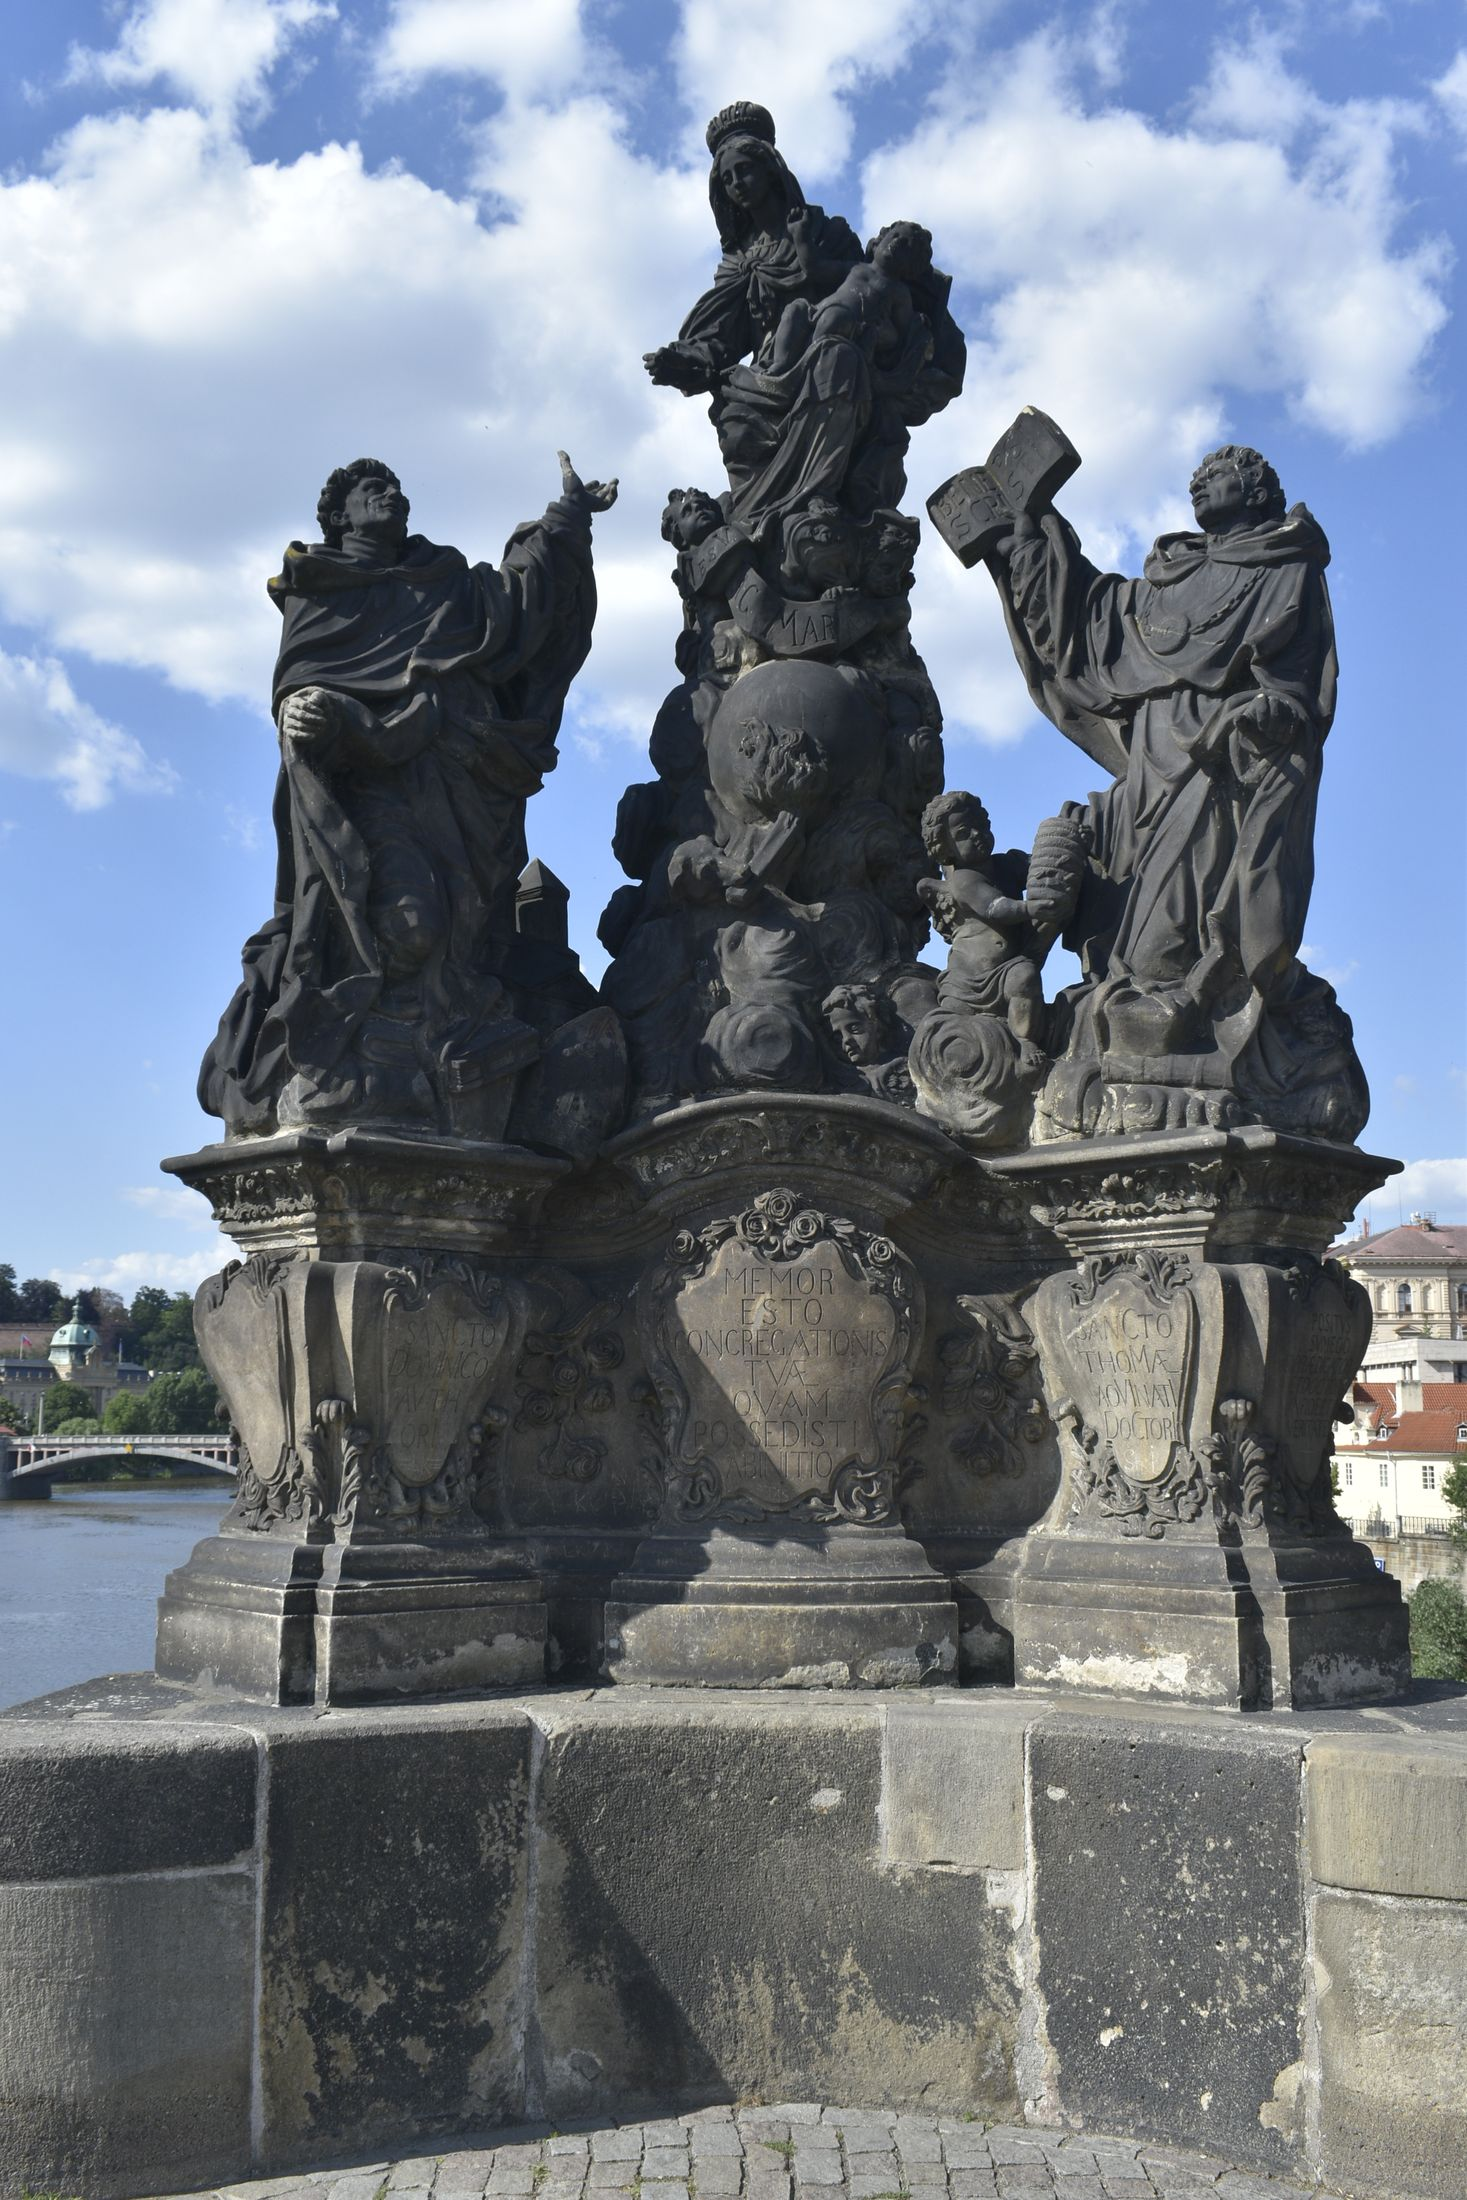
\includegraphics[height=2.10in,width=1.55in,viewport=5 3 1550 2180,clip]{Figures/Madonna-Ss.-Dominic-and-Thomas_Aquinas-3.jpeg}
\hspace*{15pt}
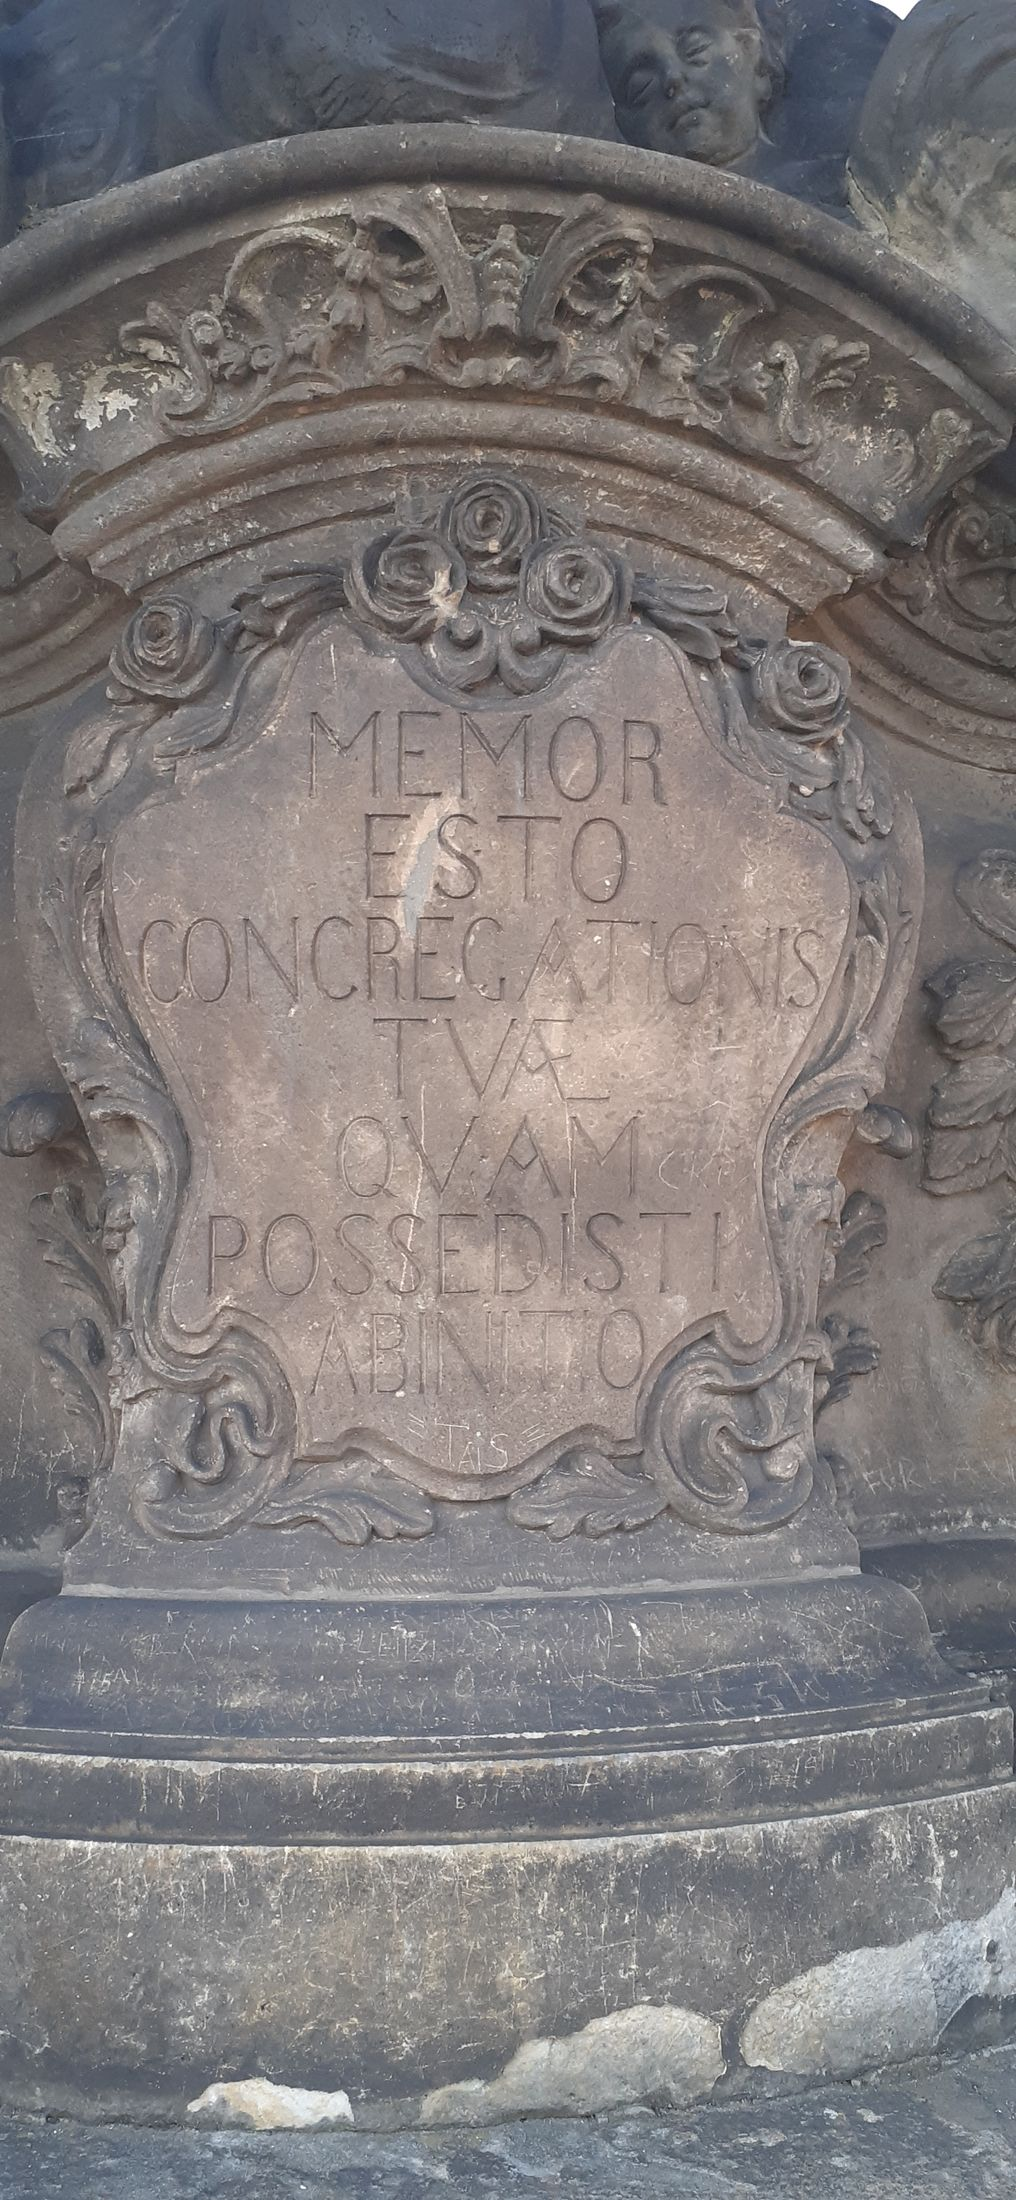
\includegraphics[height=2.10in,width=1.15in,viewport=5 3 950 1880,clip]{Figures/Madonna-Ss.-Dominic-and-Thomas_Aquinas-Inscription_2.jpeg}
%\caption{\tiny \textrm{Pseudopotential for metallic sodium, based on the empty core model and screened by the Thomas-Fermi dielectric function.}}%(与文献\cite{EPJB33-47_2003}图1对比)
\label{ABINITIO-inscription}
\end{figure}
\begin{minipage}{0.53\textwidth}
	{\fontsize{8.2pt}{4.2pt}\selectfont{ 
		\centering{MEMOR}\\
		\centering{ESTO}\\
		\centering{CONGREGATIONIS}\\
		\centering{TV\AE}\\
		\centering{QVAM}\\
		\centering{POSSEDISTI}\\
		\centering{\textcolor{red}{ABINITIO}\\}}}
\end{minipage}
\hspace*{5pt}
\begin{minipage}{0.30\textwidth}
	\textrm{\fontsize{4.2pt}{4.2pt}\selectfont{The inscription in English:}}\\
	\textrm{\fontsize{8.2pt}{4.2pt}\selectfont{\textcolor{blue}{Mind the congregation that has been yours} \textcolor{purple}{since the beginning}}}
\end{minipage}
}

%-----------------------------------------------------------------------------------------------------------------------------------------------------------------------%
\section{密度泛函理论}       %Bookmark
\subsection{\rm{Thomas-Fermi~}模型}       %Bookmark
\frame
{
	\frametitle{\textrm{Thomas-Fermi}模型} 
	1927年,\textrm{Thomas}和\textrm{Fermi}基于均匀电子气模型上建立\textrm{Thomas-Fermi}模型,\textcolor{blue}{体系能量可用}\textcolor{red}{电子密度}\textcolor{blue}{表示}:
	\begin{itemize}
		\item 动能表达式
			$$T_{\mathrm{TF}}[\rho(\vec r)]=\dfrac3{10}(3\pi^2)^{\frac23}\int\rho^{\frac53}(\vec r)\mathrm{d}\vec r$$
		\item 外势$V_{ext}(\vec r)$下电子体系的能量泛函表达式为
			\begin{displaymath}
				\begin{aligned}
					E_{\mathrm{TF}}[\rho(\vec r)]=&\dfrac3{10}(3\pi^2)^{\frac23}\int\rho^{\frac53}(\vec r)\mathrm{d}\vec r\\
					&+\int\rho(\vec r)V_{ext}(\vec r)\mathrm{d}\vec r+\dfrac12\int\int\dfrac{\rho(\vec r_1)\rho(\vec r_2)}{|\vec r_2-\vec r_1|}\mathrm{d}\vec r_1\mathrm{d}\vec r_2
				\end{aligned}
			\end{displaymath}
		\item \textrm{Thomas-Fermi}模型完全没有考虑电子的交换-相关作用
	\end{itemize}
}

\frame
{
	\frametitle{\textrm{Thomas-Fermi-Dirac}模型} 
	1930年,\textrm{Dirac}将\textrm{Thomas-Fermi}模型修正,用局域密度近似考虑电子交换作用
			\begin{displaymath}
				\begin{aligned}
					E_{\mathrm{TFD}}[\rho(\vec r)]=&\dfrac3{10}(3\pi^2)^{\frac23}\int\rho^{\frac53}(\vec r)\mathrm{d}\vec r+\int\rho(\vec r)V_{ext}(\vec r)\mathrm{d}\vec r\\
					&+\dfrac12\int\int\dfrac{\rho(\vec r_1)\rho(\vec r_2)}{|\vec r_2-\vec r_1|}\mathrm{d}\vec r_1\mathrm{d}\vec r_2-\dfrac34\bigg(\dfrac3{\pi}\bigg)^{\frac13}\int\rho^{\frac43}(\vec r)\mathrm{d}\vec r
				\end{aligned}
			\end{displaymath}
			\begin{itemize}
				\item 在总电子数守恒约束条件
					$$\int\rho(\vec r)\mathrm{d}\vec r=N$$
					下,能量泛函$E_{\mathrm{TFD}}[\rho(\vec r)]$对密度$\rho(\vec r)$的变分极小获得体系的基态密度和基态能量
			\end{itemize}
}

\frame
{
	\frametitle{\textrm{Thomas-Fermi}模型}
	\begin{itemize}
		\item \textrm{Thomas-Fermi}模型用电子密度代替波函数描述问题是极大的简化,但模型过于粗糙:\\
%			\begin{enumerate}
%				\item 以均匀电子气的密度得到动能的表达式
%				\item 完全忽略电子间的交换-相关作用
%			\end{enumerate}
			不能正确描述相互作用电子体系的基本特征,如原子的壳层结构
		\item \textrm{Thomas-Fermi}模型虽不够精确,但可以通过引入修正项校正:
			\textrm{Dirac}交换泛函 $$E_X[\rho(\vec r)]=-\dfrac34\bigg(\dfrac3{\pi}\bigg)^{\frac13}\int\rho^{\frac43}(\vec r)\mathrm{d}\vec r$$
			\textrm{Wigner}相关泛函 $$E_C[\rho(\vec r)]=-0.056\int\dfrac{\rho^{\frac43}(\vec r)}{0.079+\rho^{\frac13}(\vec r)}\mathrm{d}\vec r$$
	\end{itemize}
	\textrm{Thomas-Fermi}模型为密度泛函理论\textrm{(DFT)}提供了重要的启示
}

\frame
{
	\frametitle{电荷密度代替电子}
\begin{figure}[h!]
\centering
\vspace{3.5pt}
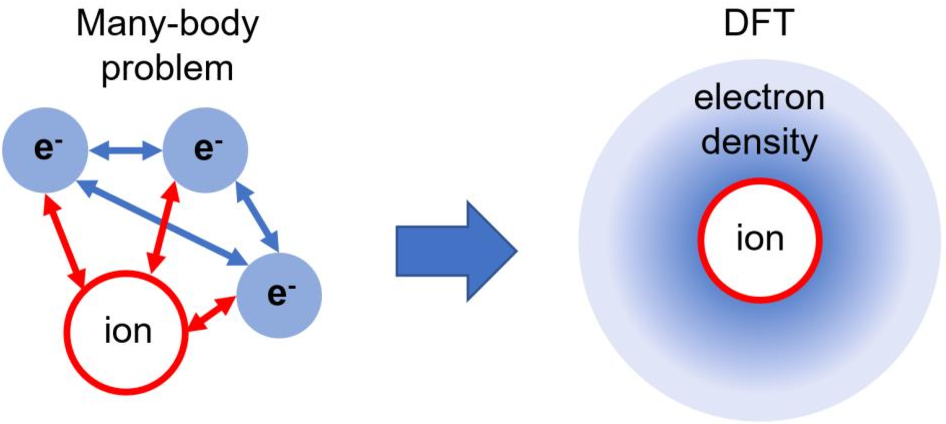
\includegraphics[height=0.45\textwidth,width=1.0\textwidth,viewport=0 0 950 440,clip]{Figures/Schematic-illustration-of-transforming-many_electron-system-to-electron-density.png}
\caption{\fontsize{6.0pt}{4.5pt}\selectfont{\textrm{Schematic illustration of transforming many-electron system to electron density.}}}
\label{Density-Particle}
\end{figure}
}

\subsection{密度泛函理论}       %Bookmark
\frame                               %
{
\frametitle{密度泛函理论(\textrm{DFT})} %Slide Page Title
%   \secname
与传统的量子力学方法不同,密度泛函理论的基本变量是体系的基态电子密度。%通过体系的电子密度而非波函数确定体系的基态能量。
\begin{itemize}%[+-| alert@+>]
	\item 密度泛函理论的基石:\textrm{Hohenberg-Kohn}定理\upcite{PR136-B864_1964}
\vskip 5pt
\begin{itemize}%[+-| alert@+>]
   \setlength{\itemsep}{8pt}
 \item $E[\rho]=F_{\mathrm{HK}}[\rho]+\displaystyle\int\rho(\vec{r})v(\vec{r})\textrm{d}\vec{r}$ \\
\vskip 5pt 其中$F_{\mathrm{HK}}[\rho]=\underset{\Psi\to\rho}{\mathrm{Min}}\langle\Psi[\rho]|\hat{T}+\hat{W}|\Psi[\rho]\rangle$
是普适的泛函表达式。%,指明多电子体系的基态性质与基态密度间存在一一对应关系
     \textrm{\small{第一定理表明多电子体系的性质完全由体系的基态密度决定}}
   \item 如果$\tilde\Psi\neq\Psi$,
     $E[\tilde\rho]\geqslant E[\rho_0]$\\
     \textrm{\small{第二定理指出基态总能量泛函在体系基态电子密度处取极小值}}
   \end{itemize}
%\textrm{\small{第二定理指出基态总能量泛函在体系基态电子密度处取极小值}}
\vskip 8pt
 \item 密度泛函理论的优越性:用密度($\rho$)代替波函数($\Psi$)描述体系
\vskip 5pt
 \item 密度泛函理论的困难:能量密度泛函的精确形式未知
   \end{itemize}
}

\frame
{
	\frametitle{\rm{Creators of DFT}}
\begin{figure}[h!]
\vskip 10pt
\centering
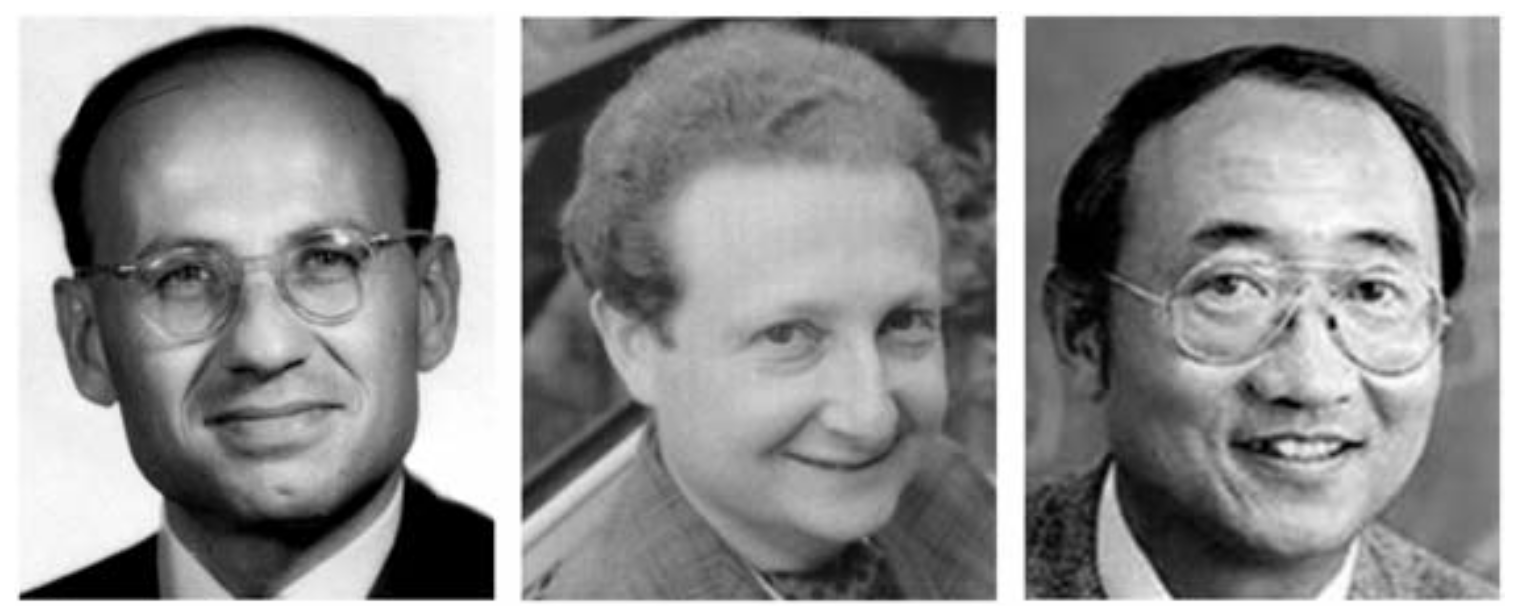
\includegraphics[height=1.65in,width=4.0in,viewport=0 0 1562 610,clip]{Figures/Creators_of_DFT.png}
\caption{\tiny \textrm{Creators of DFT. Walter Kohn(left, in 1962) and his two postdoctoral fellows, Pierre Hohenberg (middle, in 1965) and Lujeu Sham (right).}}%(与文献\cite{EPJB33-47_2003}图1对比)
\label{Creator_of_DFT}
\end{figure}
}

\frame                               %
{
\frametitle{密度泛函理论(\textrm{DFT})}
\textrm{Kohn-Sham}方程\upcite{PR140-A1133_1965}:无相互作用体系+交换-相关能的贡献
$$(T_S+V_{e\!f\!f})|\varphi_i\rangle=\varepsilon_i|\varphi_i\rangle,\quad i=1,\cdots,N,\cdots$$
其中$T_S=-\dfrac12\nabla^2$~~是无相互作用体系的动能
\begin{displaymath}
	\begin{aligned}
		V_{e\!f\!f}(\vec r)=&V_{ext}(\vec r)+\displaystyle\int w(\vec r,\vec r\,')\rho(\vec r\,')\mathrm{d}\vec r\,'+V_{\mathrm{XC}}[\rho]\\
=&\displaystyle\int\dfrac{\rho(\vec r\,')}{|\vec r-\vec r^{\prime}|}\mathrm{d}\vec r\,'+V_{ext}(\vec r)+V_{\mathrm{XC}}[\rho]
	\end{aligned}
\end{displaymath}
$V_{ext}(\vec r)$是电子体系与外部的电荷或磁场相互作用\\
$V_{\mathrm{XC}}[\rho]=\dfrac{\delta E_{\mathrm{XC}}}{\delta\rho(\vec r)}$称为交换-相关势
\vskip 10pt
\textrm{Kohn-Sham}方程是形式上的单粒子方程
\vskip 6pt
\textrm{Kohn-Sham}方程的实质:\\\textcolor{red}{将动能泛函的主要部分分离出来,剩余部分放在交换-相关能中}
}

\frame
{
	\frametitle{密度\textrm{vs.}粒子与泛函表示}
\begin{figure}[h!]
\vskip -10pt
\centering
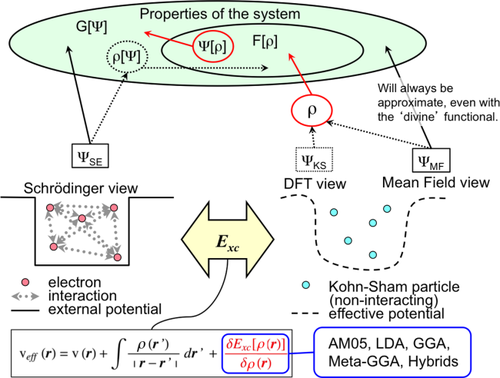
\includegraphics[height=2.65in,width=3.8in,viewport=0 0 362 275,clip]{Figures/DFT-particle-density.png}
\caption{\fontsize{6.0pt}{4.5pt}\selectfont{\textrm{Properties of a quantum mechanical system can be calculated by solving the SE (left). A more tractable, formally equivalent way is to solve the DFT KS equations (right).}}}%(与文献\cite{EPJB33-47_2003}图1对比)
\label{Schrodinger-equation-vs-Kohn-Sham-equation}
\end{figure}
}

\frame
{
	\frametitle{}
\begin{figure}[h!]
\centering
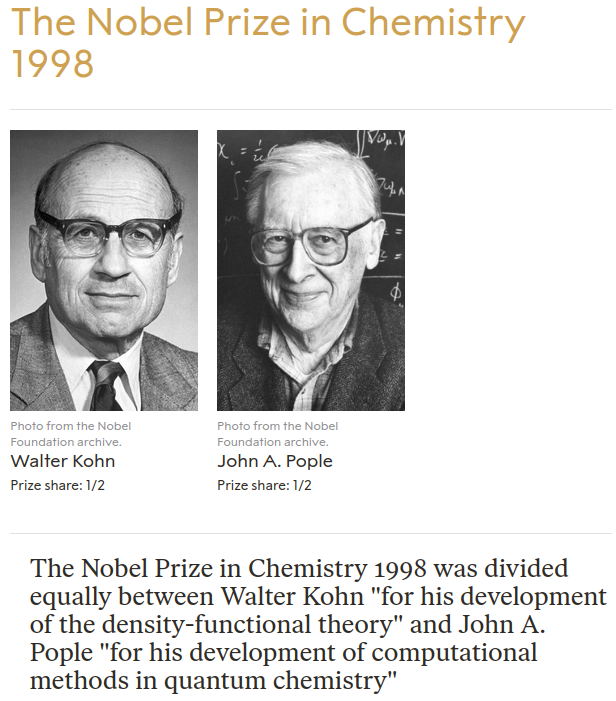
\includegraphics[height=2.65in,width=3.0in,viewport=0 0 600 570,clip]{Figures/Nobel_Prize_Chemistry_1998.png}
\caption{\tiny \textrm{The Nolbel Prize in Chemistry 1998 Summary.}}%(与文献\cite{EPJB33-47_2003}图1对比)
\label{Nobel_Prize_for_Chemistry}
\end{figure}
}

\frame
{
\frametitle{交换-相关能与交换-相关势}
实际考虑交换-相关能时,会将交换-相关能表示为交换能和相关能之和:
\begin{displaymath}
	E_{\mathrm{XC}}[\rho]=E_{\mathrm{X}}[\rho]+E_{\mathrm{C}}[\rho]=\int\varepsilon_{\mathrm{X}}[\rho]\rho(\vec{r}) \textrm{d}^3\vec{r}+\int\varepsilon_{\mathrm{C}}[\rho]\rho(\vec{r}) \textrm{d}^3\vec{r}
\end{displaymath}
$\varepsilon_{\mathrm{X}}[\rho]$和$\varepsilon_{\mathrm{C}}[\rho]$可理解为单电子的交换能和相关能
\vskip 20pt
交换-相关势通过交换-相关能计算得到:~
		\begin{displaymath}
			V_{\mathrm{XC}}^{\sigma}[\rho_{\alpha},\rho_{\beta}]=\dfrac{\delta E_{\mathrm{XC}}[\rho_{\alpha},\rho_{\beta}]}{\delta\rho_{\sigma}}=\dfrac{\delta\{E_{\mathrm{X}}[\rho_{\alpha},\rho_{\beta}]+E_{\mathrm{C}}[\rho_{\alpha},\rho_{\beta}]\}}{\delta\rho_{\sigma}}
		\end{displaymath}
		\textcolor{red}{注意}:~由于$E_{\mathrm{XC}}[\rho_{\sigma}]$对$\rho_{\sigma}$是非线性的\\
		\textcolor{blue}{$V_{\mathrm{XC}}=V_{\mathrm{X}}+V_{\mathrm{C}}$和$\varepsilon_{\mathrm{XC}}=\varepsilon_{\mathrm{X}}+\varepsilon_{\mathrm{C}}$不同,不要混淆这两个量}
}
%  \beamertemplateshadingbackground{blue!10}{yellow!10}

\frame                               %
{
\frametitle{交换-相关能密度泛函}
\textcolor{blue}{密度泛函理论的核心问题}:\\
\textrm{Kohn-Sham}方程用于实际计算,必须知道$E_{XC}[\rho]$或者$V_{XC}[\rho]$与$\rho(\vec r)$的泛函关系
\vskip 15pt
\begin{minipage}[b]{0.59\textwidth}
 \hspace*{-15pt}
 {\fontsize{7.5pt}{6.0pt}\selectfont\begin{itemize}%[+-| alert@+>]
	 \setlength{\itemsep}{10pt}
 \item \textrm{LDA}:泛函只与密度分布的局域值有关
 \item \textrm{GGA}:泛函依赖:局域密度及其梯度
 \item $meta$-\textrm{GGA}:泛函依赖的变量还有动能密度
 \item 杂化(\textrm{hybrid})泛函:泛函与占据轨道有关
 \item 其他的交换-相关能泛函
 \item<1-> 完全非局域泛函:理想泛函,不现实
 \end{itemize}}
\end{minipage}
\hfill
\begin{minipage}[b]{0.39\textwidth}
\hspace*{-10pt}
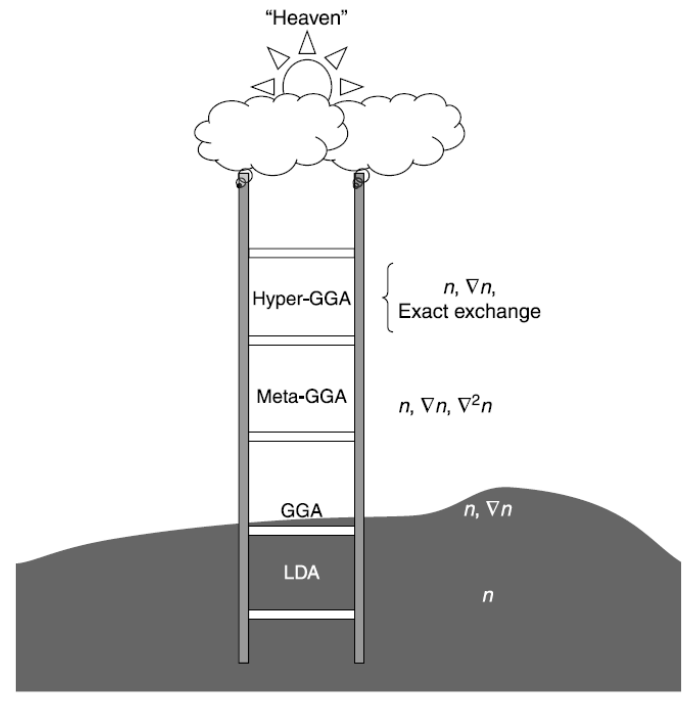
\includegraphics[height=1.7in,width=3.18in,viewport=10 5 1380 700,clip]{Figures/Jacobi-ladder.png}\\
\centering{\textcolor{red}{\textrm{\tiny Jacob's ladder}}}
\end{minipage}
% \begin{itemize}%[+-| alert@+>]
%\item 交换-相关能密度泛函
}

\frame
{
	\frametitle{探索泛函形式}
\begin{figure}[h!]
%\vskip 0.2in
\centering
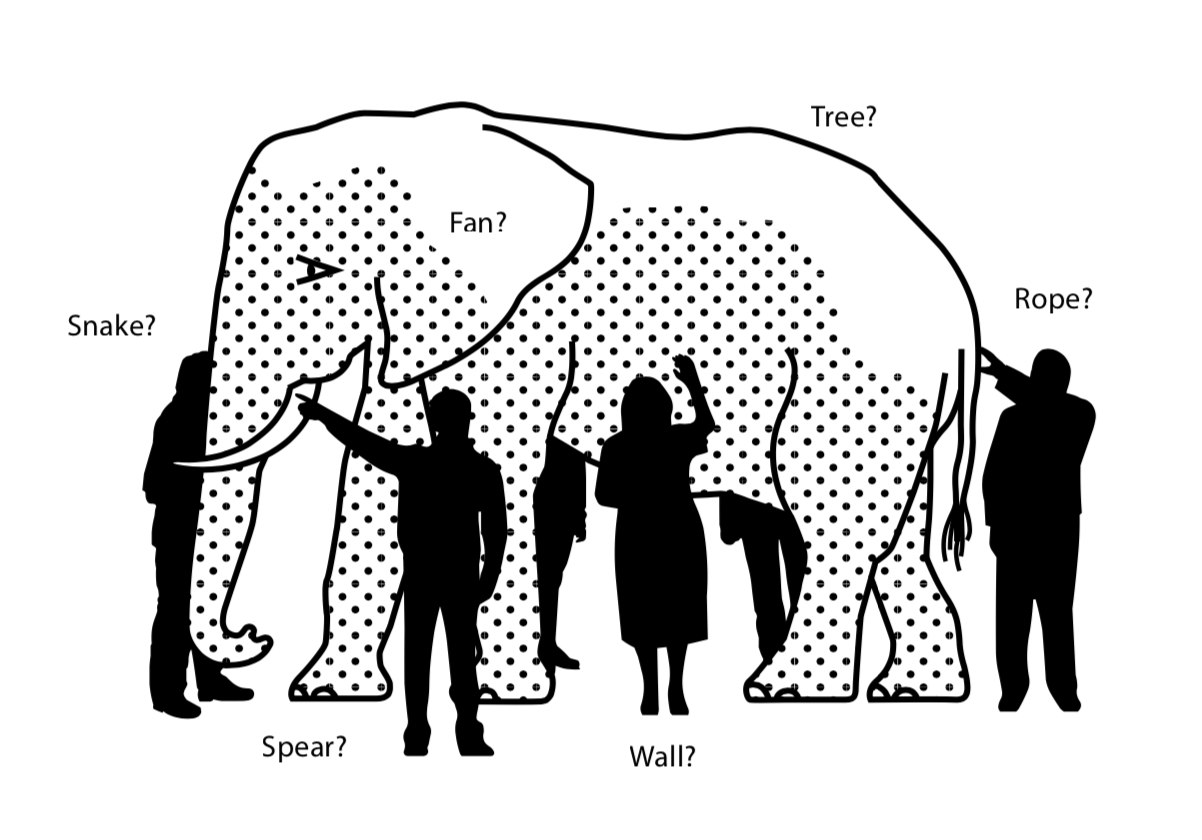
\includegraphics[height=2.3in,width=4.0in,viewport=0 0 601 400,clip]{Figures/Blind_men-and-Elephant.png}
%\caption{\tiny \textrm{Creators of DFT. Walter Kohn(left, in 1962) and his two postdoctoral fellows, Pierre Hohenberg (middle, in 1965) and Lujeu Sham (right).}}%(与文献\cite{EPJB33-47_2003}图1对比)
\label{Blind_man-and-elephant}
\end{figure}
}

\frame                               %
{
	\frametitle{近似能量泛函$E_{\mathrm{XC}}[\rho]$的主要问题}
\vskip 20pt
\begin{enumerate}%[+-| alert@+>]
   \setlength{\itemsep}{10pt}
 \item  密度是整体变量:~电子自相互作用抵消不净\\%\quad\textrm{(LDA+U)}方法的校正%(\textrm{LDA+U})
	 用\textrm{DFT}计算电子数很少的体系,一般都会有较大的误差
 \item  电子相关:~简并和近简并基态的表示不合理\\
	 基态电子密度用不同的简并轨道计算时,体系能量应保持不变,但现有的近似能量泛函不具有这个性质
 \item  渐近行为:~处理弱相互作用体系的误差大\\
	 如\textrm{Van der Waals}相互作用和现有近似能量泛函本身的计算误差在同一量级
 \end{enumerate}
}

\frame                               %
{
	\frametitle{\textrm{Kohn-Sham}方程}
\begin{figure}[h!]
\centering
\vspace*{-0.21in}
\hspace*{-0.1in}
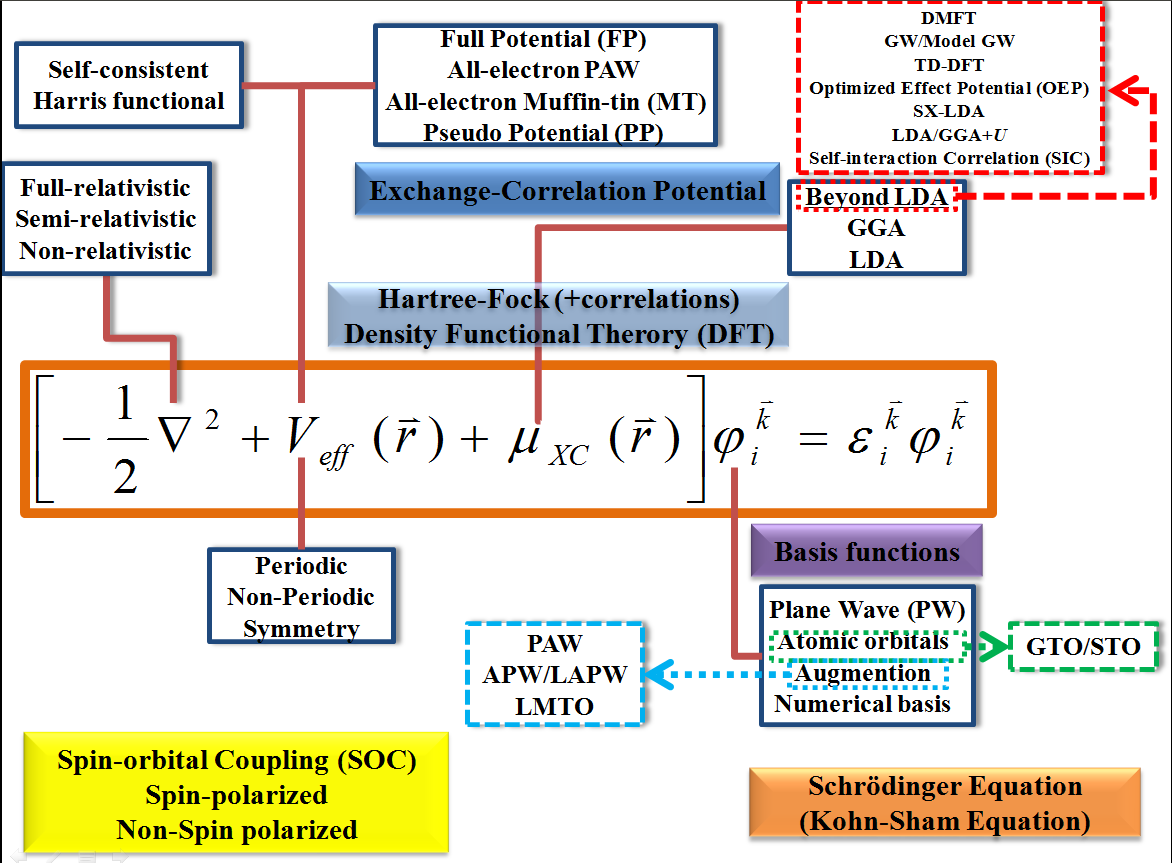
\includegraphics[height=2.7in,width=4.0in,viewport=2 5 1162 880,clip]{Figures/DFT.png}
\caption{\tiny \textrm{The Analysis of Kohn-Sham equation.}}%(与文献\cite{EPJB33-47_2003}图1对比)
\label{DFT}
\end{figure}
}

\frame
{
	\frametitle{基组:~张开空间,展开波函数}
\begin{figure}[h!]
	\vspace{-5pt}
\centering
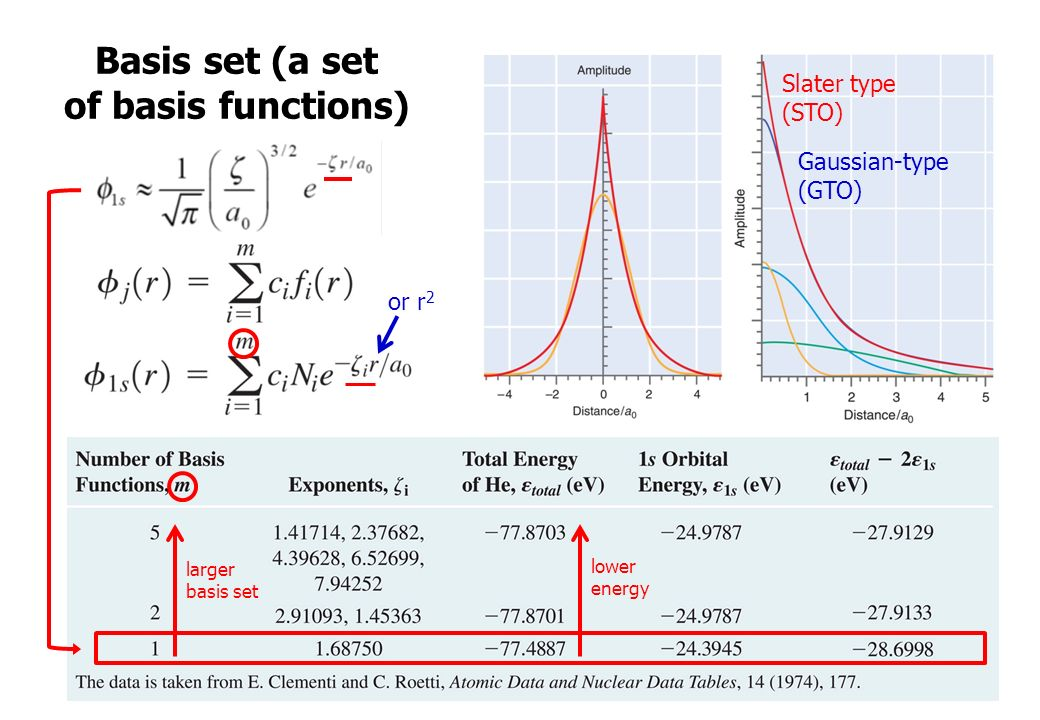
\includegraphics[height=2.6in,width=4.01in,viewport=0 0 780 550,clip]{Figures/Basis-set-STO-GTO.jpg}
\caption{\fontsize{5.5pt}{4.2pt}\selectfont{\textrm{Schematic illustration of scattering of a Basic-set STO GTO.}}}%(与文献\cite{EPJB33-47_2003}图1对比)
\label{Basic-set:STO-GTO}
\end{figure}
}

\subsection{常见泛函的一些形式}
\frame%[allowframebreaks]
{
	\frametitle{\rm{LDA}泛函}
	\begin{itemize}
		\item 交换能部分
	\begin{displaymath}
		\begin{aligned}
			\varepsilon_{\mathrm{X}}[\rho,\zeta]=&2^{-1/3}C_{\mathrm{X}}^{\sigma}g(\zeta)\rho^{1/3}(\vec r)\\
			E_{\mathrm{X}}[\rho,\zeta]=&\int\varepsilon_{\mathrm{X}}[\rho,\zeta]\rho(\vec r)\mathrm{d}\vec r\\
		\end{aligned}
	\end{displaymath}
	{\fontsize{7.5pt}{6.0pt}\selectfont{这里:~$C_{\mathrm{X}}^{\sigma}=\dfrac32\bigg(\dfrac3{4\pi}\bigg)^{1/3}$\\
		$g(\zeta)=\dfrac12\bigg[(1+\zeta)^{4/3}+(1-\zeta)^{4/3}\bigg]$\\
		$\zeta(\vec r)=\dfrac{[\rho_{\alpha}(\vec r)-\rho_{\beta}(\vec r)]}{[\rho_{\alpha}(\vec r)+\rho_{\beta}(\vec r)]}$}}
	\end{itemize}
}

\frame%[allowframebreaks]
{
	\frametitle{\rm{LDA}泛函}
	\begin{itemize}
		\item 相关能部分
			\begin{displaymath}
				\hspace*{-30pt}	\varepsilon_{\mathrm{C}}^{\mathrm{LDA}}(r_s,\zeta)=\varepsilon_{\mathrm{C}}(r_s,0)+a_{\mathrm{c}}(r_s)\dfrac{f(\zeta)}{f^{\prime\prime}(\zeta)}(1-\zeta^4)+[\varepsilon_{\mathrm{c}}(r_s,1)-\varepsilon_{\mathrm{c}}(r_s,0)]f(\zeta)\zeta^4
			\end{displaymath}
			{\fontsize{7.5pt}{6.0pt}\selectfont{这里:~$r_s=\bigg[\dfrac3{4\pi}(\rho_{\alpha}+\rho_{\beta})^{-1}\bigg]^{1/3}$~$f(\zeta)=[(1+\zeta)^{4/3}+(1-\zeta)^{4/3}-2]/(2^{4/3}-2)$\\
			$\varepsilon_{\mathrm{C}(r_s,0)}$、$\varepsilon_{\mathrm{C}(r_s,1)}$、$a_{\mathrm{C}(r_s)}$由经验公式
			\begin{displaymath}
				\begin{aligned}
					&G(r_s,A,\alpha_1,\beta_1,\beta_2+\beta_3+\beta_4)\\
					=&-2A(1+\alpha_1r_s)\ln\bigg[1+\dfrac1{2A(\beta_1r_s^{1/2}+\beta_2r_s+\beta_2r_s^{3/2}+\beta_1r_s^2)}\bigg]
				\end{aligned}
			\end{displaymath}
		计算。其中$A$、$\alpha_1$、$\beta_1$、$\beta_2$、$\beta_3$、$\beta_4$是参数,通过拟合实验结果确定}}
		\begin{displaymath}
			E_{\mathrm{C}}[\rho]=\int\rho(\vec r)\varepsilon_{\mathrm{C}}(\vec r)\mathrm{d}\vec r
		\end{displaymath}
	\end{itemize}
}

\frame%[allowframebreaks]
{
	\frametitle{\rm{GGA}泛函}
	\begin{itemize}
		\item 交换能泛函:
			\begin{itemize}
				\item \textrm{PW91}
					\begin{displaymath}
						\begin{aligned}
							E_{\mathrm{X}}^{\mathrm{PW91}}[\rho_{\alpha},\rho_{\beta}]=&\dfrac12(E_{\mathrm{X}}^{\mathrm{PW91}}[2\rho_{\alpha}]+E_{\mathrm{X}}^{\mathrm{PW91}}[2\rho_{\beta}])\\
							E_{\mathrm{X}}^{\mathrm{PW91}}[\rho]=&-\dfrac34\bigg(\dfrac3\pi\bigg)^{1/3}\int\rho^{4/3}(\vec r)F(x)\mathrm{d}\vec r
						\end{aligned}
					\end{displaymath}
					\hspace*{-30 pt}{\fontsize{4.5pt}{4.0pt}\selectfont{这里:~$F(x)=\dfrac{1+0.19645(hx)\sinh^{-1}(7.7956hx)+(hx)^2\{0.2743-0.1508\mathrm{exp}[-100(hx)^2]\}}{1+0.19645(hx)\sinh^{-1}(7.7956hx)+0.004(hx)^4}$}\\
					$h=(24\pi^2)^{-1/3}$,~~~$x=|\nabla\rho|\rho^{-4/3}$}
				\item \textrm{PBE}
			\begin{displaymath}
				E_{\mathrm{X}}^{\mathrm{PBE}}[\rho,x]=E_{\mathrm{X}}^{\mathrm{LDA}}[\rho,x]-C_{\mathrm{X}}\int a\bigg(1-\dfrac1{bx^2}\bigg)\rho^{4/3}(\vec r)\mathrm{d}\vec r
			\end{displaymath}
			{\fontsize{4.5pt}{4.0pt}\selectfont{其中:~$C_{\mathrm{X}}=\dfrac34\bigg(\dfrac3\pi\bigg)^{1/3}$\\$a=0.804$,~~~$b=0.273$~是非经验参数}}
			\end{itemize}
	\end{itemize}
}

\frame%[allowframebreaks]
{
	\frametitle{\rm{GGA}泛函}
	\begin{itemize}
		\item 相关能泛函:
			\begin{itemize}
				\item \textrm{PW91}
					\begin{displaymath}
						\begin{aligned}
							E_{\mathrm{C}}^{\mathrm{PW91}}[\rho_{\alpha},\rho_{\beta}]=&\int\mathrm{d}\vec r\rho(\vec r)[\varepsilon_{\mathrm{C}}^{\mathrm{LSDA}}(r_s,\zeta)]+H(t,r_s,\zeta)\\
							H=&H_0+H_1
						\end{aligned}
					\end{displaymath}
					{\fontsize{4.5pt}{4.0pt}\selectfont{这里:~
						\begin{displaymath}
							\begin{aligned}
								H_0=&f^3(\zeta)\dfrac{\beta^2}{2\alpha}\ln\bigg(1+\dfrac{2\alpha}{\beta}\dfrac{t^2+At^4}{1+At^2+A^2t^4}\bigg)\\
								A=&\dfrac{2\alpha}{\beta}\dfrac1{\mathrm{exp[-2\alpha\varepsilon_{\mathrm{C}}^{\mathrm{LDA}}(r_s,\zeta)}/f^3(\zeta)\beta^2]-1}\\
							t=&\dfrac{|\nabla\rho|}{2f(\zeta)k_s\rho}~~~f(\zeta)=\dfrac12\bigg[(1+\zeta)^{2/3}+(1-\zeta)^{2/3}\bigg]\\
							k_s=&[4(3\pi^{-1}\rho)^{1/3}]^{1/2}
							\end{aligned}
						\end{displaymath}
						参数 $\alpha=0.09$,~~~$\beta=\nu C_{\mathrm{C}}(0)$\\
						$\nu=(16/\pi)(3\pi^2)^{1/3}$,~~~$C_{\mathrm{C}}(0)=0.004235$
				}}
			\end{itemize}
	\end{itemize}
}

\frame%[allowframebreaks]
{
	\frametitle{\rm{meta-GGA}泛函}
	\begin{itemize}
		\item 交换能泛函
			\begin{itemize}
				\item \textrm{TPSS}
					\begin{displaymath}
						\begin{aligned}
							E_{\mathrm{X}}^{\mathrm{TPSS}}[\rho]&=\int\mathrm{d}\vec r\rho(\vec r)\varepsilon_{\mathrm{X}}^{\mathrm{LSDA}}(\vec r)F_{\mathrm{X}}^{\mathrm{TPSS}}(p,z)\\
							F_{\mathrm{X}}^{\mathrm{TPSS}}&=1+\kappa-\dfrac{\kappa}{1+x/\kappa}
						\end{aligned}
					\end{displaymath}
{\fontsize{4.5pt}{4.0pt}\selectfont{这里:~
	$\rho(\vec r)=\rho_{\alpha}(\vec r)+\rho_{\beta}({\vec r})$,~~~$\varepsilon_{\mathrm{X}}^{\mathrm{LSDA}}(\vec r)=-\dfrac3{4\pi}[3\pi^2\rho(\vec r)]^{1/3}$
\\
\begin{displaymath}
	\begin{aligned}
		x=&\left\{\bigg[\dfrac{10}{81}+\dfrac{cz^2}{(1+z^2)^2}\bigg]p+\dfrac{146}{2025}\bar{q}_b^2-\dfrac{73}{405}\bar{q}_b\bigg[\dfrac12\bigg(\dfrac35z\bigg)^2+\dfrac12p^2\bigg]^{1/2}\right.\\
		&+\left.\dfrac1{\kappa}\bigg(\dfrac{10}{81}\bigg)^2p^2\dfrac{20e^{1/2}}{81}\bigg(\dfrac35z\bigg)^2+e\mu p^3\right\}(1+e^{1/2}p)^{-2}\\
		p=&\dfrac{|\nabla\rho(\vec r)|^2}{4(3\pi^2)^{2/3}\rho^{8/3}(\vec r)}, ~~~ \bar{q}_b=\dfrac{(9/20)(\alpha-1)}{[1+b\alpha(\alpha-1)]^{1/2}}+2p/3
	\end{aligned}
\end{displaymath}
$z=\tau_w/\tau$,~~~$\tau_w=\dfrac{|\nabla\rho(\vec r)|^2}{8\rho(\vec r)}$,~~~$\tau=\sum\limits_{\sigma}\tau_{\sigma}$\\
$\alpha=(\tau-\tau_w)/\tau_{\mathrm{unif}}=(5p/3)(z^{-1}-1)$,~~~$\tau_{\mathrm{tiff}}=\dfrac3{10}(3\pi^2)^{2/3}[\rho(\vec r)]^{5/3}$
}}
			\end{itemize}
	\end{itemize}
}


\frame%[allowframebreaks]
{
	\frametitle{\rm{meta-GGA}泛函}
	\begin{itemize}
		\item 相关能泛函
			\begin{itemize}
				\item {\textrm{TPSS}}
					\begin{displaymath}
						E_{\mathrm{C}}^{\mathrm{TPSS}}[\rho_{\alpha,\rho_{\beta}}]=\int\mathrm{d}\vec r\rho(\vec r)\varepsilon_{\mathrm{C}}^{\mathrm{TPSS0}}[1+\mathrm{d}\varepsilon_{\mathrm{C}}^{\mathrm{TPSS0}}(\tau_w/\tau)^3]
					\end{displaymath}
{\fontsize{4.5pt}{4.0pt}\selectfont{这里:~
	\begin{displaymath}
		\begin{aligned}
			\varepsilon_{\mathrm{C}}^{\mathrm{TPSS0}}=&\varepsilon_{\mathrm{C}}^{\mathrm{PBE}}(\rho_{\alpha},\rho_{\beta},\nabla\rho_{\alpha},\nabla\rho_{\beta})[1+C(\zeta,\xi)(\tau_w/\tau)^2]\\
			&-\bigg[1+C(\zeta,\xi)(\tau_w/\tau)^2\sum\limits_{\sigma}\dfrac{\rho_{\sigma}(\vec r)}{\rho(\vec r)}\bar{\varepsilon}_{\mathrm{C}}\bigg]\\
			\bar{\varepsilon}_{\mathrm{C}}=&\max[\varepsilon_{\mathrm{C}}^{\mathrm{PBE}}(\rho_{\alpha},0,\nabla\rho_{\alpha},0),\varepsilon_{\mathrm{C}}^{\mathrm{PBE}}(\rho_{\alpha},\rho_{\beta},\nabla\rho_{\alpha},\nabla\rho_{\beta})]\\
			C(\zeta,\xi)=&\dfrac{C(\zeta,0)}{\{1+\xi^2[(1+\zeta)^{-4/3}+(1-\zeta)^{-4/3}]/2\}^4}
		\end{aligned}
	\end{displaymath}
	$\xi=\dfrac{|\nabla\zeta|}{2[3\pi^2\rho(\vec r)]^{1/3}}$, ~~~$C(\zeta,0)=0.53+0.87\zeta^2+0.50\zeta^4+2.26\zeta^6$
}}
			\end{itemize}
	\end{itemize}
	\vskip 5pt
	\textrm{TPSS}泛函的特点:~\\
	\vskip 3pt
	{\fontsize{7.5pt}{6.0pt}\selectfont{不包含依靠实验数据的可调参数,数字系数由精确能量泛函满足的条件确定\\
		\textcolor{blue}{对电子分布较为均匀的晶体体系和电子分布激烈变化的分子体系都有较高的精度} }}
}

\frame
{
	\frametitle{\rm{hybrid}泛函}
	体系\textrm{Hamilton}算符表示为
	\begin{displaymath}
		\hat{H}_{\lambda}=-\dfrac12\sum_i^N\nabla^2+\sum_i^NV_i(\rho,\lambda)+\dfrac{\lambda}2\sum_i^N\sum_{j(j\neq i)}^N\dfrac1{r_{ij}}
	\end{displaymath}
	\begin{displaymath}
		\mbox{\textcolor{blue}{$\lambda$表征电子间相互作用程度}}\left\{
		\begin{aligned}
			&\lambda=0:~\mbox{无相互作用的参考体系}\\
			&\lambda=1:~\mbox{存在相互作用的真实体系}
		\end{aligned}
		\right.
	\end{displaymath}
	交换-相关能表示为
	\begin{displaymath}
		\begin{aligned}
			E_{\mathrm{XC}}^{\lambda}=&\dfrac12\int\mathrm{d}\vec r_1\rho_1^{\lambda}(\vec r_1)\int\dfrac{h_{\mathrm{XC}}^{\lambda}(\vec r_1,\vec r_2)}{\vec r_1-\vec r_2}\mathrm{d}\vec r_2\\
			E_{\mathrm{XC}}=&\int E_{\mathrm{XC}}^{\lambda}\mathrm{d}\lambda
		\end{aligned}
	\end{displaymath}
	{\fontsize{4.5pt}{4.0pt}\selectfont{这里:~$h_{\mathrm{XC}}(\vec r_1,\vec r_2)=\dfrac{2\rho_2(\vec r_1,\vec r_2)}{\rho(\vec r_1)}-\rho_1(\vec r_2)$}}
}

\frame
{
	\frametitle{\rm{hybrid}泛函}
	\begin{itemize}
		\item \textrm{half-to-half}
			\begin{displaymath}
				\begin{aligned}
					E_{\mathrm{XC}}=&\dfrac12(E_{\mathrm{XC}}^0+E_{\mathrm{XC}}^1)=\dfrac12E_{\mathrm{XC}}^{\mathrm{Exact}}+\dfrac12E_{\mathrm{XC}}^1\\
					\approx&\dfrac12E_{\mathrm{XC}}^{\mathrm{HF}}+\dfrac12E_{\mathrm{XC}}^{\mathrm{LSDA}}
				\end{aligned}
			\end{displaymath}
		\item \textrm{B3LYP}
			\begin{displaymath}
			\hspace*{-20pt}	E_{\mathrm{XC}}^{\mathrm{B3LYP}}=(1-a)E_{\mathrm{X}}^{\mathrm{LSDA}}+aE_{\mathrm{X}}^{\mathrm{HF}}+b\Delta E_{\mathrm{X}}^{\mathrm{VB88}}+cE_{\mathrm{C}}^{\mathrm{LYP}}+(1-c)E_{\mathrm{C}}^{\mathrm{LSDA}}
			\end{displaymath}
	\end{itemize}
	\vskip 8pt
	\textcolor{blue}{电子间的交换能和相关能都是离域的,但长程作用方向相反,很大程度上彼此抵消,剩余部分主要是局域的,所以将交换能和相关能合在一起处理,用局域近似可以比较好地描述电子行为}\\
	\vskip 5pt
	\textcolor{red}{采用精确交换能形式,虽然消除了自相互作用的误差,但剩余的相关能主体是离域的,因此局域形式的泛函不再是好的近似,对电子行为的描述效果会变差}
}

\frame
{
	\frametitle{\rm{DFT}之歌}
\begin{figure}[h!]
	\vspace{-10pt}
\centering
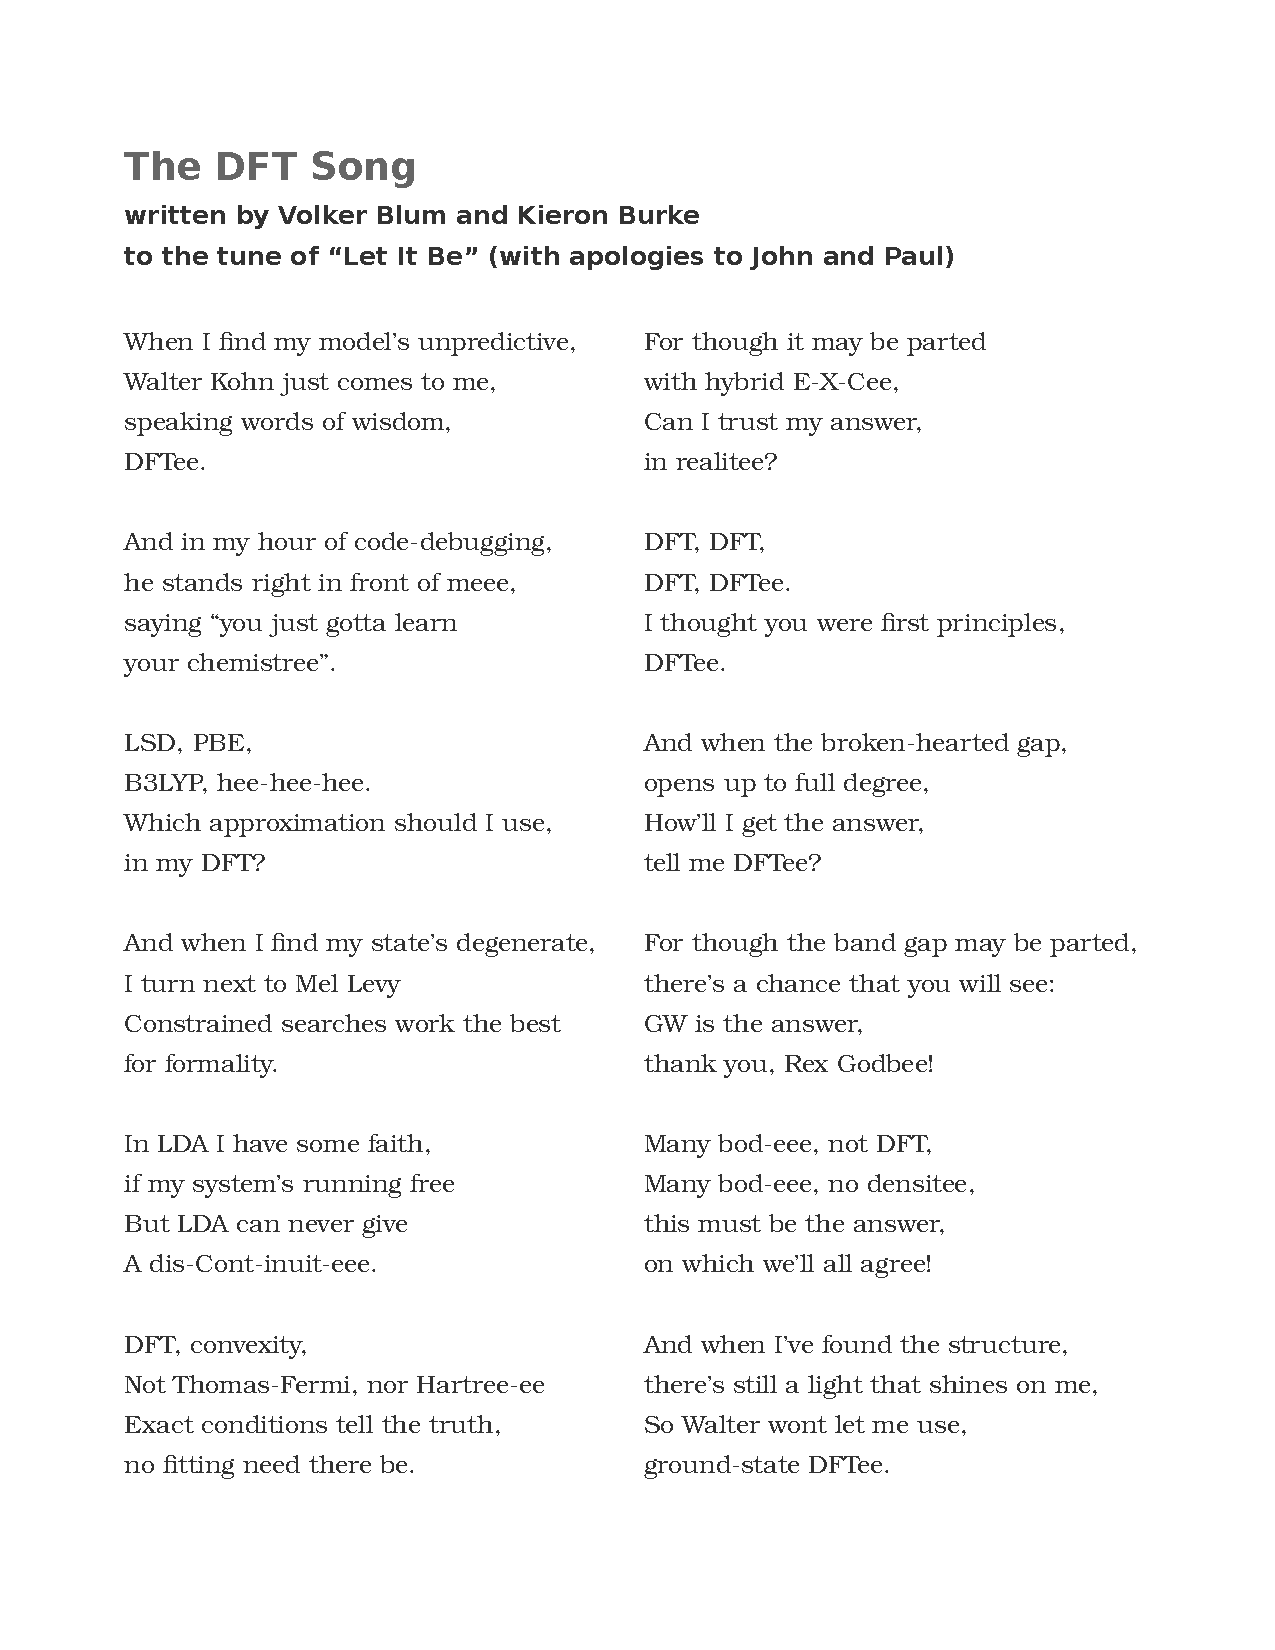
\includegraphics[height=2.85in,width=3.8in,viewport=0 350 550 720,clip]{Figures/DFT_song-1.pdf}
%\caption{\tiny \textrm{The Nolbel Prize in Chemistry 1998 Summary.}}%(与文献\cite{EPJB33-47_2003}图1对比)
\label{DFT_Song_01}
\end{figure}
}

\frame
{
	\frametitle{}
\begin{figure}[h!]
	\vspace{-10pt}
\centering
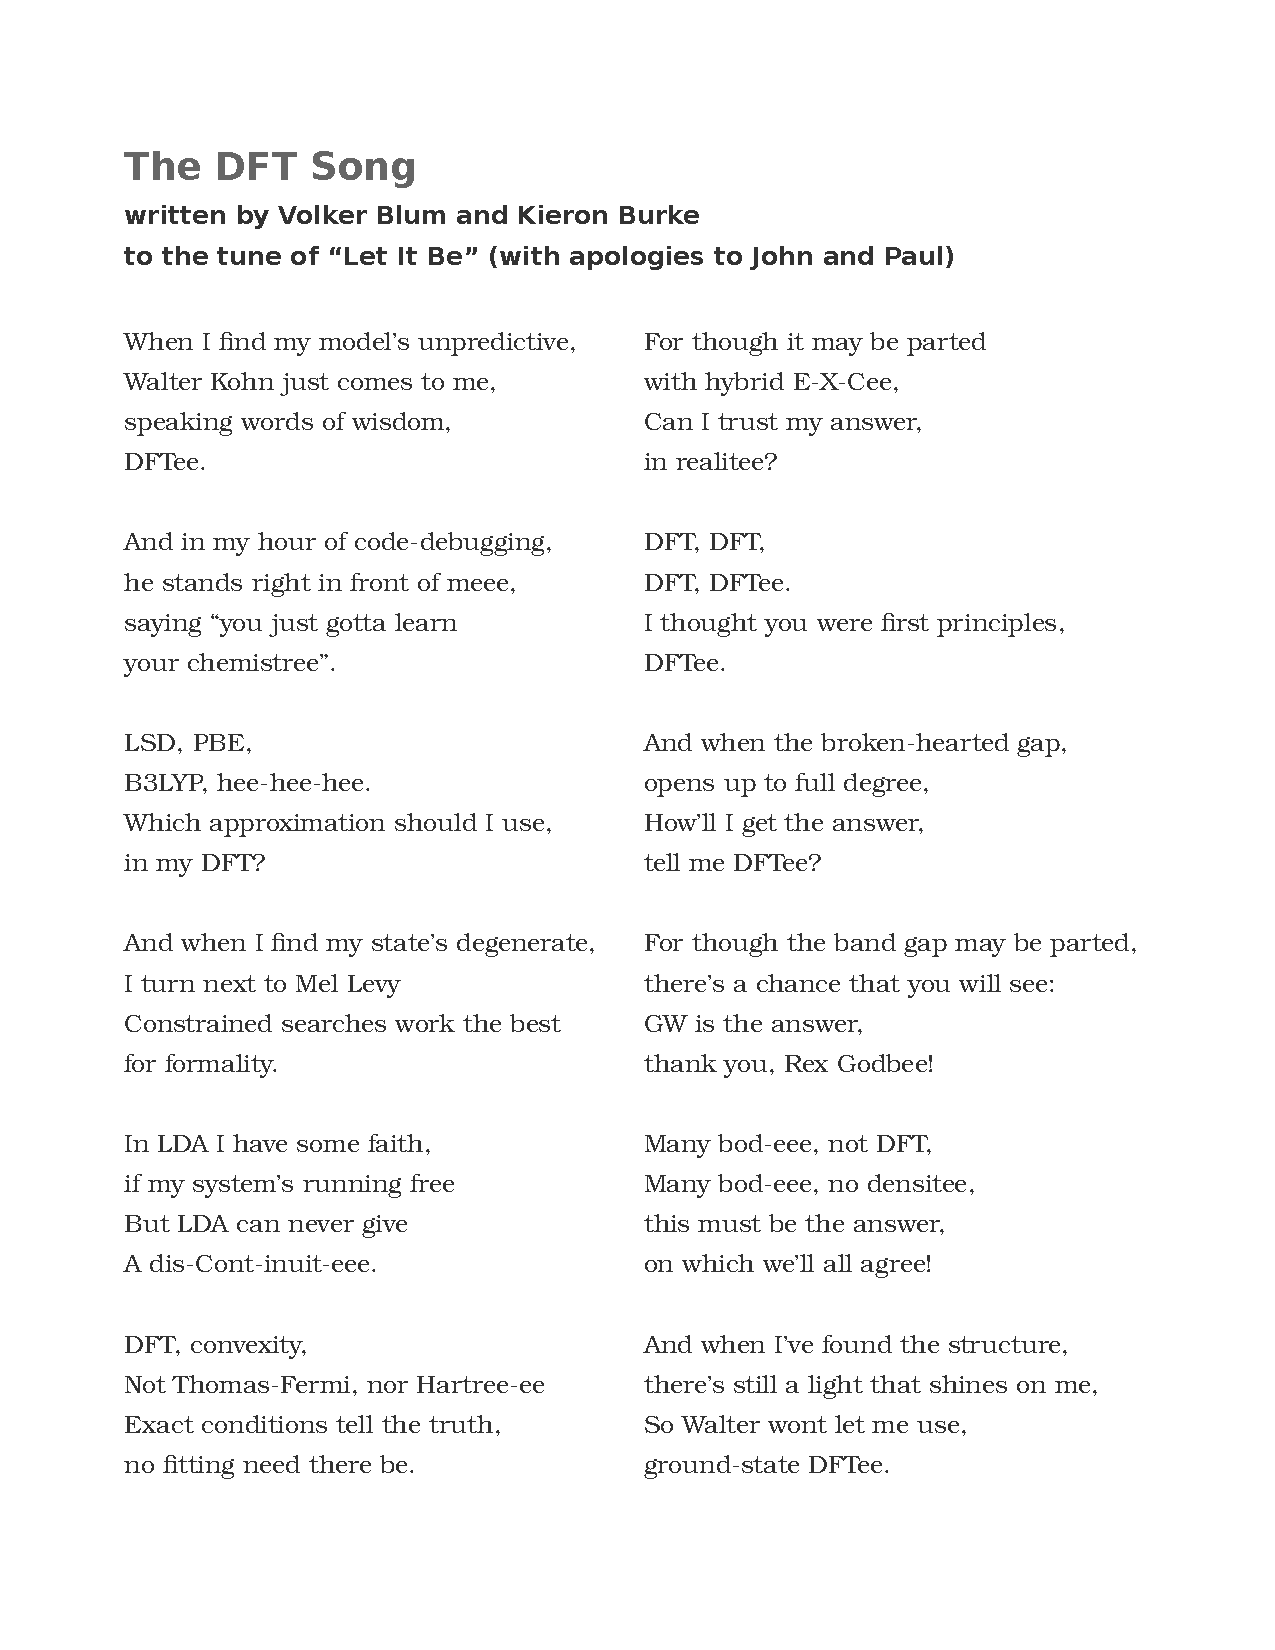
\includegraphics[height=1.95in,width=3.8in,viewport=0 80 550 352,clip]{Figures/DFT_song-1.pdf}
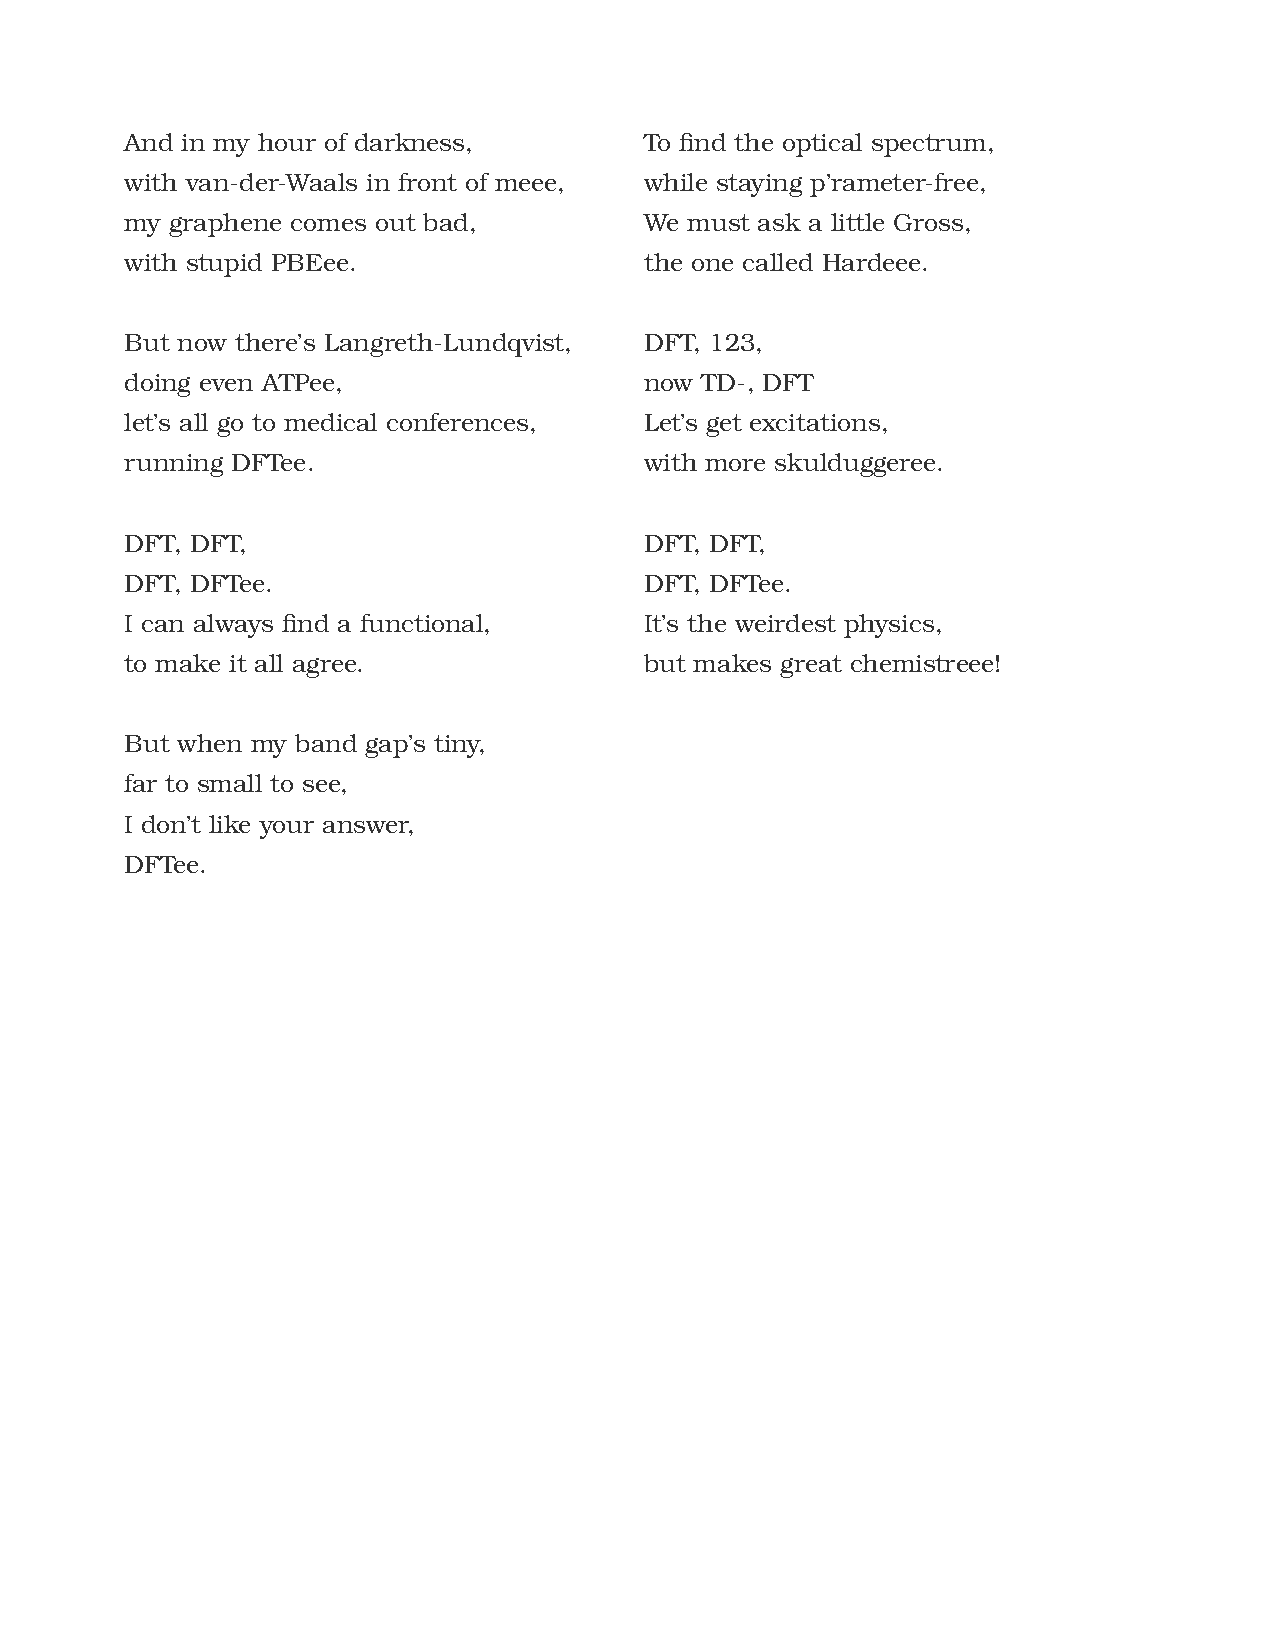
\includegraphics[height=0.70in,width=3.8in,viewport=0 650 550 750,clip]{Figures/DFT_song-2.pdf}
%\caption{\tiny \textrm{The Nolbel Prize in Chemistry 1998 Summary.}}%(与文献\cite{EPJB33-47_2003}图1对比)
\label{DFT_Song_02}
\end{figure}
}

\frame
{
	\frametitle{}
\begin{figure}[h!]
	\vspace{-10pt}
\centering
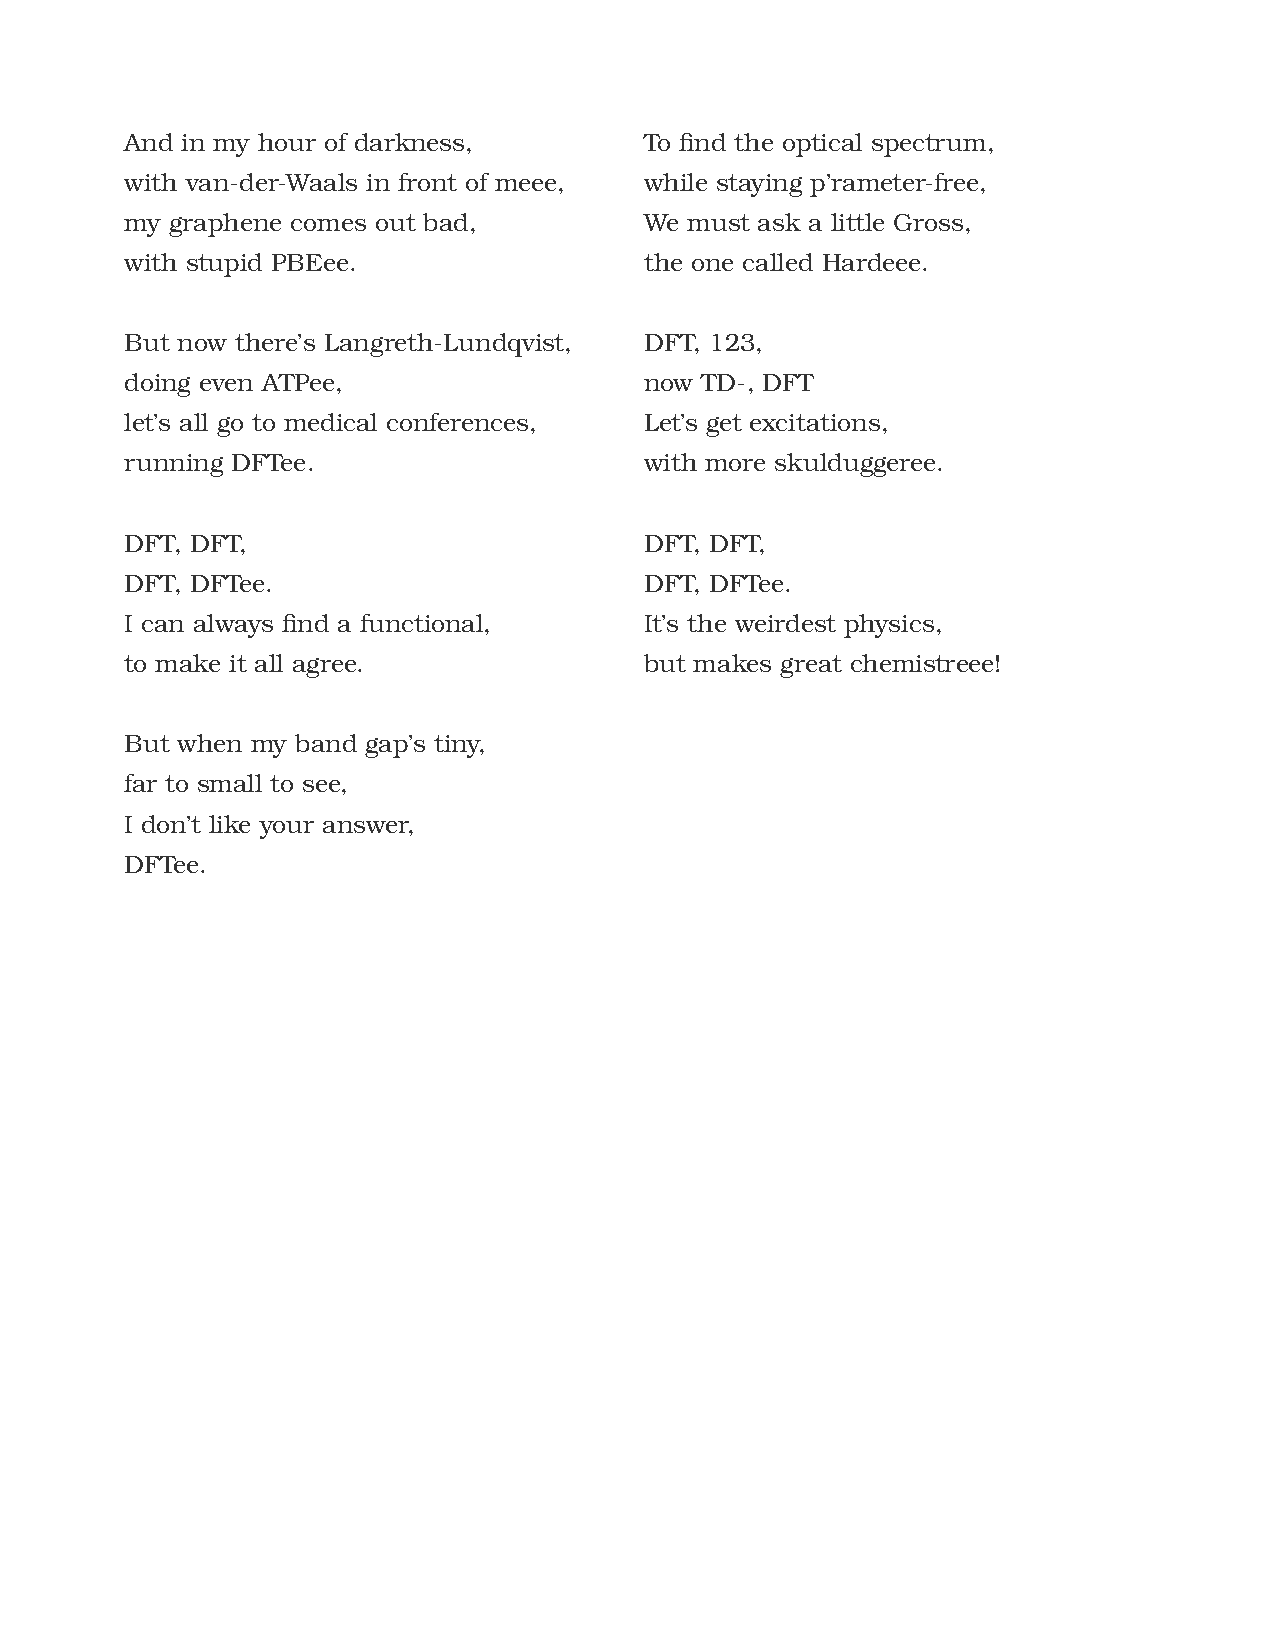
\includegraphics[height=2.10in,width=3.8in,viewport=0 350 550 650,clip]{Figures/DFT_song-2.pdf}
%\caption{\tiny \textrm{The Nolbel Prize in Chemistry 1998 Summary.}}%(与文献\cite{EPJB33-47_2003}图1对比)
\includemovie[poster, controls, mouse, url] {0.8\textwidth}{0.1\textwidth}{Figures/DFT_Song.mp3}     %
%\includemovie[poster, controls, mouse, url] {0.8\textwidth}{0.2\textwidth}{Figures/DFT_Song_accompany.mp3}     %
\label{DFT_Song_03}
\end{figure}
}
\frame
{
	\frametitle{\textrm{DFT-SCF}}
\begin{figure}[h!]
\centering
\vspace*{-0.25in}
\hspace*{-0.80in}
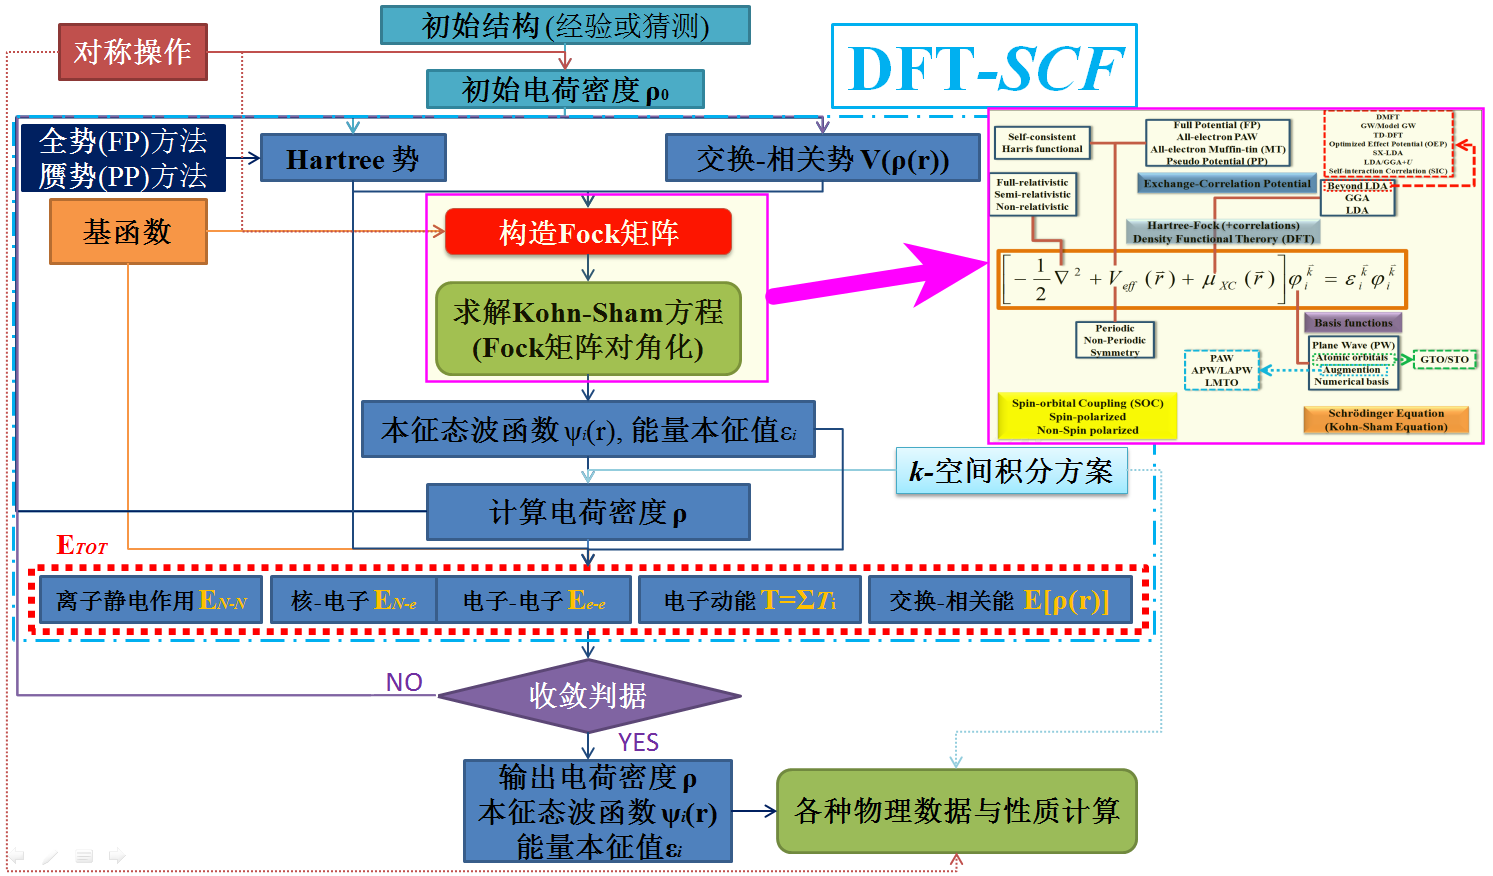
\includegraphics[height=2.80in,width=4.95in,viewport=5 3 1490 870,clip]{Figures/DFT-SCF_2.png}
%\caption{\tiny \textrm{Pseudopotential for metallic sodium, based on the empty core model and screened by the Thomas-Fermi dielectric function.}}%(与文献\cite{EPJB33-47_2003}图1对比)
\label{DFT-SCF-2}
\end{figure}
}

%------------------------------------------------------------------------Reference----------------------------------------------------------------------------------------------
\begin{thebibliography}{99}
\frame[allowframebreaks]
{
\frametitle{主要参考文献}
{\tiny
\bibitem{Xu_Li_Wang}徐光宪、黎乐民、王德民, {\textit{量子化学——基本原理和从头计算法}}\;\textrm{({\textit{上、中}})}\:科学出版社, 北京, 1980
\bibitem{PR136-B864_1964}\textrm{P. Hohenberg and W. Kohn, \textit{Phys. Rev.} \textbf{136} (1964), B864}
\bibitem{PR140-A1133_1965}\textrm{W. Kohn and L.J. Sham, \textit{Phys. Rev.} \textbf{140} (1965), A1133}
\bibitem{PRL49-1691_1982}\textrm{P. Perdew, R. G. Parr, M. Levy and J. L. Balduz, Jr., \textit{Phys. Rev. Lett.} \textbf{49} (1982), 1691}
\bibitem{Parr_Yang}\textrm{R.G. Parr and W. Yang. \textit{Density-Functional Theory of Atoms and Molecules} (Oxford University Press, New York, U.S.A., 1989)}
}
\nocite*{}
}
\end{thebibliography}

%-----------------------------------------------------------------------------
\section{固体能带理论}       %Bookmark
\frame
{
%\frametitle{The Bloch theorem}
	\frametitle{\textrm{Bloch~}定理}
\begin{itemize}%[+-| alert@+>]
   \setlength{\itemsep}{8pt}
   \item 固体能带理论\upcite{Huang-Han}是固体电子理论的基础,形式上是单电子理论:
    $$\hat H |\psi_i^{\vec k}(\vec r)\rangle=\bigg[-\dfrac{\hbar^2}{2m}\nabla^2+V(\vec r)\bigg]|\psi_i^{\vec k}(\vec r)\rangle=\epsilon_i(\vec k)|\psi_i^{\vec k}(\vec r)\rangle$$
  \item \textrm{Bloch}定理:
%   \item \textrm{periodic potential:} $$V(\vec r)=V(\vec r+\vec R_n)$$
%     \textrm{Here,} $\vec R_n=n\vec R$
%   \item \textrm{Bloch theorem:}$$\psi_{\vec k}(\vec r)=\textrm{e}^{\textrm i\vec k\cdot\vec r}u_{\vec k}(\vec r)$$
%     \textrm{Here, $u_{\vec k}(\vec r)$ is a periodic function with the same periodicity as $V(\vec r)$, i.e., $u_{\vec k}(\vec r)=u_{\vec k}(\vec r+\vec R_n)$, then Bloch theorem could reads as:}
%     $$\psi_{\vec k}(\vec r+\vec R_n)=\textrm{e}^{\textrm i\vec k\cdot\vec R_n}\psi_{\vec k}(\vec r)$$
具有平移周期性的理想晶体,势能$V(\vec r)$满足$$V(\vec r)=V(\vec r+\vec R_n)$$
体系的波函数满足\textrm{Bloch}波函数形式:$$\psi_{\vec k}(\vec r)=\textrm{e}^{i\vec k\cdot\vec r}u_{\vec k}(\vec r)$$
是平面波和周期函数的乘积。$u(\vec r)$与势能有相同的周期。即$$u_{\vec k}(\vec r)=u_{\vec k}(\vec r+\vec R_n)$$
  \item 能带理论相当于分子轨道理论
%   \setlength{\itemsep}{30pt}
\item \textrm{Bloch}函数反映了波函数在周期性势场下的变化规律。
\end{itemize}
}

\frame
{
\frametitle{周期体系的波函数}
物质的电子体系,可分为芯层分子和价层电子。芯电子能量低,受周围化学环境影响很小,基本保持原子属性;价层电子相互作用较强,对化学环境较为敏感。一般地,价电子波函数在原子间区域(\textrm{Interstitial}区)的变化平缓,在临近原子核附近区域(\textrm{Muffin-tin}球内),会出现剧烈振荡(与芯层波函数正交)。
\begin{figure}[h!]
\centering
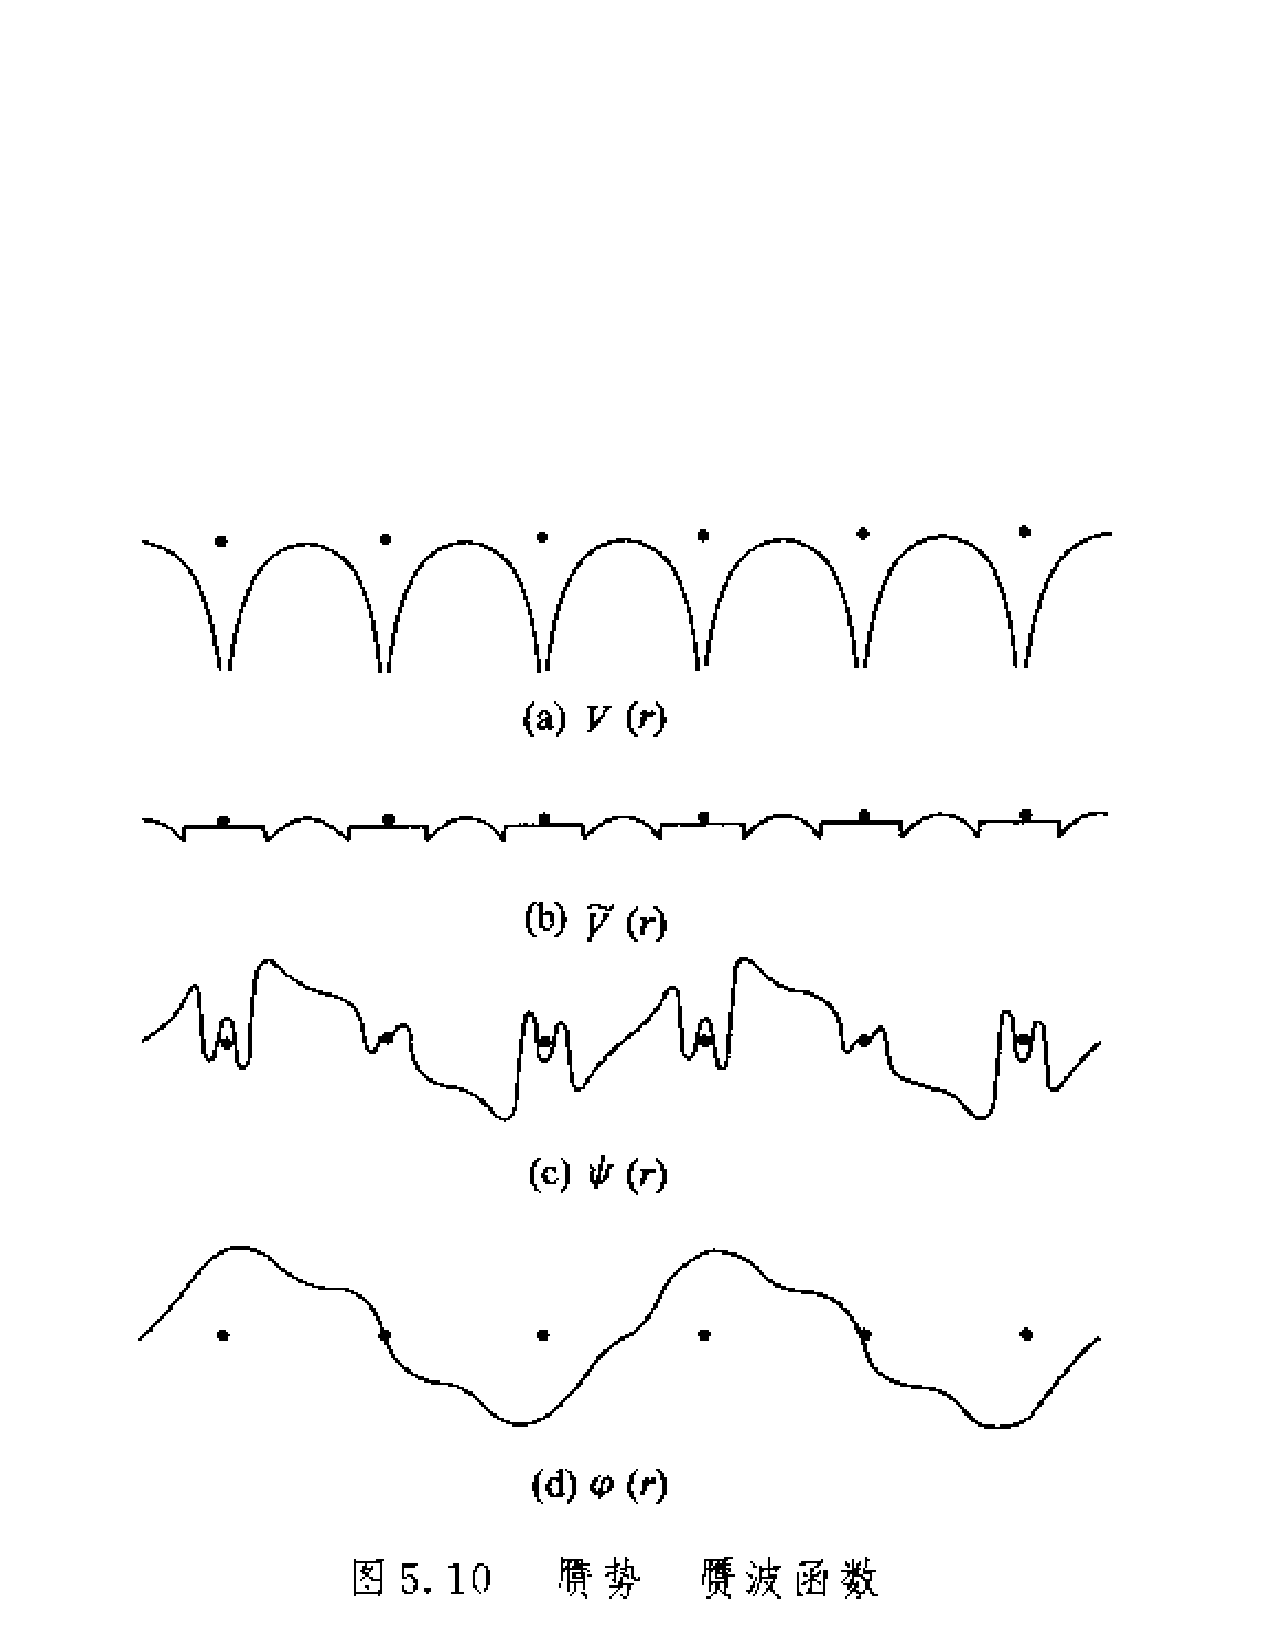
\includegraphics[height=0.8in,width=4.in,viewport=41 433 539 546,clip]{Figures/Pseudo_wave.pdf}\\
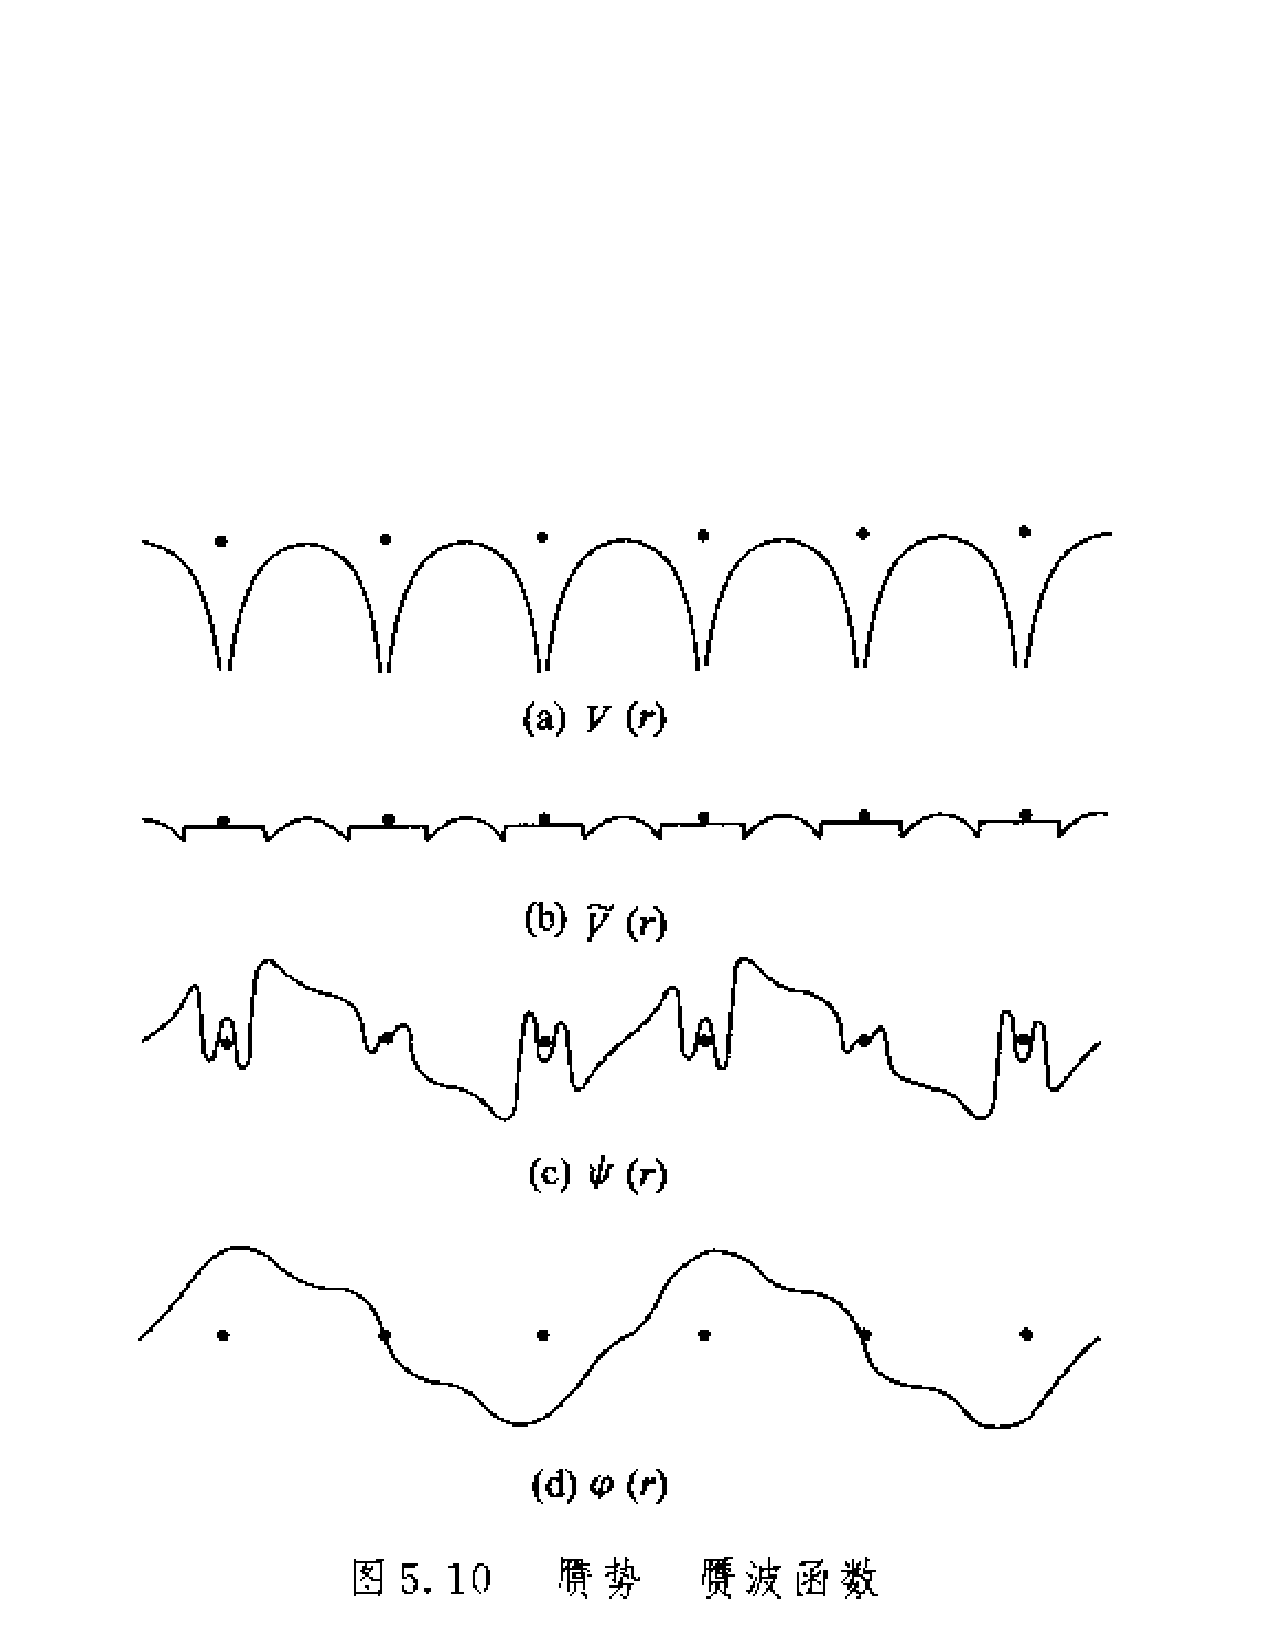
\includegraphics[height=0.8in,width=4.in,viewport=41 210 539 339,clip]{Figures/Pseudo_wave.pdf}
\caption{\tiny \textrm{The periodic Potential and the wave functions in crystal.}}%(与文献\cite{EPJB33-47_2003}图1对比)
\label{Potential-Wave}
\end{figure}
}

\frame
{
\frametitle{一维自由电子近似微扰}
\begin{figure}[h!]
\centering
%\hspace*{-10pt}
%\vspace*{-1.1in}
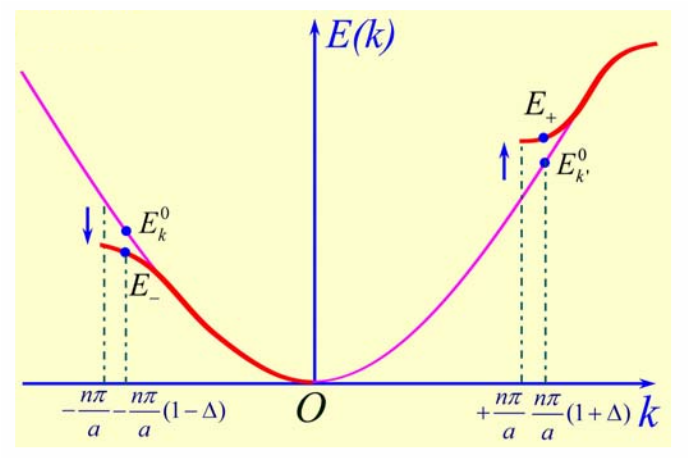
\includegraphics[height=1.5in,width=2.5in,viewport=5 5 700 450,clip]{Figures/Band_Gap-2.png}
%\caption{\tiny \textrm{The Band-structure from free-electron gas.}}%
\label{Band-Gap-2}
\end{figure} 
\begin{displaymath}
	\begin{aligned}
		&\hat H_0=-\dfrac{\hbar^2}{2m}\dfrac{\mathrm{d}^2}{\mathrm{d}x^2}+\={V} \longrightarrow \hat H=\hat H_0+\hat H^{\prime}=-\dfrac{\hbar^2}{2m}\dfrac{\mathrm{d}^2}{\mathrm{d}x^2}+\={V}+\underline{V(x)-\={V}}\\
		&\Psi_k^0(x)=\dfrac1{\sqrt V}\mathrm{e}^{\mathrm{i}k\cdot x} \longrightarrow \Psi_k(x)=\Psi_k^0(x)+\sum_{k^{\prime}\neq k}\dfrac{\langle k^{\prime}|\hat H^{\prime}|k\rangle}{E_k^0-E_{k^{\prime}}^0}\Psi_{k^{\prime}}^0(x)\\
		&\hat E_k^0=-\dfrac{\hbar^2k^2}{2m}+\={V} \longrightarrow E_k=%E_k^0+E^{\prime}=
		\dfrac{\hbar^2k^2}{2m}+\={V}+\sum_n{}^{\prime}\dfrac{|V_n|^2}{\frac{\hbar^2}{2m}[k^2-(k+2\pi\frac na)^2]}
	\end{aligned}
\end{displaymath}
}

\frame
{
\frametitle{一维自由电子简并微扰}
在波矢$k=\pm\frac{n\pi}{a}$位置,电子能量出现简并态,必须采用简并态微扰理论处理
\begin{figure}[h!]
\centering
%\hspace*{-10pt}
%\vspace*{-1.1in}
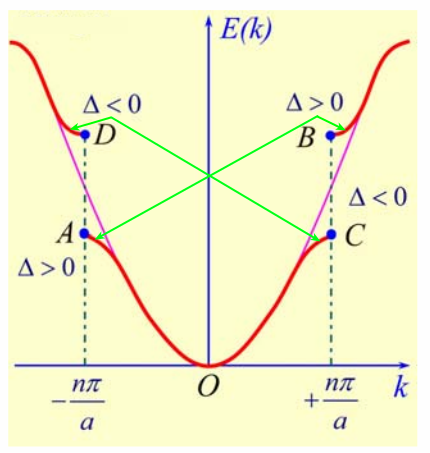
\includegraphics[height=1.3in,width=1.4in,viewport=0 5 420 450,clip]{Figures/Band_Gap-1.png}
%\caption{\tiny \textrm{The Band-structure from free-electron gas.}}%
\label{Band-Gap-1}
\end{figure} 
\begin{displaymath}
	E_{\textcolor{red}{\pm}}=\left\{
	\begin{aligned}
		&T_n+\={V}\textcolor{red}{+}\Delta^2T_n\bigg(\dfrac{2T_n}{|V_n|}\textcolor{red}{+}1\bigg)\\
		&T_n+\={V}\textcolor{red}{-}\Delta^2T_n\bigg(\dfrac{2T_n}{|V_n|}\textcolor{red}{-}1\bigg)
	\end{aligned}\right.
\end{displaymath}
这里$T_n=\frac{\hbar^2}{2m}\big(\frac{n\pi}a\big)^2$
}

\frame
{
\frametitle{自由电子气模型}
简并态微扰理论引起的能带裂分
\begin{figure}[h!]
\centering
%\hspace*{-10pt}
%\vspace*{-1.1in}
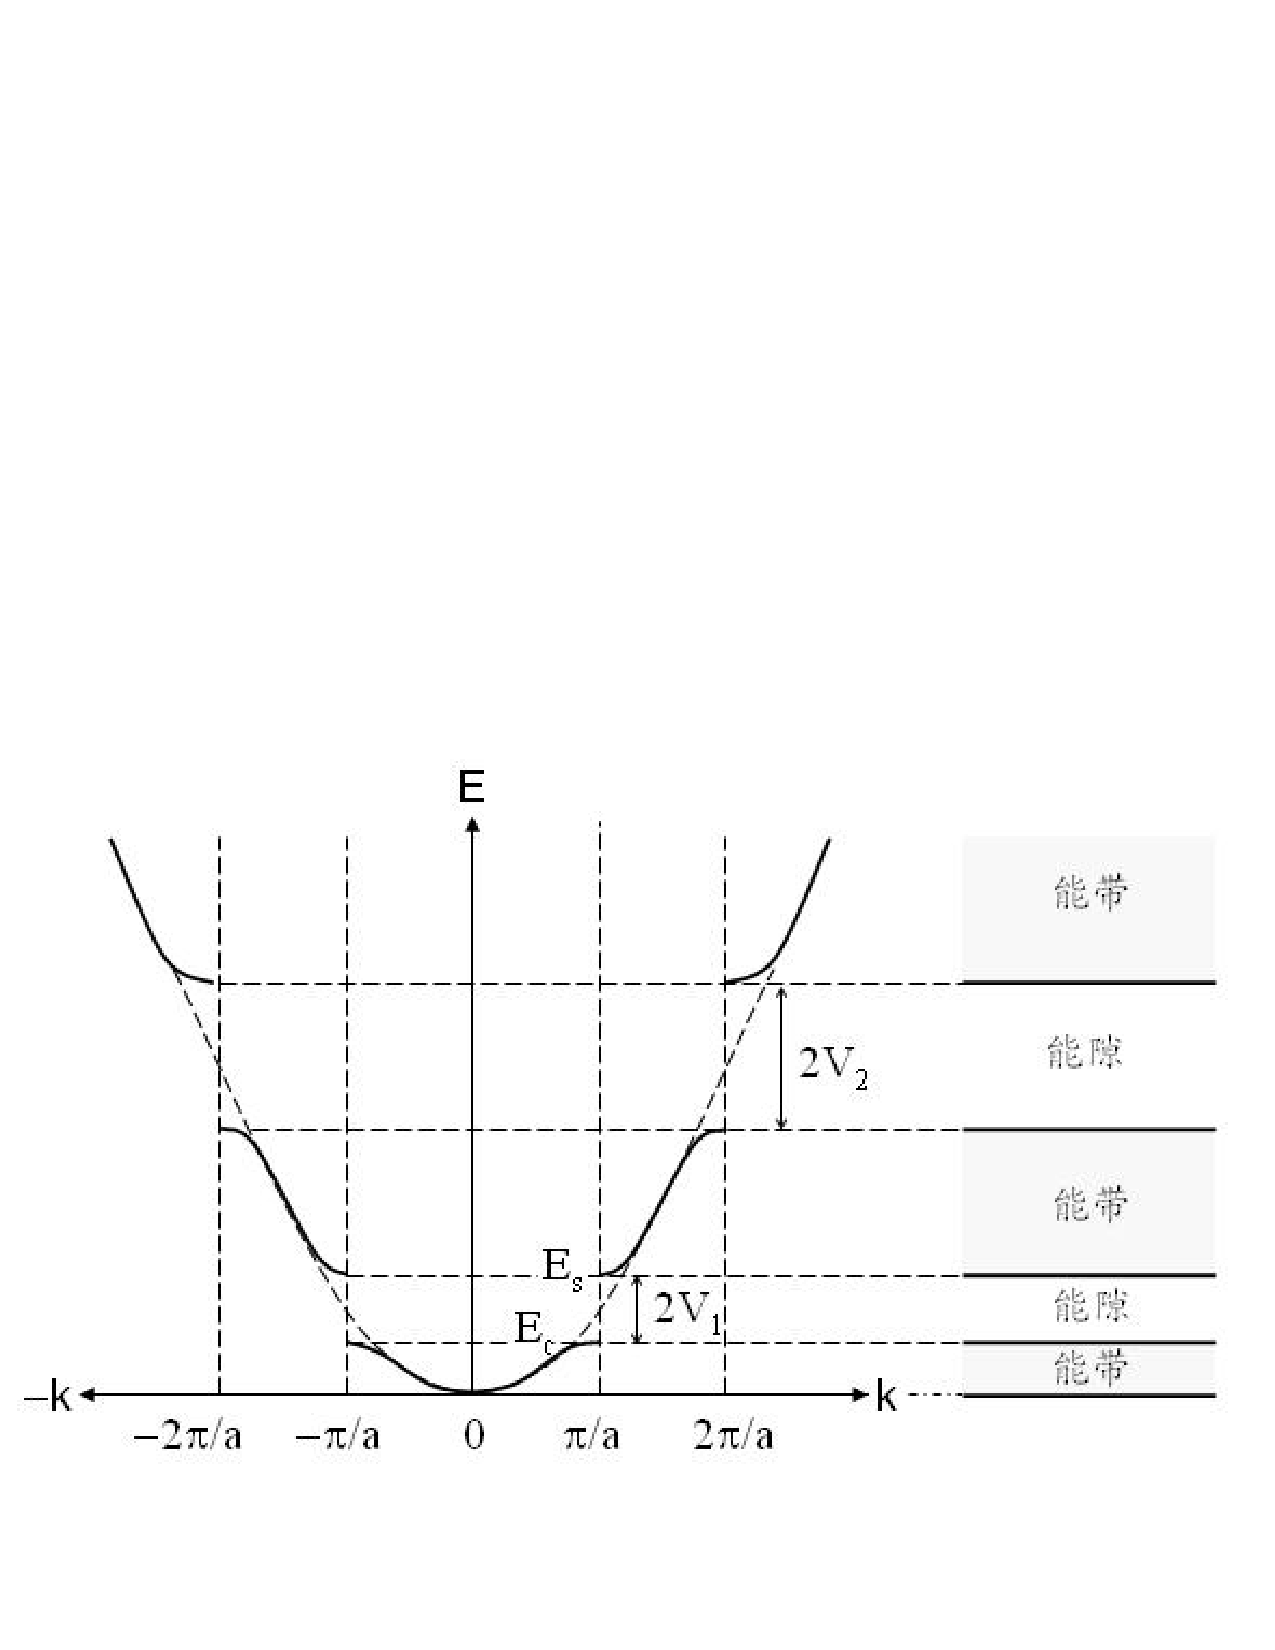
\includegraphics[height=2.1in,width=3.8in,viewport=10 90 570 380,clip]{Figures/Band_Gap.pdf}
\caption{\tiny \textrm{The Band-structure from free-electron gas.}}%
\label{Band-Gap-co}
\end{figure} 
}

\frame
{
\frametitle{紧束缚模型}
从分子轨道到能带
\begin{figure}[h!]
\centering
\hspace*{-0.29in}
\vspace*{-0.1in}
\subfigure[一维$\mathrm{H}$原子链]{
\label{fig:Hydrogen-1D}
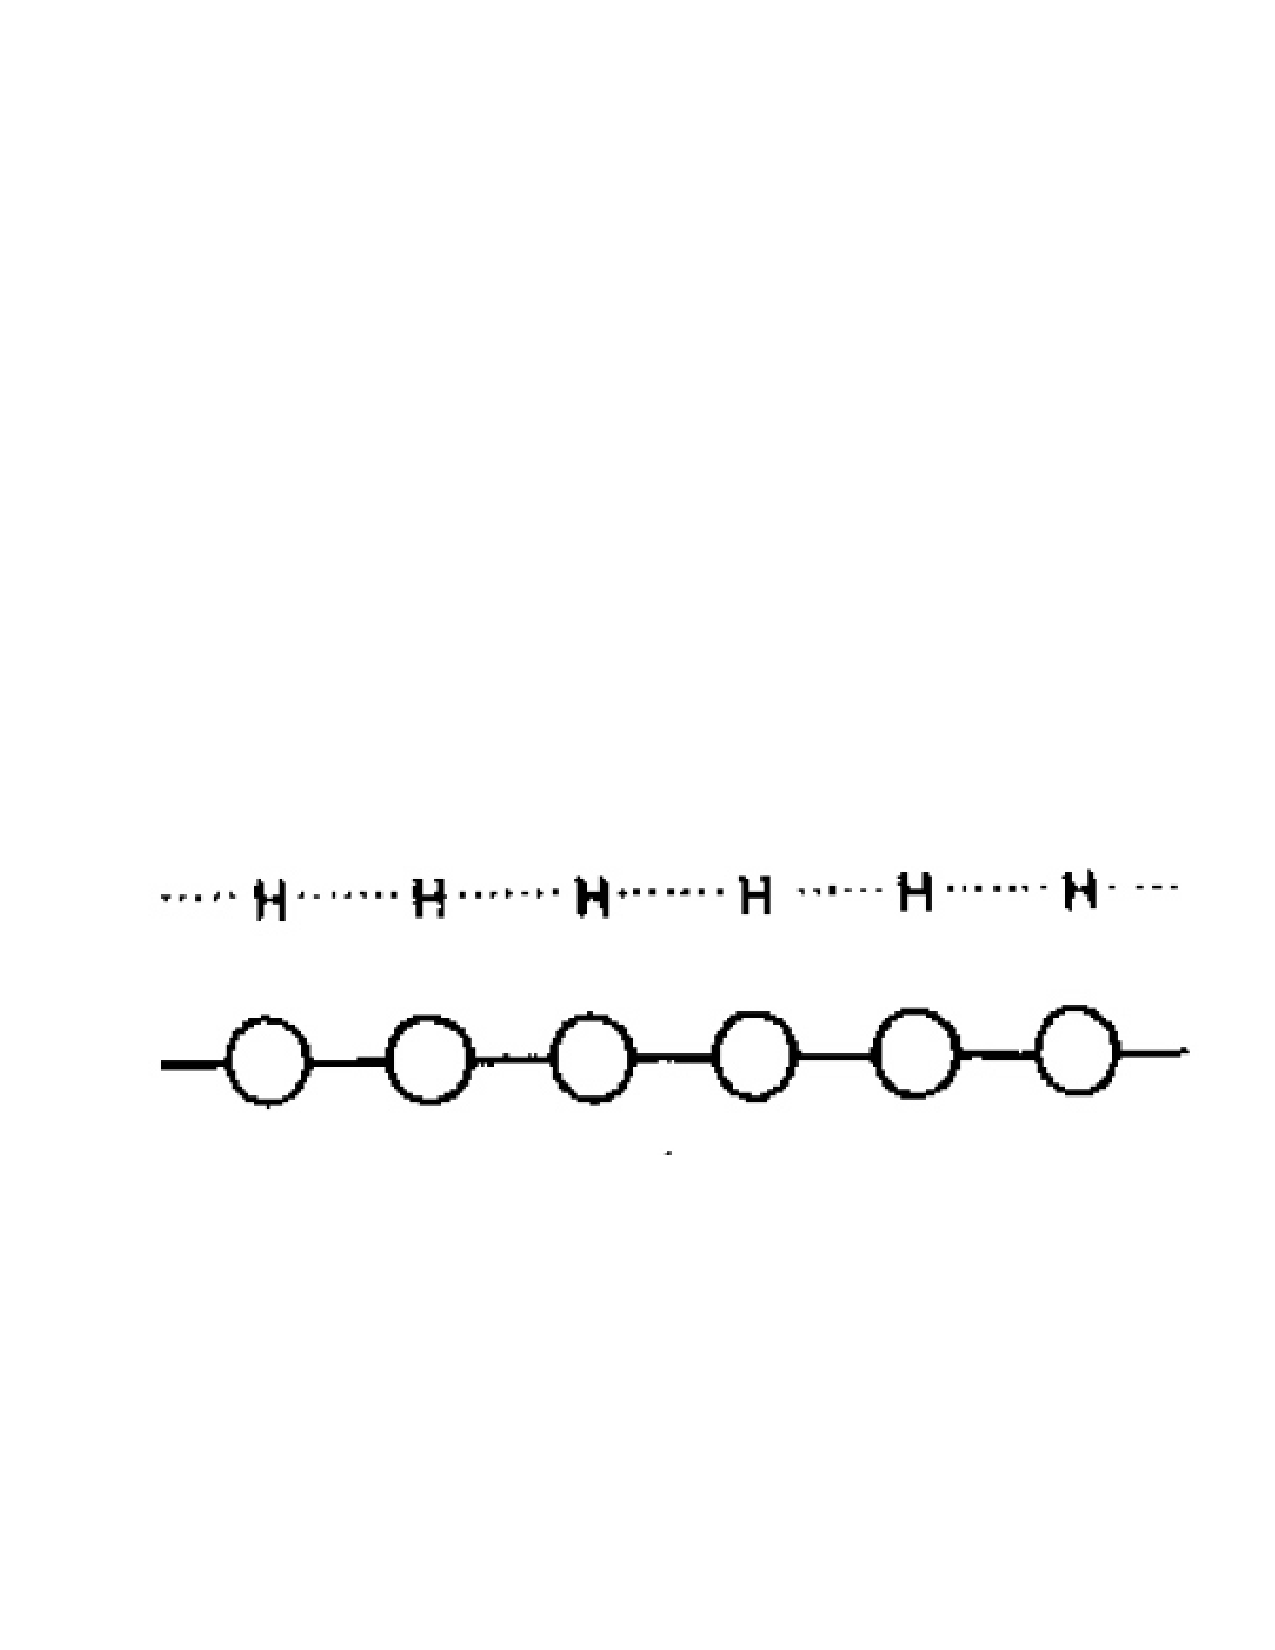
\includegraphics[height=0.25in,width=1.1in,viewport=70 255 570 375,clip]{Figures/Hydrogen-1D.pdf}}
\subfigure[$\mathrm{H}_n$分子轨道]{
\label{fig:Hydrogen-2-n}
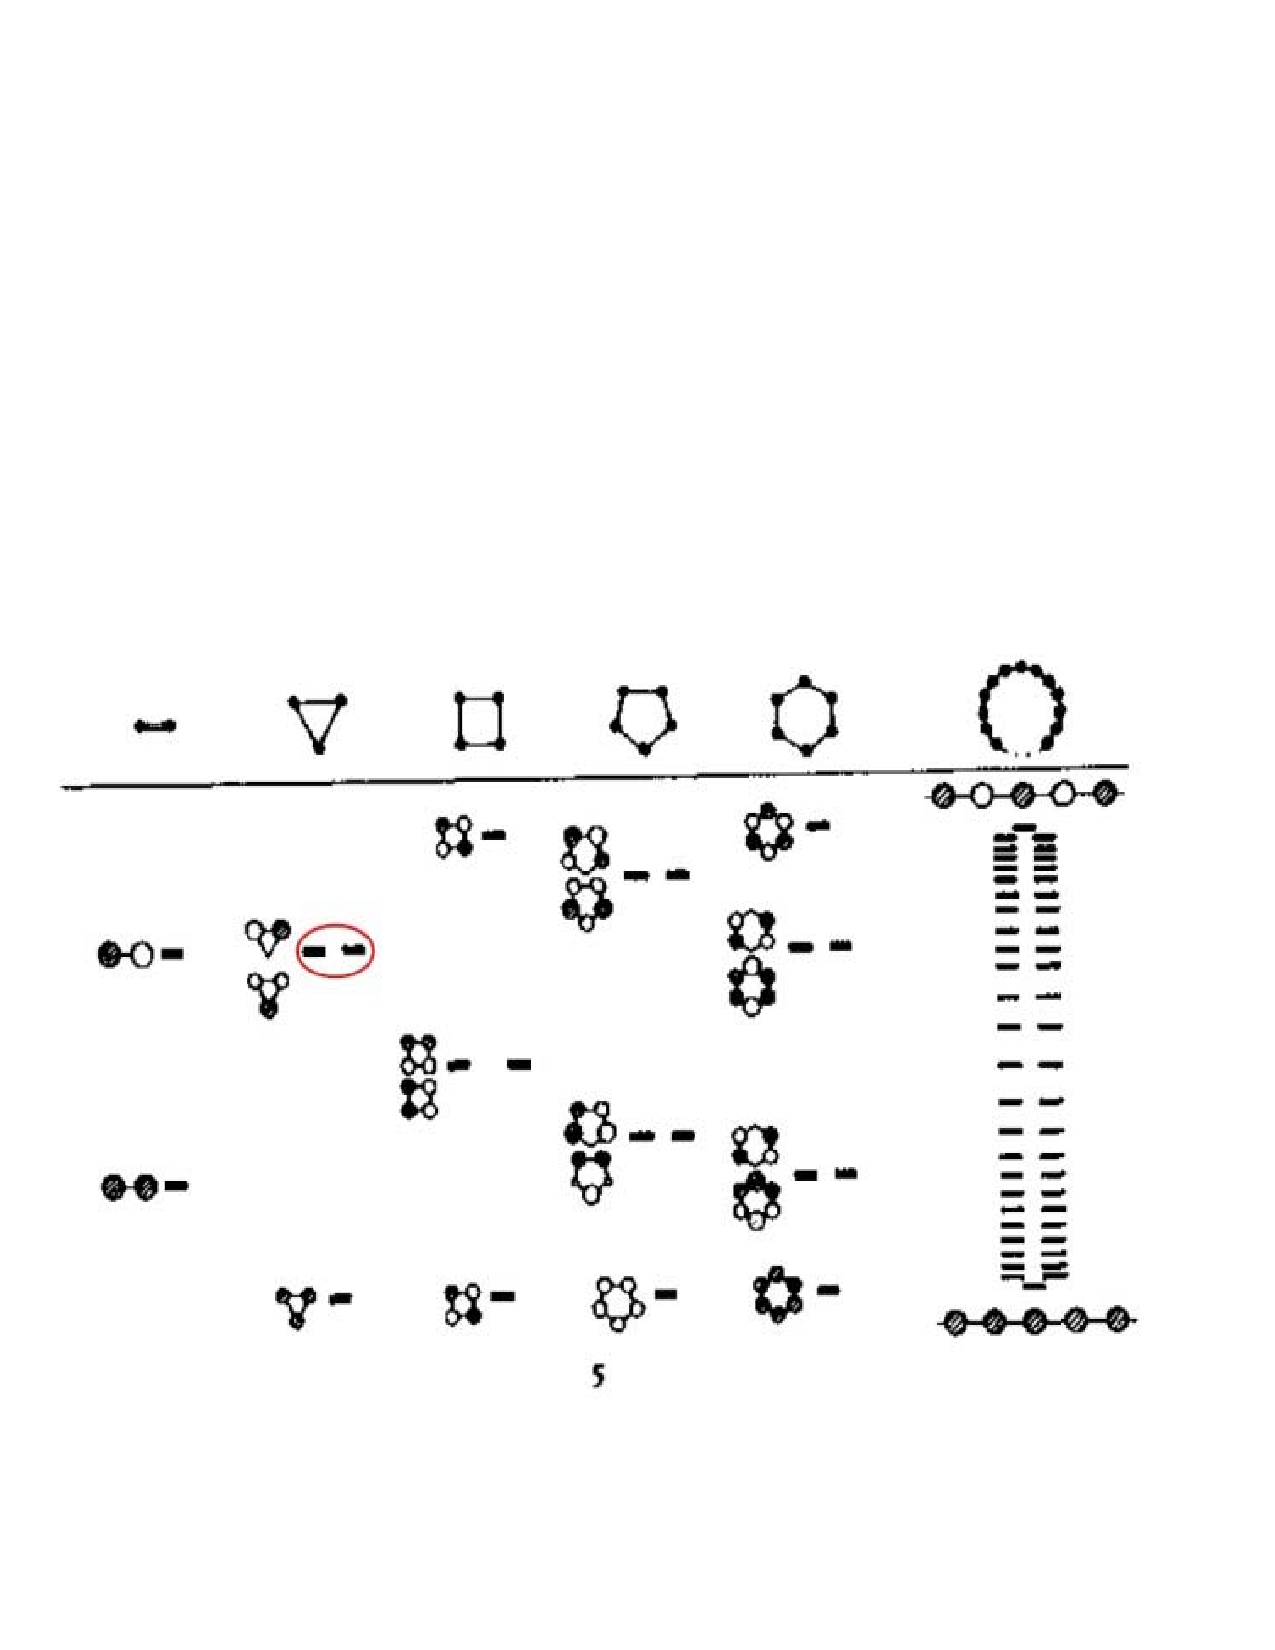
\includegraphics[height=0.8in,width=1.5in,viewport=30 140 545 480,clip]{Figures/Hydrogen-Mol-Orbital.pdf}}
\subfigure[分子波函数]{
\label{fig:Hydrogen-Psi}
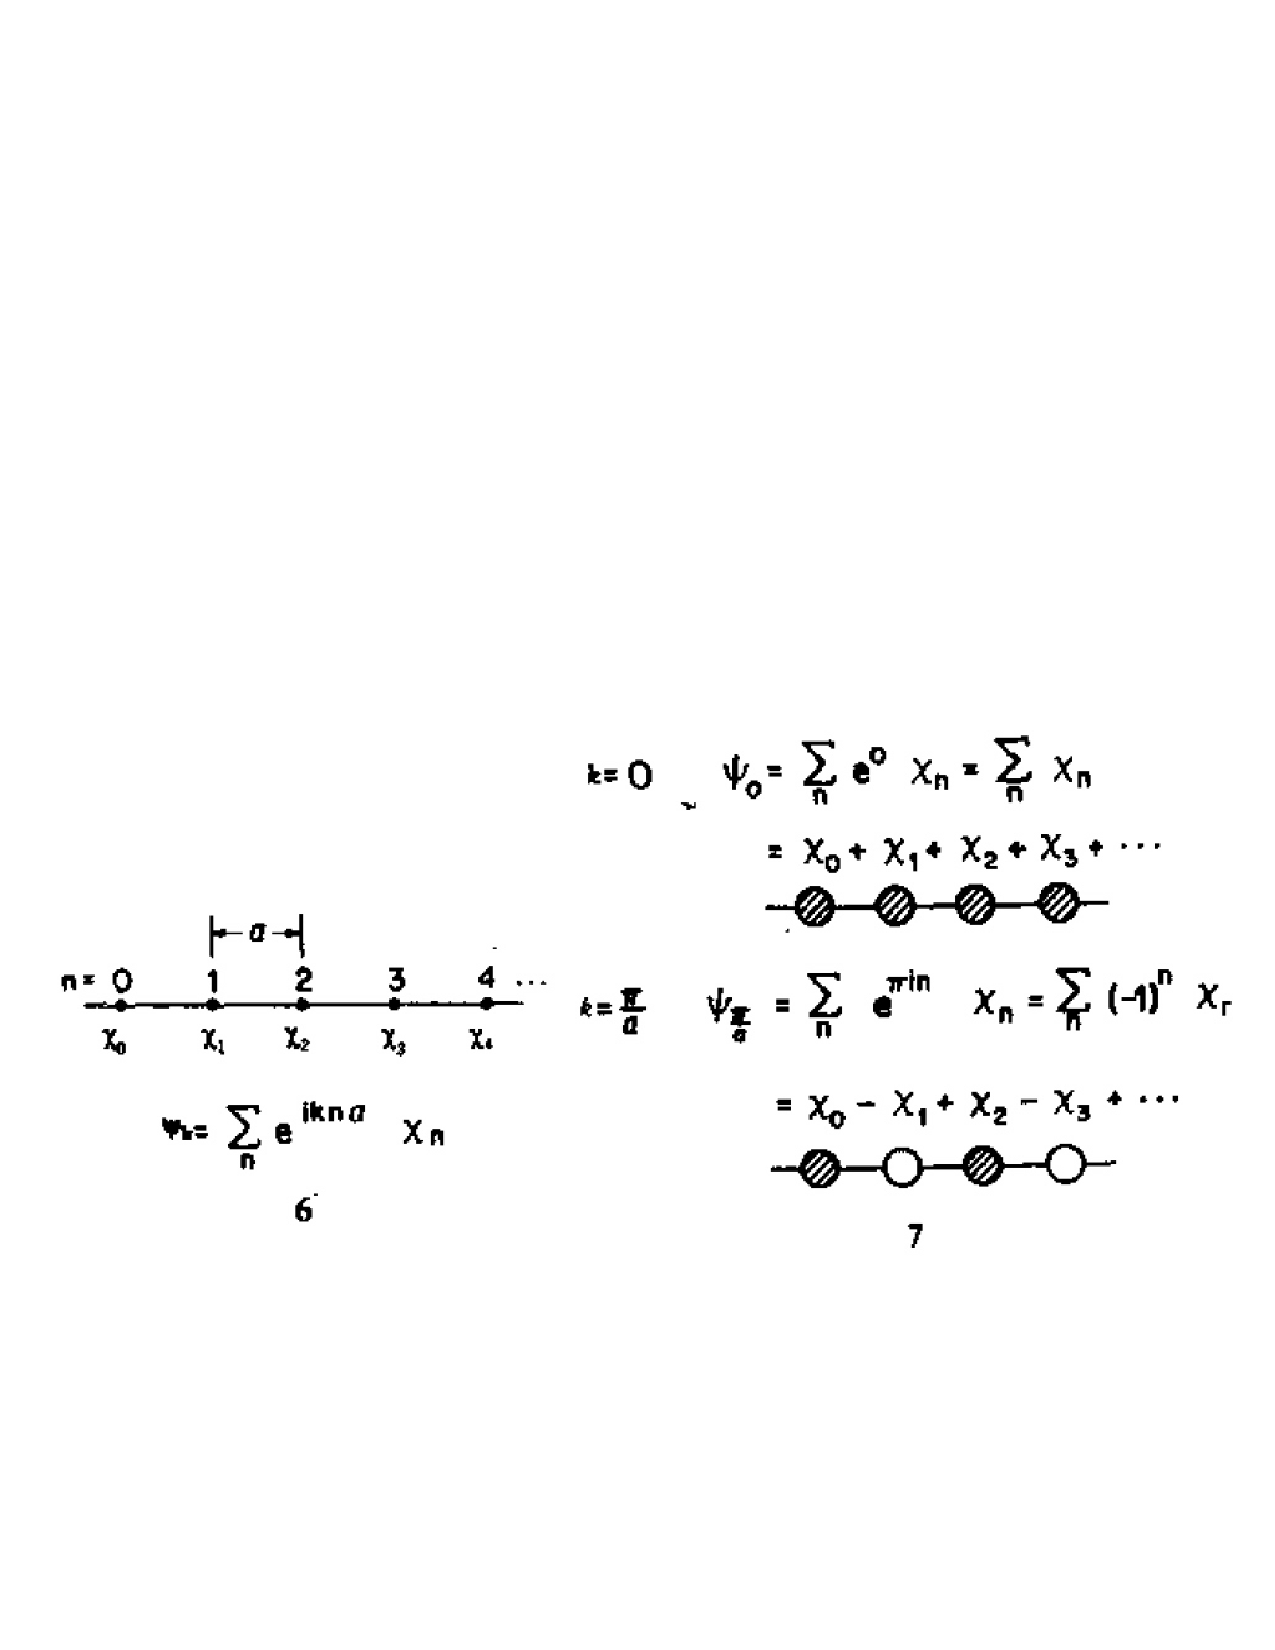
\includegraphics[height=0.5in,width=1.4in,viewport=25 218 595 440,clip]{Figures/Hydrogen-Psi.pdf}}\\
\vspace*{5pt}
\subfigure[分子轨道与能带]{
\label{fig:Hydrogen-Band-1D}
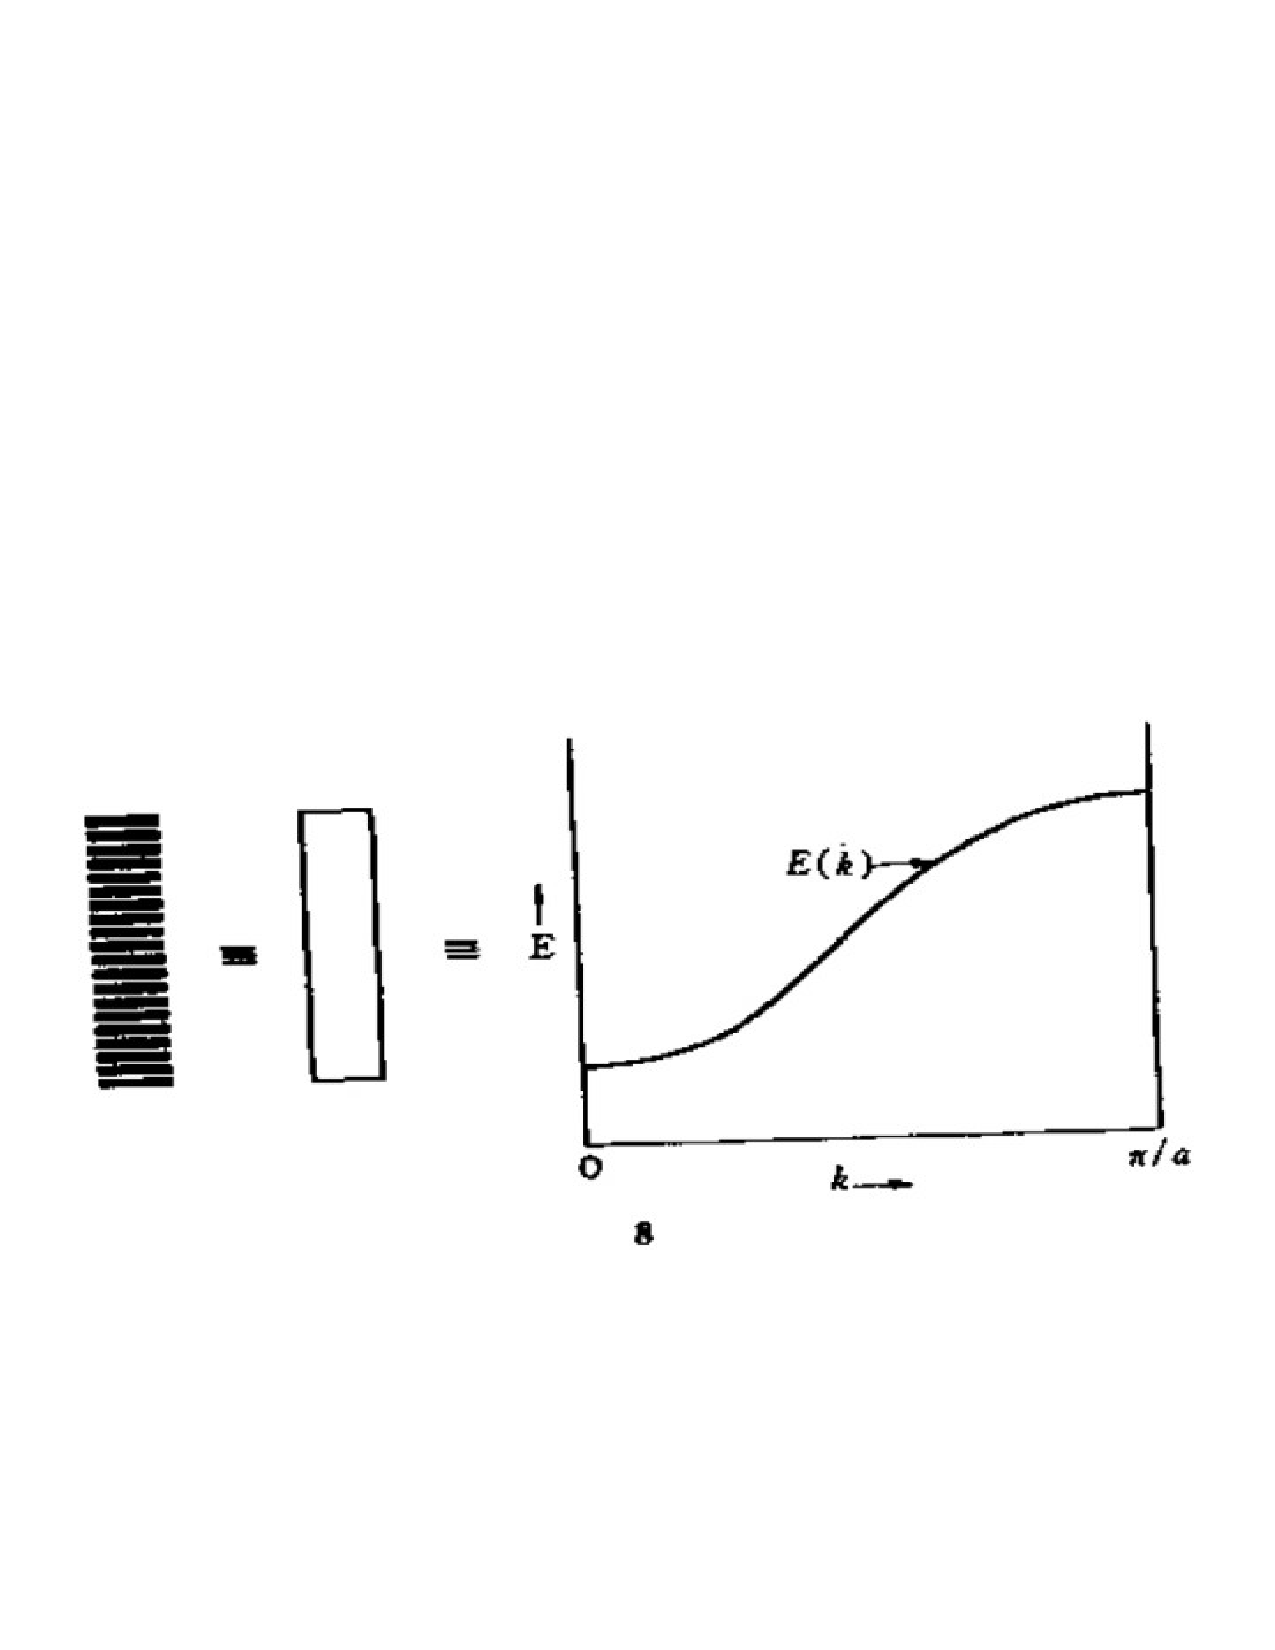
\includegraphics[height=0.6in,width=1.4in,viewport=35 215 575 450,clip]{Figures/Hydrogen-Band-1D.pdf}}
\subfigure[$d$\,轨道]{
\label{fig:Hydrogen-d-Band-1D}
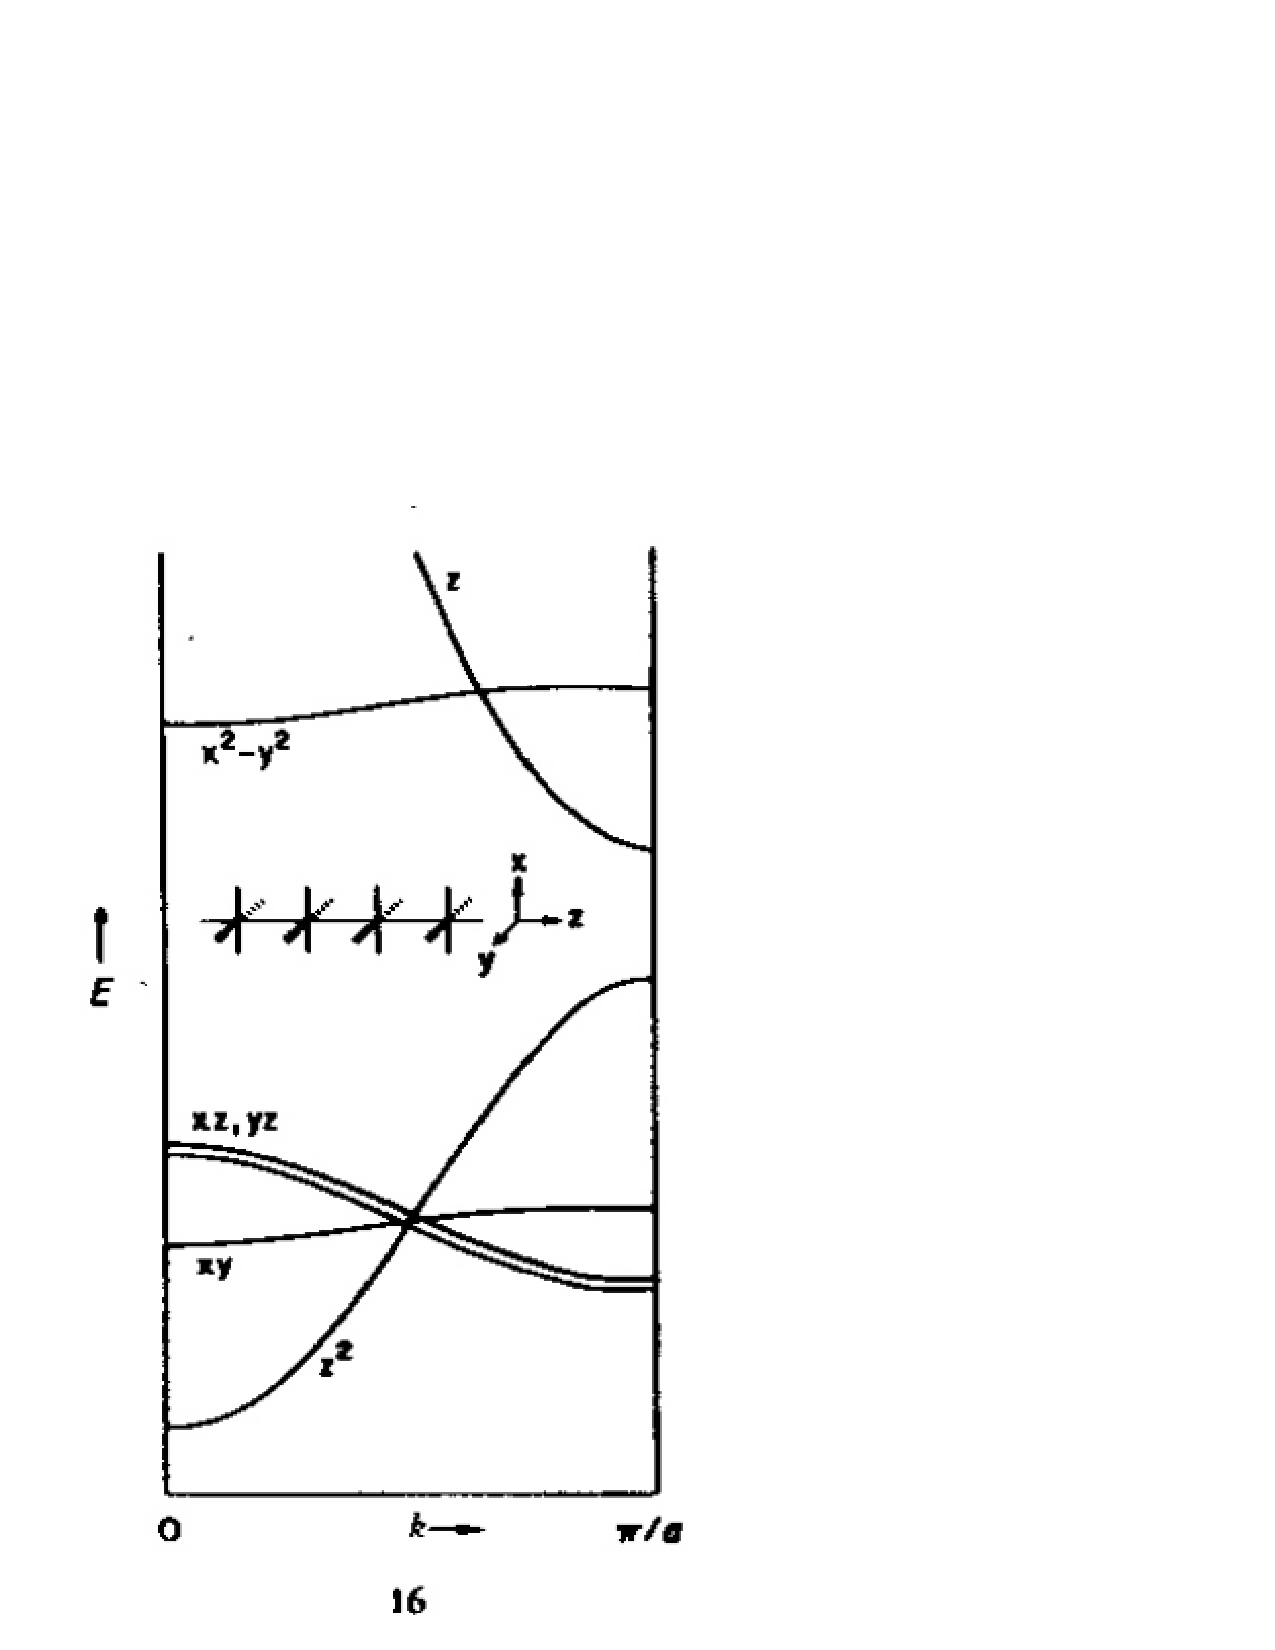
\includegraphics[height=1.0in,width=0.7in,viewport=40 45 330 535,clip]{Figures/Hydrogen-d-Band-1D.pdf}}
\caption{\tiny \textrm{The Band-structure from Molecular-orbital.}}%
\label{Band-Structure-local-orbit}
\end{figure} 
}

\subsection{能带、$\vec k$-空间与~\rm{Fermi~}面}
\frame
{
\frametitle{能带、$\vec k$空间与\textrm{Fermi}面}
\vspace{30pt}
\begin{figure}[h!]
\centering
\hspace*{-0.10in}
\subfigure[\textrm{Band structure}]{
\label{Band_Gap_Fermi-1}
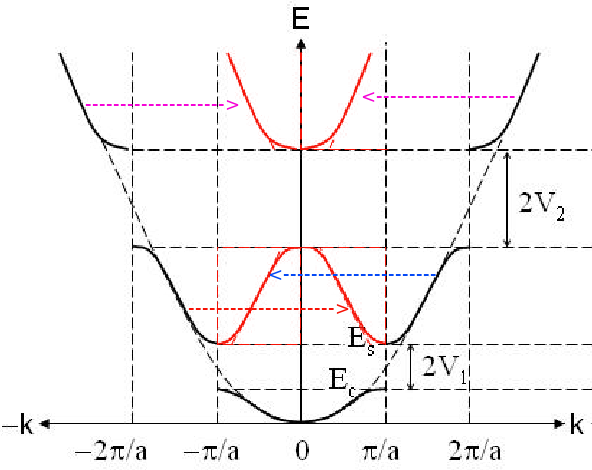
\includegraphics[height=1.6in,width=2.1in,viewport=0 0 480 350,clip]{Figures/Band_Brillouin_zone.png}}
\subfigure[\textrm{Brillouin Zone}]{
\label{Band_Gap_Fermi-2}
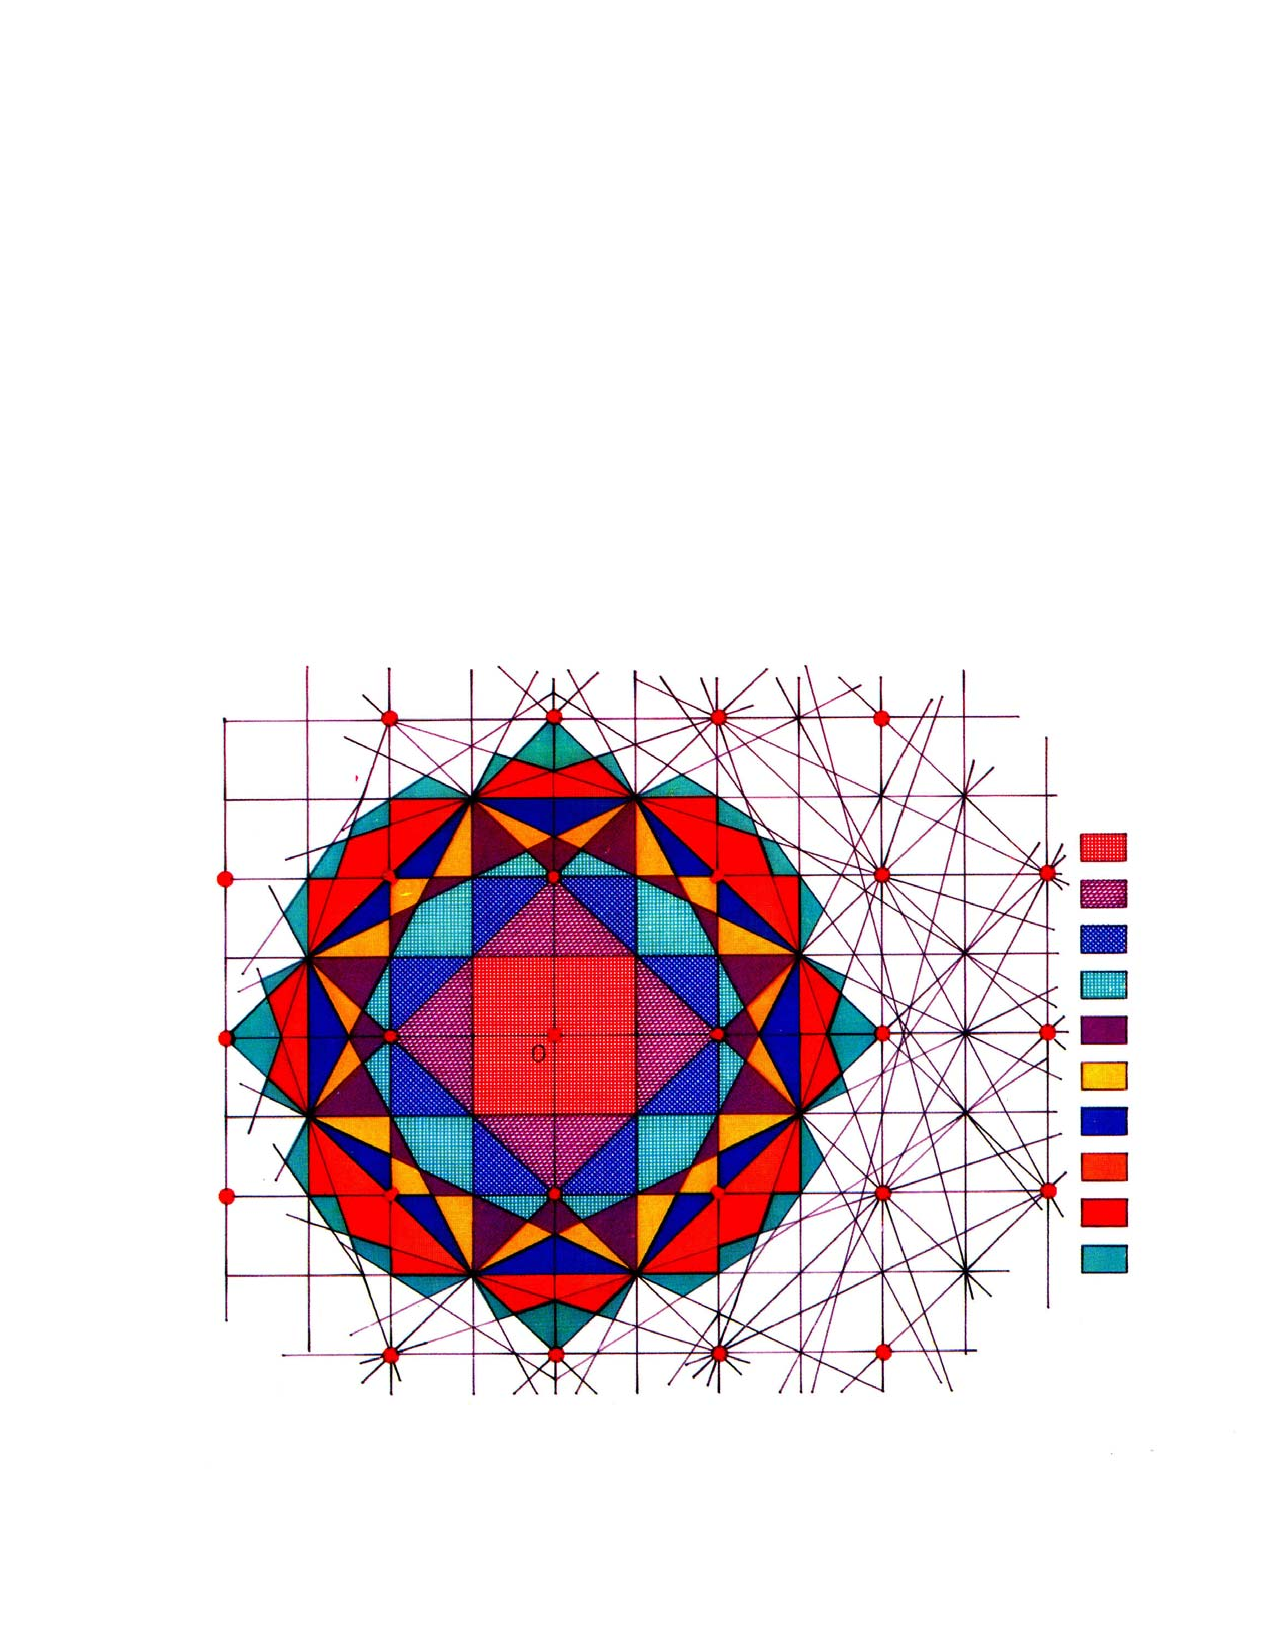
\includegraphics[height=1.28in,width=1.75in,viewport=100 120 545 470,clip]{Figures/2D_Brillouin-Zone.pdf}}
\label{Band_Gap_Fermi}
\end{figure}
}

\frame
{
	\frametitle{简单立方体系的\textrm{Brillouin}区与能带}
\vspace{10pt}
\begin{figure}[h!]
\centering
\hspace*{-0.28in}
\subfigure[\textrm{Brillouin Zone of Cubic lattice}]{
\label{Brillouin_Zone_Cubic-1}
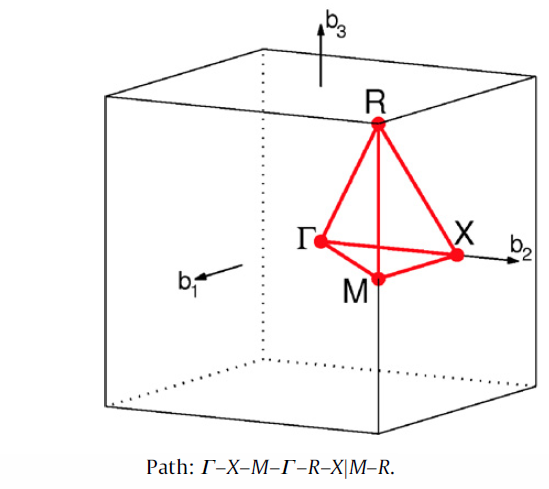
\includegraphics[height=2.1in,width=2.0in,viewport=90 0 550 500,clip]{Figures/Brillouin-Zone_CUB.png}}
\subfigure[\textrm{Band Structure of \ch{SrSnO3}}]{
\label{Band_Gap_SrSnO3-1}
\vspace*{-1.00in}
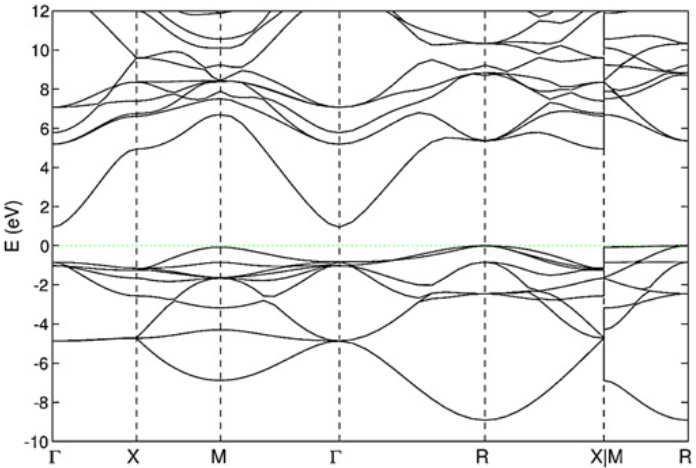
\includegraphics[height=2.10in,width=1.75in,viewport=0 0 710 550,clip]{Figures/Band-Struct_SrSnO3.png}}
\label{Band_Gap_CUB_SrSnO3}
\end{figure}
}

\frame
{
	\frametitle{面心立方体系的\textrm{Brillouin}区与能带}
\vspace{10pt}
\begin{figure}[h!]
\centering
\hspace*{-0.30in}
\subfigure[\textrm{Brillouin Zone of FCC lattice}]{
\label{Brillouin_Zone_FCC}
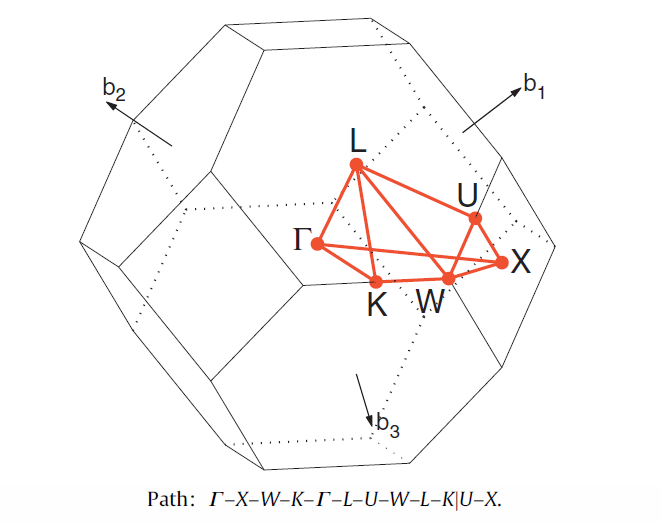
\includegraphics[height=1.9in,width=1.8in,viewport=75 0 560 520,clip]{Figures/Brillouin-Zone_FCC.png}}
\subfigure[\textrm{Band structure of \ch{CdS}}]{
\label{Band_Gap_CdS}
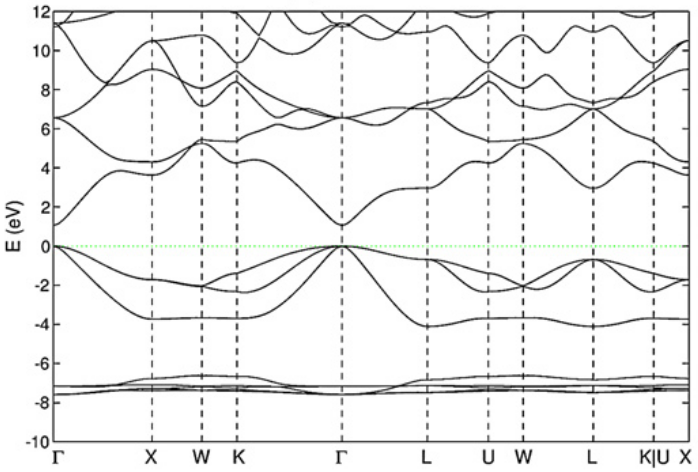
\includegraphics[height=2.10in,width=1.95in,viewport=0 0 700 520,clip]{Figures/Band-Struct_CdS.png}}
\label{Band_Gap_FCC_CdS}
\end{figure}
}

\frame
{
	\frametitle{体心立方体系的\textrm{Brillouin}区与能带}
\vspace{10pt}
\begin{figure}[h!]
\centering
\hspace*{-0.30in}
\subfigure[\textrm{Brillouin Zone of BCC lattice}]{
\label{Brillouin_Zone_BCC}
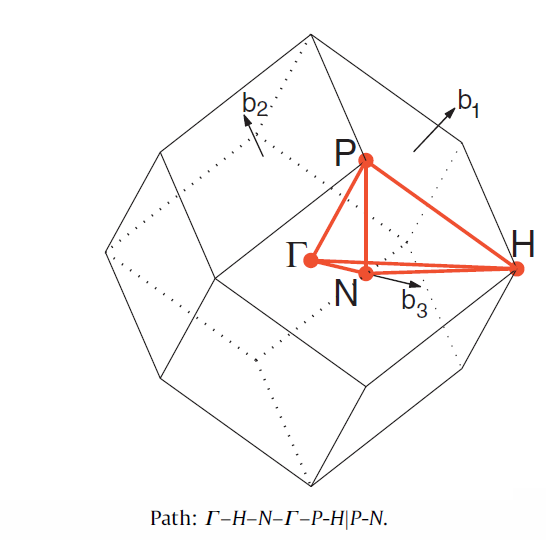
\includegraphics[height=2.1in,width=1.9in,viewport=80 0 550 520,clip]{Figures/Brillouin-Zone_BCC.png}}
\subfigure[\textrm{Band structure of \ch{GeF4}}]{
\label{Band_Gap_GeF4}
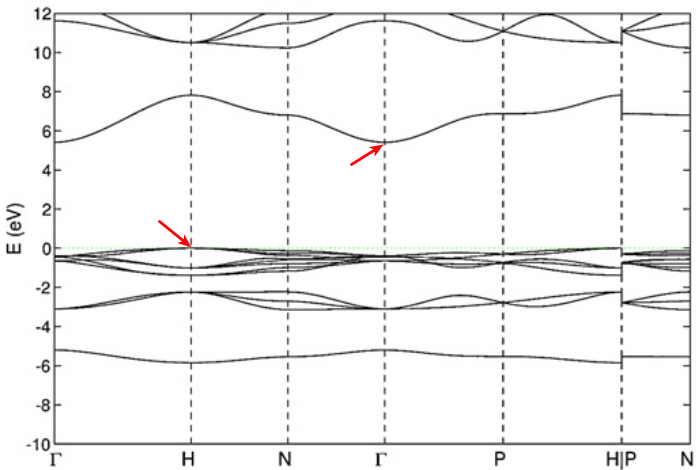
\includegraphics[height=2.10in,width=1.95in,viewport=0 0 700 500,clip]{Figures/Band-Struct_GeF4.png}}
\label{Band_Gap_BCC_GeF4}
\end{figure}
}

\subsection{固体能带计算方法}
\frame
{
%\frametitle{The methods on band structure calculation}
\frametitle{固体能带计算方法}
%\vskip 10pt
%\textrm{The mainly difference of all these methods below: the basis sets and the construction of the potential}
\vskip 10pt
常用的计算方法
\begin{itemize}%[+-| alert@+>]
%\begin{enumerate}%[+-| alert@+>]
\setlength{\itemsep}{12pt}
%  \item \textrm{Plane wave and the pseudo-potential}
	\item	平面波方法
	\item	正交平面波\textrm{(The orthogonalized plane wave, OPW)}和赝势\textrm{(Pseudo-potential, PP)}方法\upcite{Singh,PRB41-7892_1990,JPCM6-8245_1994}
	\item	缀加平面波\textrm{(Augmented plane wave, APW)}方法
	\item	\textrm{MT}轨道\textrm{(Muffin-tin orbitals, MTO)}方法
	\item	投影子缀加波\textrm{(Projector Augmented Wave, PAW)}方法\upcite{PRB50-17953_1994,PRB59-1758_1999}
\end{itemize}
\vskip 5pt 各种方法的\textcolor{red}{主要区别}:~\textcolor{blue}{势函数的处理}与\textcolor{blue}{所选基函数类型}不同
}

%\frame
%{
%	\frametitle{生活中最常用的基}
%\begin{figure}[h!]
%	\vspace{-9pt}
%\centering
%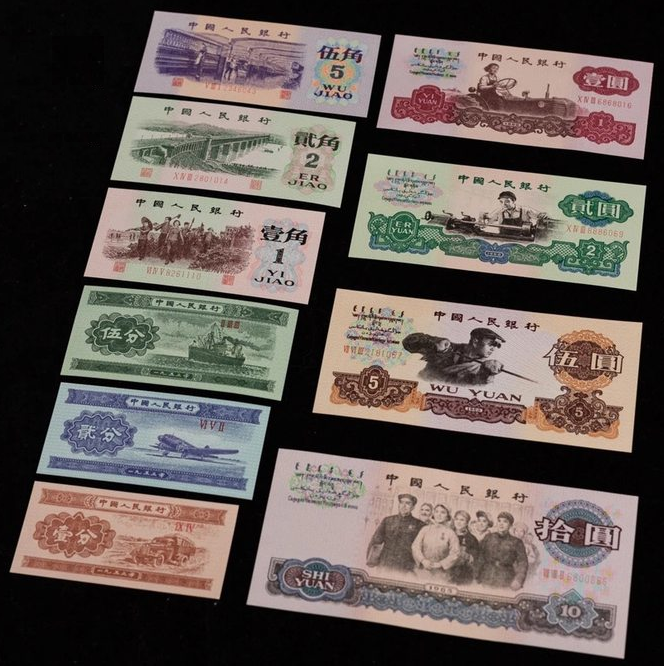
\includegraphics[height=2.70in,width=2.70in,viewport=0 0 160 160,clip]{Figures/Basis_set_example.png}
%\caption{\fontsize{5.5pt}{4.2pt}\selectfont{\textrm{第三套人民币(1962年4月20日起陆续发行,2000年7月1日停止流通).}}}%(与文献\cite{EPJB33-47_2003}图1对比)
%\label{Basic-set:Money}
%\end{figure}
%}
%
\frame
{
	\frametitle{多重散射理论}
\begin{figure}[h!]
	\vspace{-11pt}
\centering
\animategraphics[autoplay, loop, height=1.0in]{1}{Figures/Multi_scattering-}{0}{9}
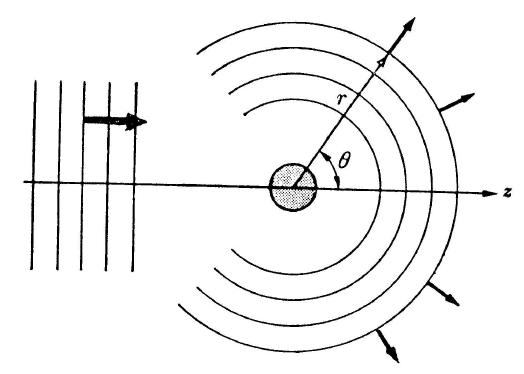
\includegraphics[height=1.29in,width=1.91in,viewport=0 0 400 275,clip]{Figures/Pseudo-scatter.jpg}
\caption{\fontsize{5.5pt}{4.2pt}\selectfont{\textrm{Schematic illustration of scattering of a plane wave by a spherical potential.}}}%(与文献\cite{EPJB33-47_2003}图1对比)
\label{Multiple_scattering}
\end{figure}
\vspace*{-0.10in}
\fontsize{7.5pt}{6.2pt}\selectfont{
	入射平面波用球\textrm{Bessel}函数展开
$$\mathrm{e}^{\mathrm{i}\vec q\cdot\vec r}=4\pi\sum_{lm}\mathrm{i}^lj_l(\vec q\cdot\vec r)Y_{lm}^{\ast}(\hat{\vec q})Y_{lm}(\hat{\vec r})=\sum_{l}(2l+1)\mathrm{i}^lj_l(qr)P_{l}(\cos\theta)$$
%$$\mathrm{e}^{\mathrm{i}\vec q\cdot\vec r}=\mathrm{e}^{\mathrm{i}qr\cos(\theta)}=\sum_{l}(2l+1)\mathrm{i}^lj_l(qr)P_{l}[\cos(\theta)]$$
}
}

\frame
{
	\frametitle{势阱与相移}
\begin{figure}[h!]
\centering
\vspace*{-0.26in}
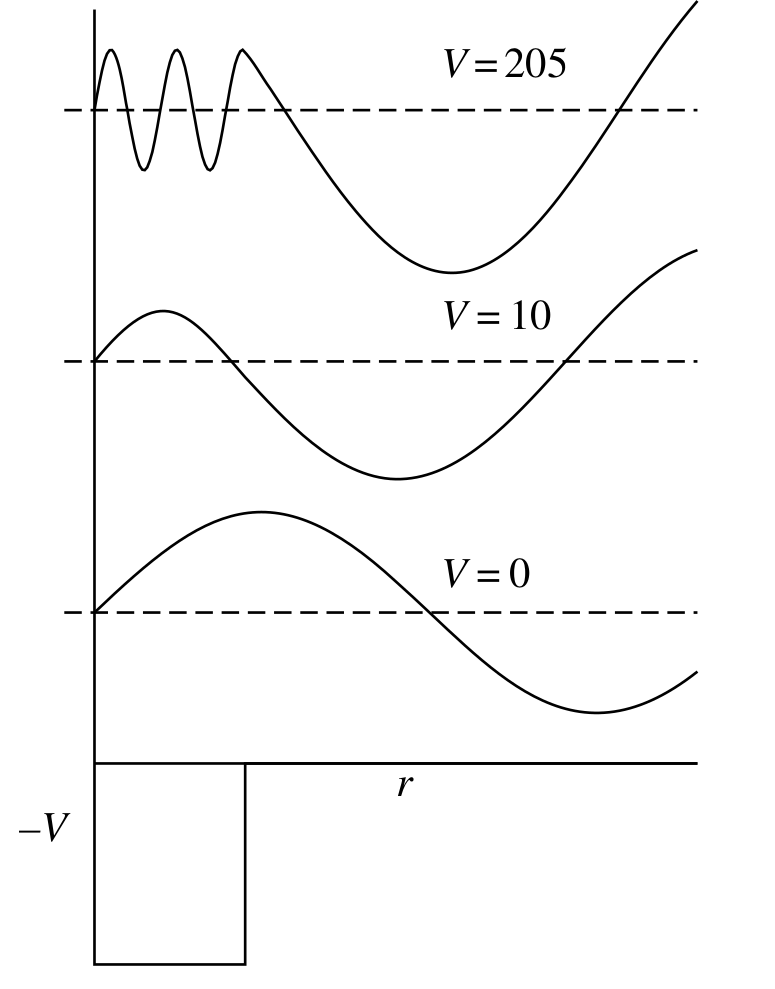
\includegraphics[height=1.85in,width=1.3in,viewport=0 0 750 1050,clip]{Figures/Radial_wave_functions_for_various_square_well_potential.png}
\caption{\fontsize{5.5pt}{4.2pt}\selectfont{\textrm{The radial wave functions for \textit{l}=0 for various square well potential depths.}}}%(与文献\cite{EPJB33-47_2003}图1对比)
\label{Pseudo-scatter}
\end{figure}
\vspace*{-0.1in}
\fontsize{7.5pt}{6.2pt}\selectfont{
平面波经散射后出射,波函数变为
$$\Psi_l^{>}(\varepsilon,r)=C_l\bigg[j_l(\kappa r)-\tan\eta_l(\varepsilon)n_l(\kappa r)\bigg]\quad\text{其中}\kappa^2=\varepsilon$$
根据散射理论,能量为$\varepsilon$的电子经单个势阱散射偏转$\theta$后,波函数的振幅可以表示为
	\begin{displaymath}
		t(\theta)=\dfrac{4\pi}{\kappa}\sum_l(2l+1)[\mathrm{exp}(2\mathrm{i}\eta_l(\varepsilon))-1]P_l(\cos\theta)
	\end{displaymath}
%$$t(\theta)=\dfrac{4\pi}{\sqrt\varepsilon}\sum_l(2l+1)\bigg[\mathrm{e}^{2\mathrm{i}\eta_l(\varepsilon)}-1\bigg]P_l(\cos\theta)$$
%$$\eta_l(\varepsilon)=p_l\pi+\delta_l(\varepsilon)$$
}
}

\frame
{
	\frametitle{球形势散射的相移与赝势}
\begin{figure}[h!]
\centering
\vspace*{-0.20in}
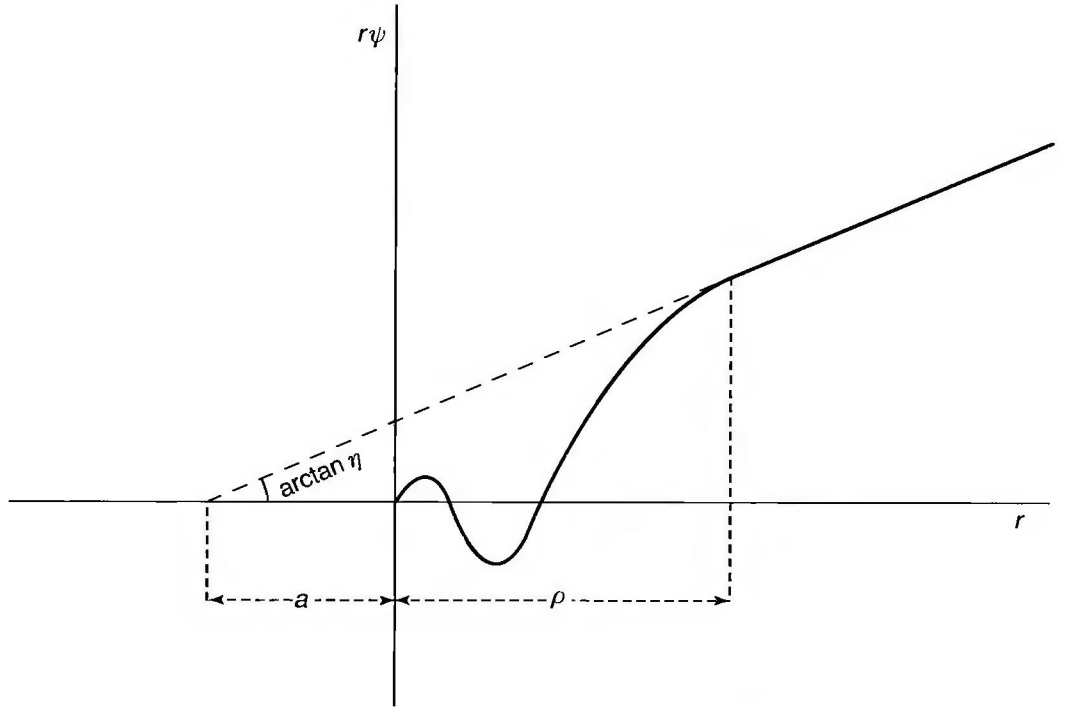
\includegraphics[height=1.20in,width=1.77in,viewport=0 0 1150 750,clip]{Figures/Pseudo-scatter-2.png}
\caption{\fontsize{4.5pt}{3.2pt}\selectfont{\textrm{Radial wave-function $\phi=r\psi$ for low-energy scattering as illustrated in a figure from the 1934 and 1935 papers of Fermi and coworkers for low-energy electron scattering from atoms and neutron scattering from nuclei. The node in the wave-function near the origin show that the potential is attractive and strong enough to have bound states. The cross-section for scattering from the localized potential is determined by the phase shift and is the same for weaker pseudo-potential with the same phase shift modulo $2\pi$.}}}%(与文献\cite{EPJB33-47_2003}图1对比)
\label{Pseudo-scatter-2}
\end{figure}
\fontsize{7.5pt}{6.2pt}\selectfont{
对于球形势散射,相移可由径向波函数计算
$$\tan\eta_l(\varepsilon)=\dfrac{R\frac{\mathrm{d}}{\mathrm{d}r}j_l(\kappa r)|_R-D_l(\varepsilon)j_l(\kappa R)}{R\frac{\mathrm{d}}{\mathrm{d}r}n_l(\kappa r)|_R-D_l(\varepsilon)n_l(\kappa R)}$$
$$\mbox{其中~}D_l(\varepsilon,r)\equiv r\psi_l^{\prime}(r)/\psi_l(r)=r\dfrac{\mathrm{d}}{\mathrm{d}r}\ln\psi_l(r)$$
同时相移与波函数节点的关系为:$$\eta_l(\varepsilon)=p_l\pi+\delta(\varepsilon)$$}
}

%\frame
%{
%\begin{figure}[h!]
%\centering
%\vskip -3pt
%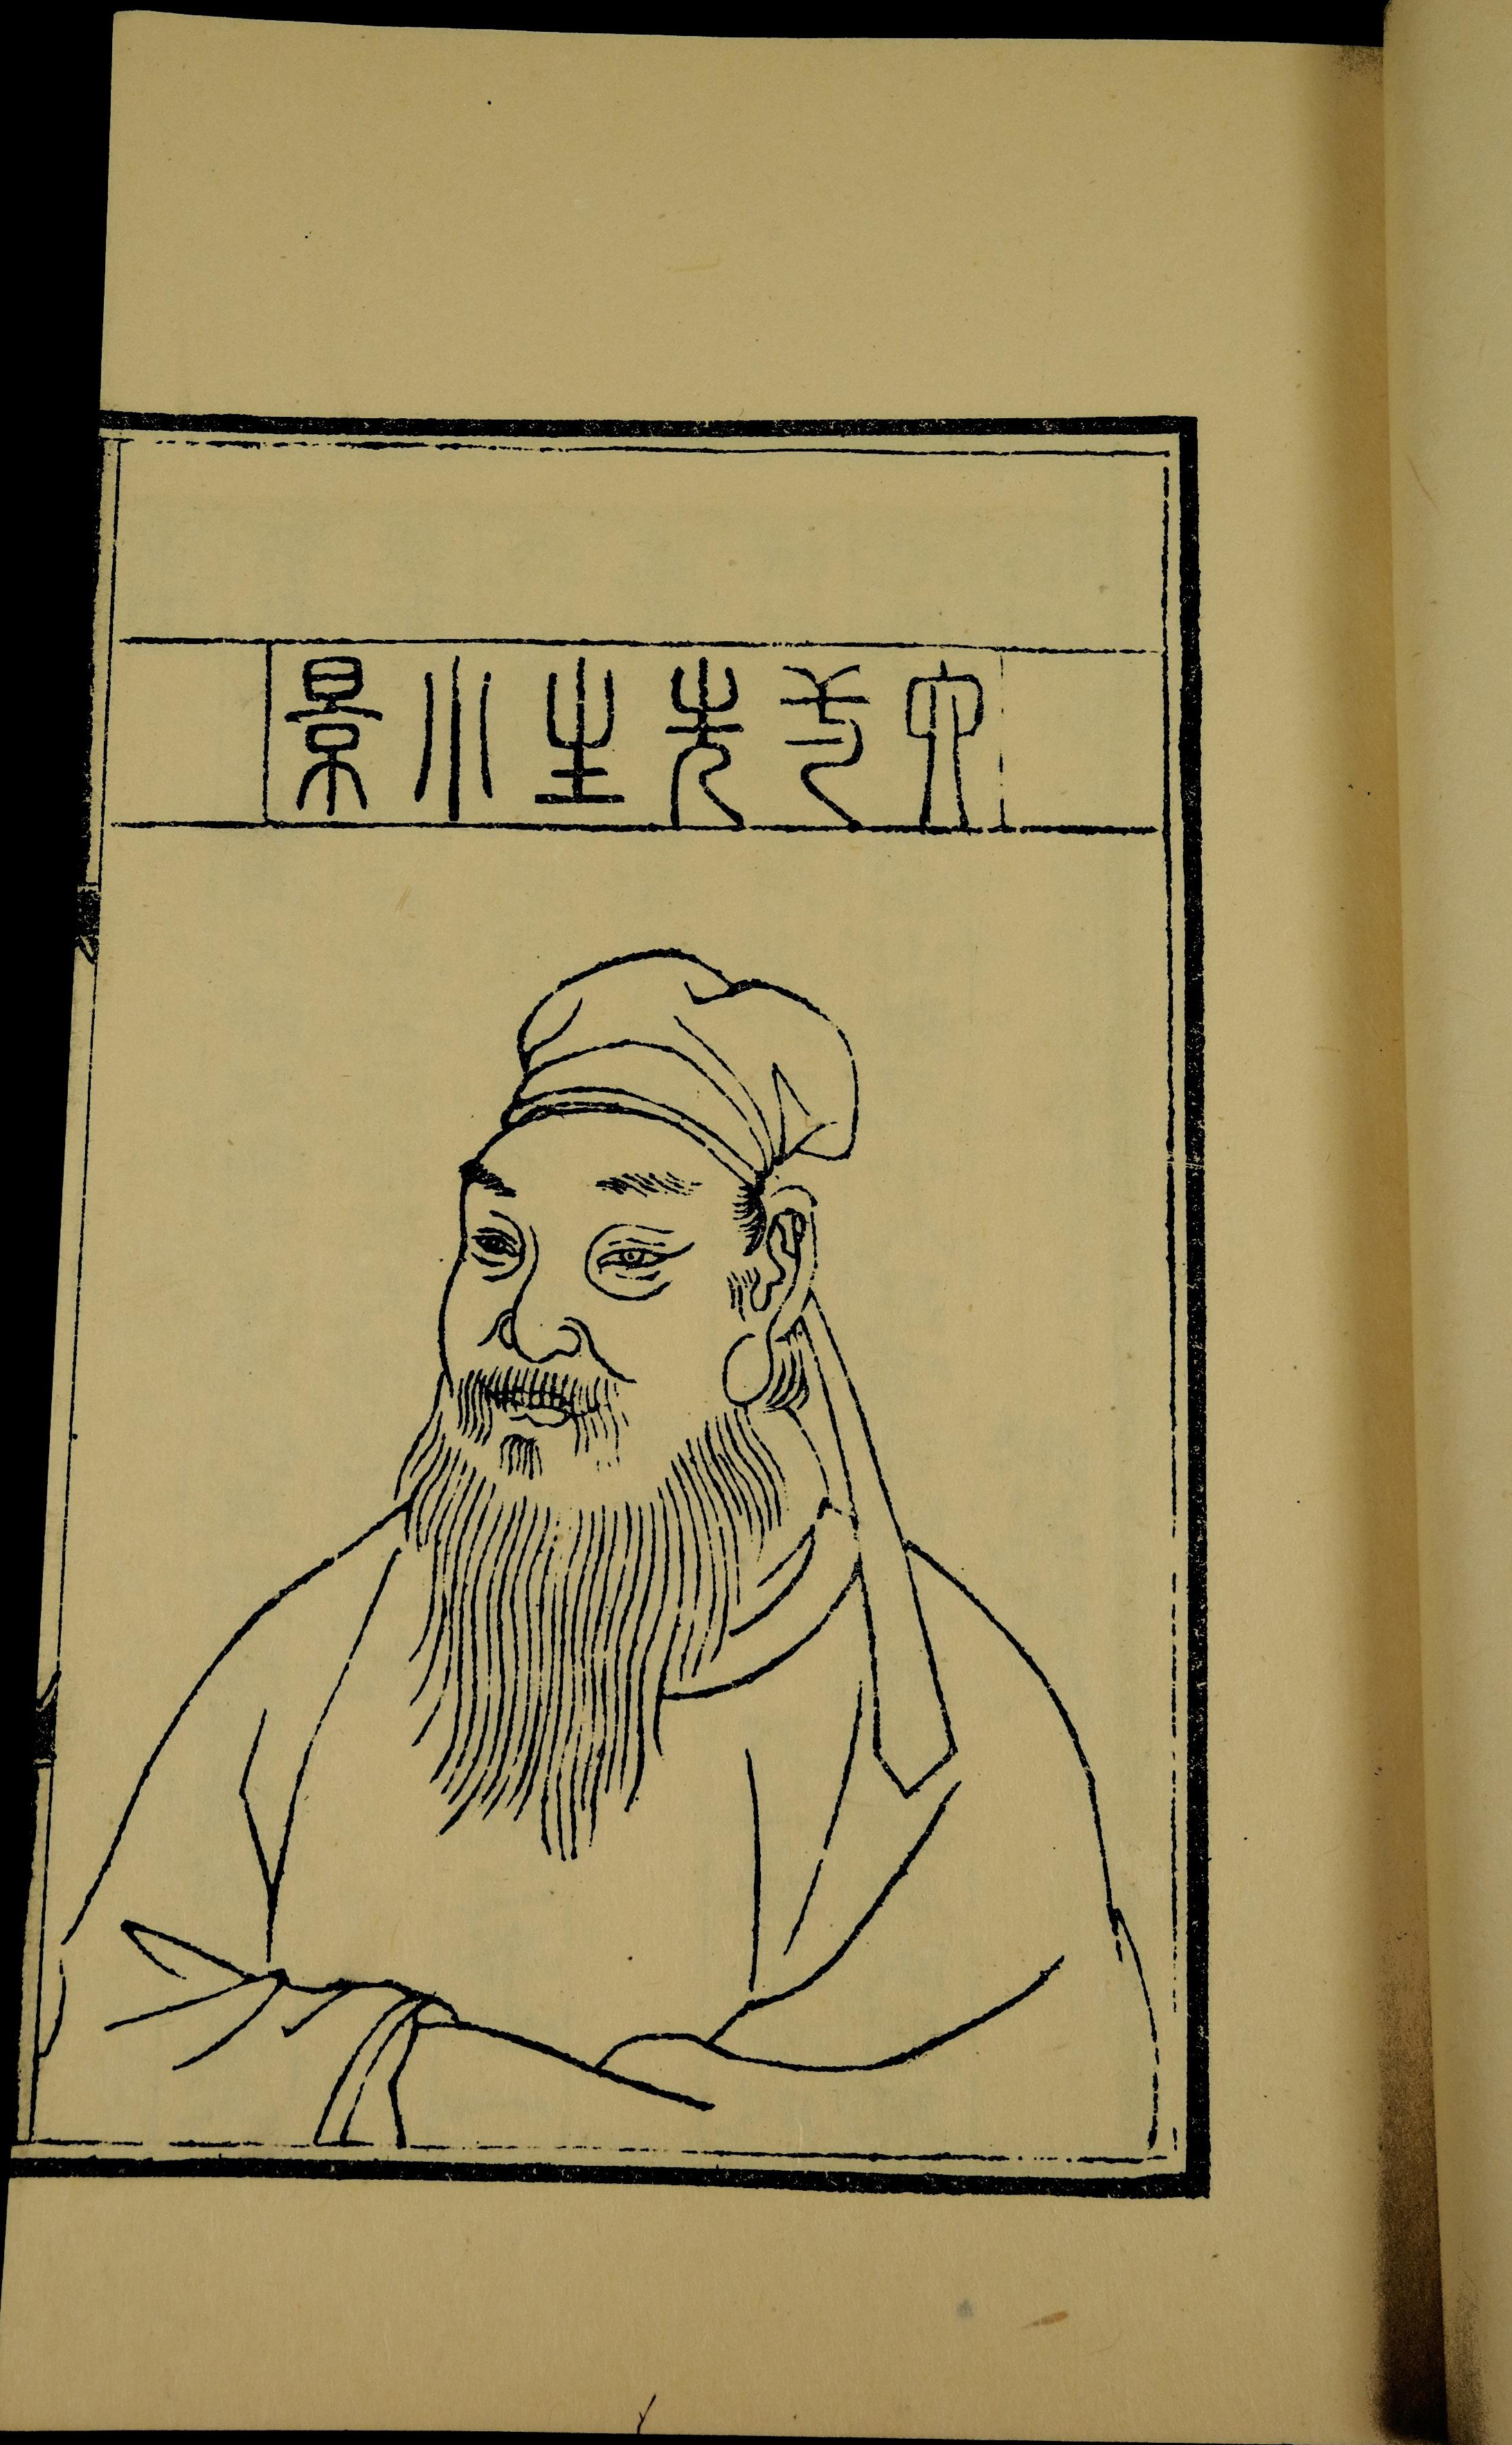
\includegraphics[height=2.5in,width=1.7in,viewport=0 0 600 850,clip]{Figures/Ouyang_Xiu-2.jpg}
%\hskip 20pt
%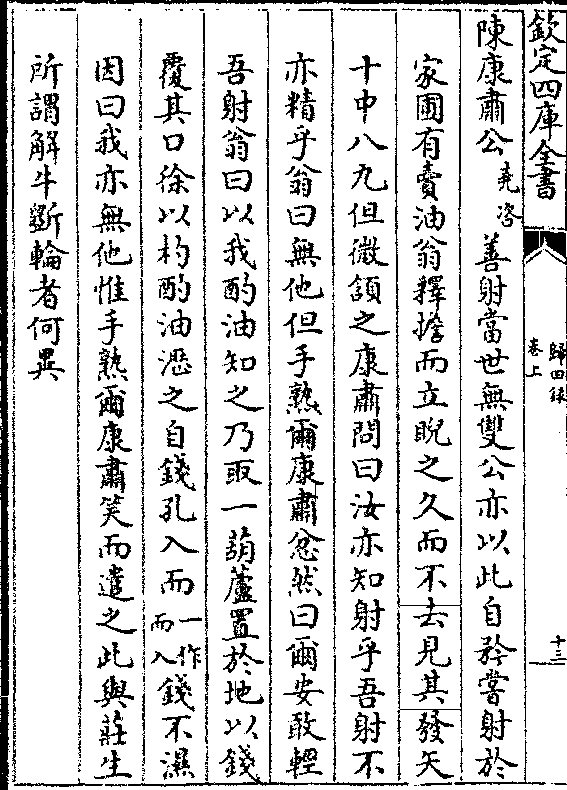
\includegraphics[height=2.5in,width=1.7in,viewport=0 0 600 790,clip]{Figures/Sale_Oil_Ouyang.png}
%\label{Sale_Oil_Ouyang}
%\caption{\tiny \textrm{欧阳修的《归田录\!$\cdot$\!卖油翁》.}}%(与文献\cite{EPJB33-47_2003}图1对比)
%\end{figure}
%}
%
%-----------------------------------------------------------------------------------------------------------------------------------------------------------------------%
\section{赝势理论}       %Bookmark
%\section{Induction on DFT and solid-state physics}       %Bookmark
\frame
{
%\frametitle{The methods on band structure calculation}
	\frametitle{由\textrm{OPW~}到赝势}
%\vskip 10pt
%\textrm{The mainly difference of all these methods below: the basis sets and the construction of the potential}
\begin{itemize}
%\setlength{\itemsep}{5pt}
	\item 完全平面波基组\\{\fontsize{7.5pt}{5.5pt}\selectfont{少数平面波就可以很好地描述波函数在原子间的行为,近核波函数则需要大量平面波展开}}%。因此完全平面波基组虽然方便,但求体系本征态对角化的矩阵非常巨大,计算变得异常耗时。
	\item 正交平面波(\textrm{Orthogonalized plane wave, OPW})方法\\{\fontsize{7.5pt}{5.5pt}\selectfont{价电子用与芯层波函数正交的平面波展开
		\begin{displaymath}
			\phi_{\textrm{OPW}}^{\vec k+\vec G}(\vec r)=\phi_{\textrm{PW}}^{\vec k+\vec G}(\vec r)-\sum_c\langle\varphi_c|\phi_{\textrm{PW}}^{\vec k+\vec G}\rangle\varphi_c(\vec r)
		\end{displaymath}}}
	{\fontsize{7.5pt}{5.5pt}\selectfont{构造赝波函数
		\begin{displaymath}
			\tilde{\phi}_v(\vec r)=\phi_v(\vec r)+\sum_c\langle\varphi_c|\tilde{\phi}_v\rangle\varphi_c(\vec r)
		\end{displaymath}
	代入\textrm{Schr\"odinger}方程
		$$\hat H|\tilde{\phi}_v\rangle-\sum_c\langle\varphi_c|\tilde{\phi}_v\rangle\hat H|\varphi_c\rangle=\varepsilon_v|\tilde{\phi}_v\rangle-\varepsilon_v\sum_c\langle\varphi_c|\tilde{\phi}_v\rangle|\varphi_c\rangle$$
		可有$$\hat H|\tilde{\phi}_v\rangle+\textcolor{blue}{V^R}|\tilde{\phi}_v\rangle=\textcolor{blue}{\varepsilon_v}|\tilde{\phi}_v\rangle$$
		这里排斥势是$$V^R(\vec r,\vec r^{\prime})=\sum_c(\varepsilon_v-\varepsilon_c)|\varphi_c(\vec r^{\prime})\rangle\langle\varphi_c(\vec r)|$$}}
\end{itemize}
}

\frame
{
	\frametitle{由\textrm{OPW~}到赝势}
	\textrm{Phillips-Kleinman}指出,赝势($V^{e\!f\!f}$)-赝波函数(可用$\phi_{PW}^{\vec k+\vec G}$展开)满足\textrm{Schr\"odinger}方程%\upcite{PR116-287_1959}
	$$\bigg(-\dfrac12\nabla^2+\textcolor{red}{V^{e\!f\!f}}\bigg)|\tilde{\phi}_v\rangle=\textcolor{blue}{\varepsilon_v}|\tilde{\phi}_v\rangle$$
	其中$\textcolor{red}{V^{e\!f\!f}}=V(\vec r)+\textcolor{blue}{V^R}$
	\begin{itemize}
		\item 赝势-赝波函数的本征值$\varepsilon_v$与真实体系的价电子能量本征值等价
		\item 赝势$\textcolor{red}{V^{e\!f\!f}}$比$V(\vec r)$平滑得多,并且$\textcolor{blue}{V^R}$是非局域的排斥势
			\begin{displaymath}
				\begin{aligned}
					\textcolor{blue}{V^R}f(\vec r)=&\sum_c(\varepsilon_v-\varepsilon_c)\varphi_c(\vec r)\int\varphi_c^{\ast}(\vec r^{\prime})f(\vec r^{\prime})\mathrm{d}\vec r^{\prime} \\
					=&\int V^R(\vec r,\vec r^{\prime})f(\vec r^{\prime})\mathrm{d}\vec r^{\prime}
				\end{aligned}
			\end{displaymath}
%			这里$$V^R(\vec r,\vec r^{\prime})=\sum_c(\varepsilon_v-\varepsilon_c)|\varphi_c(\vec r^{\prime})\rangle\langle\varphi_c(\vec r)|$$
	\end{itemize}
}

\frame
{
\frametitle{赝势的评估}
赝势(\textrm{Pseudo Potential, PP})方法是在正交平面波的基础上发展起来的,构造出平缓的势函数代替核的强吸引作用和芯层电子的排斥作用,用平缓的函数取代波函数近核时的震荡。
\begin{itemize}
\setlength{\itemsep}{5pt}
	\item 赝势-平面波方法,只需要少量平面波可展开赝波函数,大大提升了计算效率;但是赝波函数不能很好地反映与电子近核行为有关的性质。
	\item 赝势的构造并不唯一,考核构造赝势的两大指标:~\\“柔软程度”\textrm{(Soft)}与“可移植性”\textrm{(transferability)}
\end{itemize}
\begin{figure}[h!]
\centering
\vspace*{-0.10in}
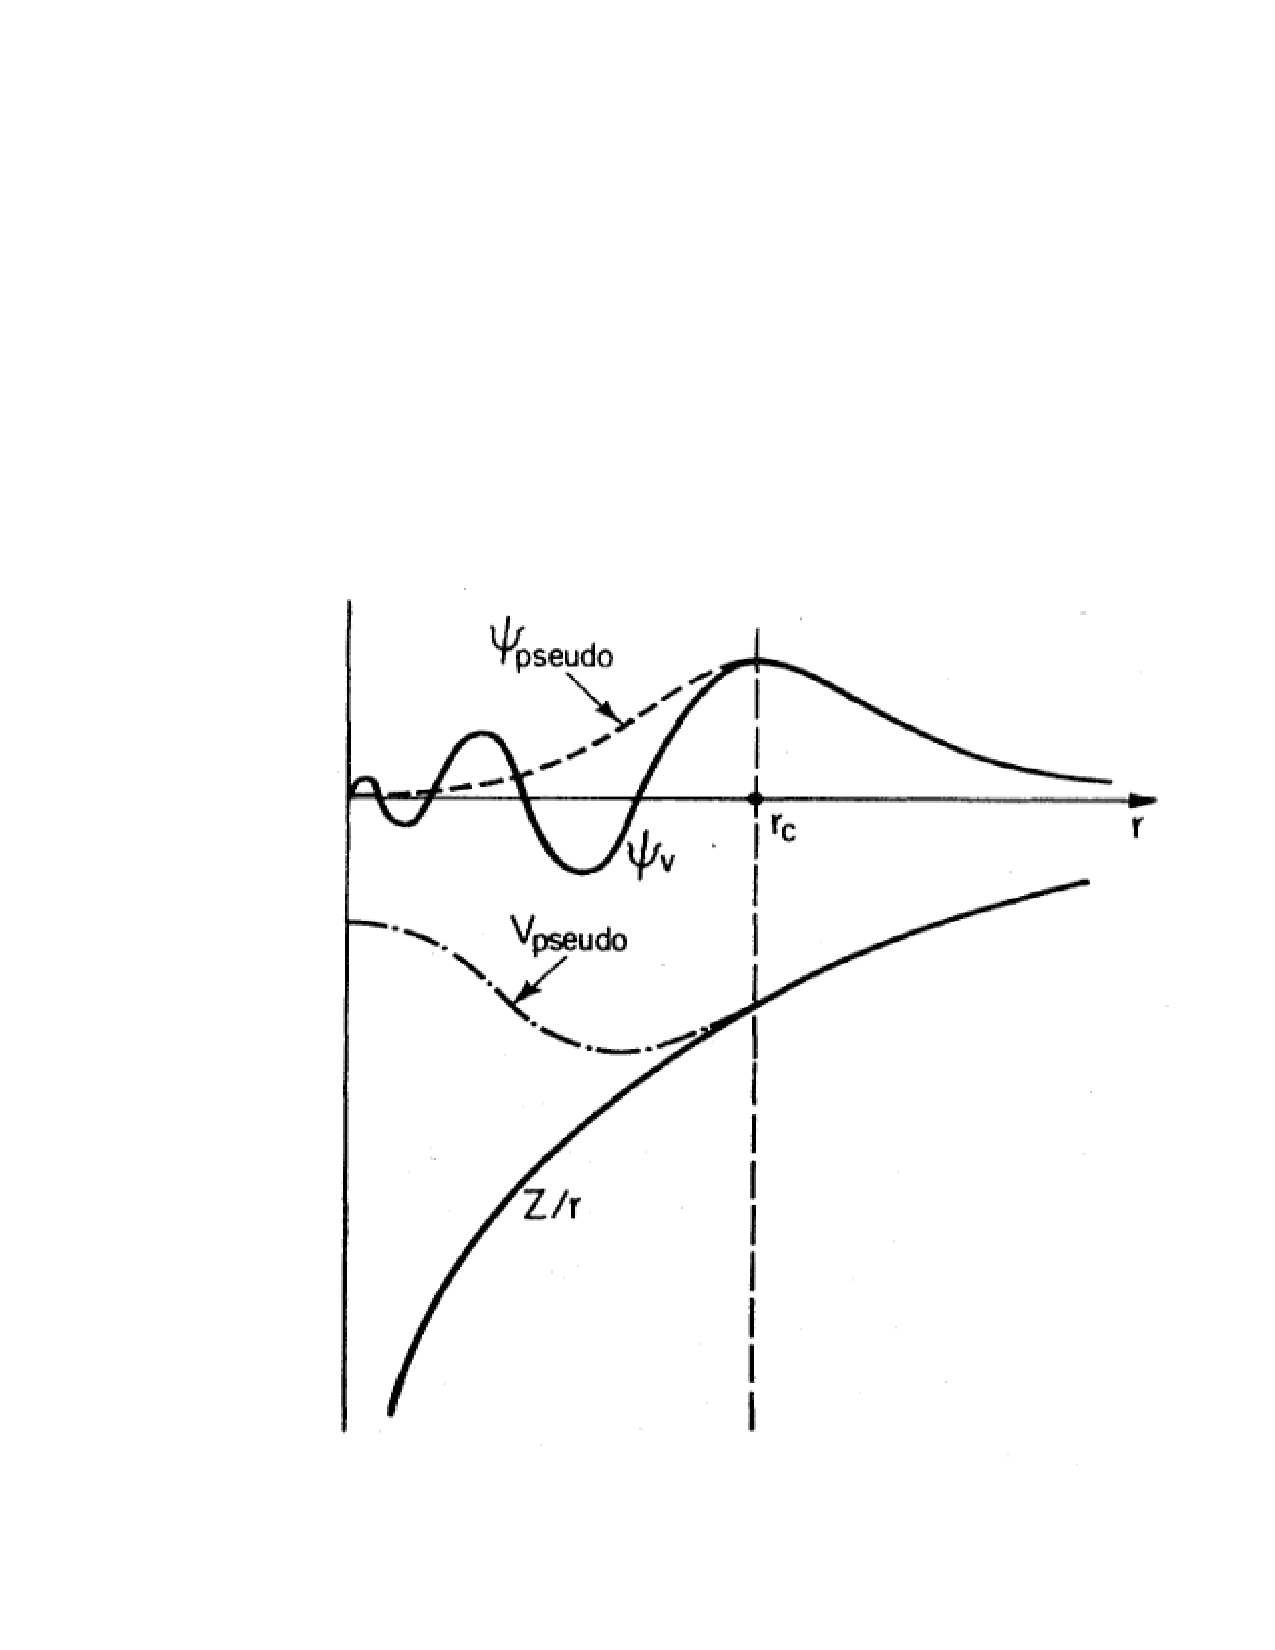
\includegraphics[height=1.35in,width=1.40in,viewport=154 100 562 508,clip]{Figures/Pseudo.pdf}
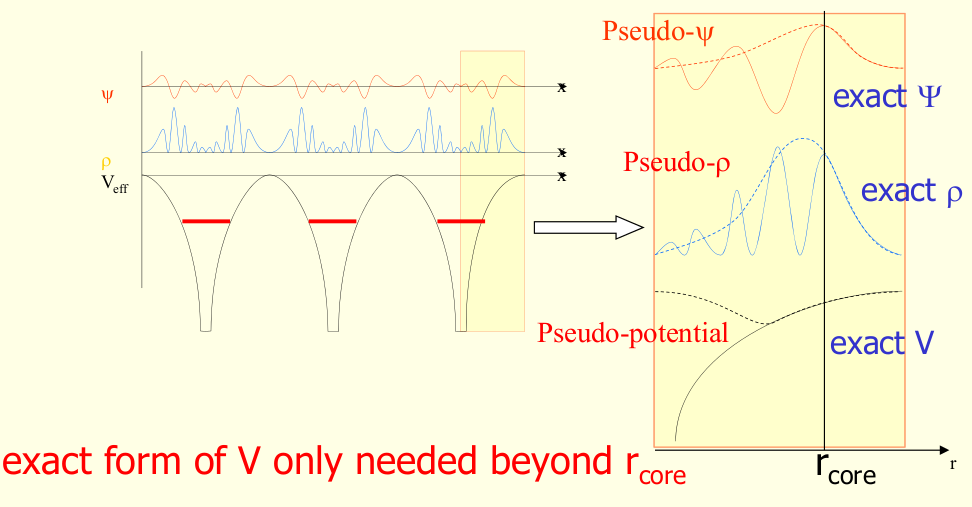
\includegraphics[height=1.35in,width=2.55in,viewport=1 1 980 500,clip]{Figures/Pseudo-2.png}
\caption{\tiny \textrm{The Pseudo wave function and Pseudo potential.}}%(与文献\cite{EPJB33-47_2003}图1对比)
\label{Pseudo_Potential-Wave}
\end{figure}
}

\frame
{
	\frametitle{第一原理赝势}
		由第一原理求解出全电子波函数(径向部分)$P_{n,l}(r)$
			\begin{displaymath}
				\bigg[-\dfrac12\dfrac{\mathrm{d}^2}{\mathrm{d}r^2}+\dfrac{l(l+1)}{2r^2}+V(\rho,r)\bigg]P_{n,l}(r)=\varepsilon_{n,l}P_{n,l}(r)
			\end{displaymath}
			这里$V(\rho,r)$是自洽单电子势
			$$V(\rho,r)=-\frac{Z}r+V_{\mathrm H}(\rho,r)+V_{XC}^{\mathrm{LDA}}(\rho(r))$$
			$V_{\mathrm H}(\rho,r)$是\textrm{Hartree}势,$V_{XC}^{\mathrm{LDA}}(\rho(r))$是交换-相关势

			由此构造赝波函数$P_l^{\mathrm{PP}}(r)$,满足
			$$P_l^{\mathrm{PP}}(r)=P_l^{\mathrm{AE}}(r),\quad r>r_{l}^c$$
			进而构造赝势$V_{\mathrm{src},l}^{\mathrm{PP}}(r)$
			$$V_{\mathrm{src},l}^{\mathrm{PP}}(r)=\varepsilon_l-\dfrac{l(l+2)}{2r^2}+\dfrac{1}{2P_l^{\mathrm{PP}}(r)}\dfrac{\mathrm{d}^2}{\mathrm{d}r^2}P_l^{\mathrm{PP}}(r),\quad r<r_{l}^c$$
}

\frame
{
	\frametitle{模守恒\textrm{(Norm-conserving)}条件}
%	构造赝势确定参数的边界(构造条件)
	\begin{enumerate}
		\item 价电子赝波函数的能量本征值与对应全电子波函数能量本征值相等:~$\varepsilon_l^{\mathrm{PP}}=\varepsilon_l^{\mathrm{AE}}$
		\item 价电子赝波函数与真实电子波函数的径向部分在截断半径$r_{c,l}$外相同:~$\psi_l^{\mathrm{PP}}(r)=\psi_l^{\mathrm{AE}}(r),\quad r>r_{l}^c$
		\item 价电子赝波函数与真实电子波函数的对数导数在截断半径$r_{c,l}$处相等:~$D_l^{\mathrm{PP}}(r)=D_l^{\mathrm{AE}}(r),\quad r\geqslant r_{l}^c$\\
		这里$D_l(\varepsilon,r)=r\frac{\psi_l^{\prime}(\varepsilon,r)}{\psi_l(\varepsilon,r)}=r\dfrac{\mathrm{d}}{\mathrm{d}r}\ln\psi_l(\varepsilon,r)$
		\item 价电子赝波函数与真实电子波函数在截断半径$r_{l}^c$内的积分电荷相等(\textcolor{red}{模守恒条件})
			$$Q_l=\int_0^{r_{l}^c}\mathrm{d}rr^2|\psi_l^{\mathrm{PP}}(r)|^2=\int_0^{r_{l}^c}\mathrm{d}rr^2|\psi_l^{\mathrm{AE}}(r)|^2$$
		\item 价电子赝波函数与真实电子波函数的对数导数一阶能量导数$\mathrm{d}D_l(\varepsilon,r)/\mathrm{d}\varepsilon$在截断半径$r_{l}^c$处及以外相等
	\end{enumerate}
}

\frame
{
	\frametitle{模守恒\textrm{(Norm-conserving)}条件}
\begin{figure}[h!]
\centering
\vspace*{-0.10in}
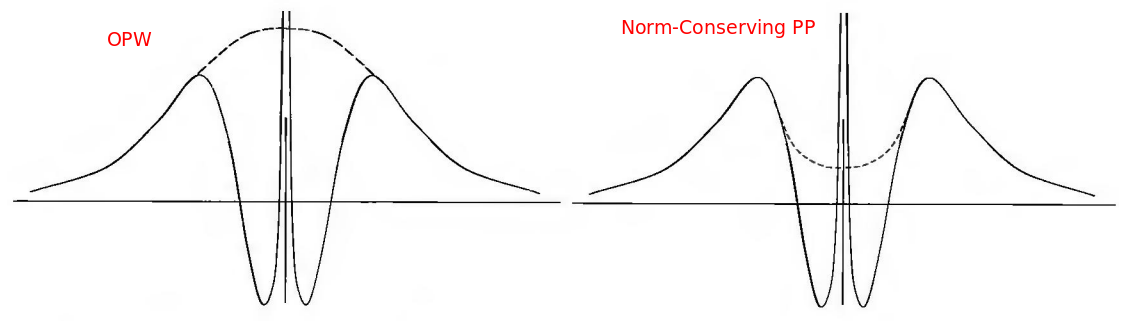
\includegraphics[height=1.30in,width=4.17in,viewport=0 0 1150 350,clip]{Figures/Pseudo-OPW_NCPP.png}
\caption{\tiny \textrm{Schematic example of a valence function that has the character of a $3s$ orbital near the nucleus and two examples of smooth functions (dashed lines) that equal the full wave-function outside the core region. Left: the smooth part of the valence function defined by OPW-like equation; Right: a smooth pseudo-function that satisfies the norm-conservation condition.}}%(与文献\cite{EPJB33-47_2003}图1对比)
\label{Pseudo-OPW_NCPP}
\end{figure}
}

\frame
{
	\frametitle{赝势去屏蔽}
	第一原理赝势建立了赝波函数与对应赝势的一一对应关系,但该赝势包含了电子屏蔽(原子、离子环境)信息,去屏蔽后的赝势对环境依赖更低,“可移植性”更好
	$$V_{\mathrm{ion},l}^{\mathrm{PP}}(r)=V_{\mathrm{src},l}^{\mathrm{PP}}(r)-V_{\mathrm{H},l}^{\mathrm{PP}}(r)-V_{XC,l}^{\mathrm{PP}}(r)$$
	去屏蔽过程中,特别需要注意$V_{XC,l}^{\mathrm{PP}}(r)$的处理
	$$V_{XC,l}^{\mathrm{PP}}(r)=V_{XC}^{\mathrm{PP}}([n_l^{\mathrm{PP}}],r)+\big[V_{XC}^{\mathrm{PP}}([n_l^{\mathrm{PP}}+n^{core}],r)-V_{XC}^{\mathrm{PP}}([n_l^{\mathrm{PP}}],r)\big]$$
}

\frame
{
\frametitle{超软赝势}
\begin{itemize}
\setlength{\itemsep}{5pt}
	\item 赝势构造的模守恒条件
%		\begin{displaymath}
%			\int_0^{r_c}\mathrm{d}\vec r\varphi^{\ast PS}(\vec r)\varphi^{PS}(\vec r)=\int_0^{r_c}\mathrm{d}\vec r\varphi^{\ast}(\vec r)\varphi(\vec r)
%		\end{displaymath}
	很好地解决了赝势可移植性问题,但对$1s$、$2p$、$3d$等轨道,模守恒方案构造的赝势过于“硬”,所需平面波基组依然非常大
	\item 超软\textrm{(Ultra-soft)}赝势,解除模守恒条件,实现对第一、第二周期元素的高效计算
\end{itemize}
\begin{figure}[h!]
\vspace*{-0.10in}
\centering
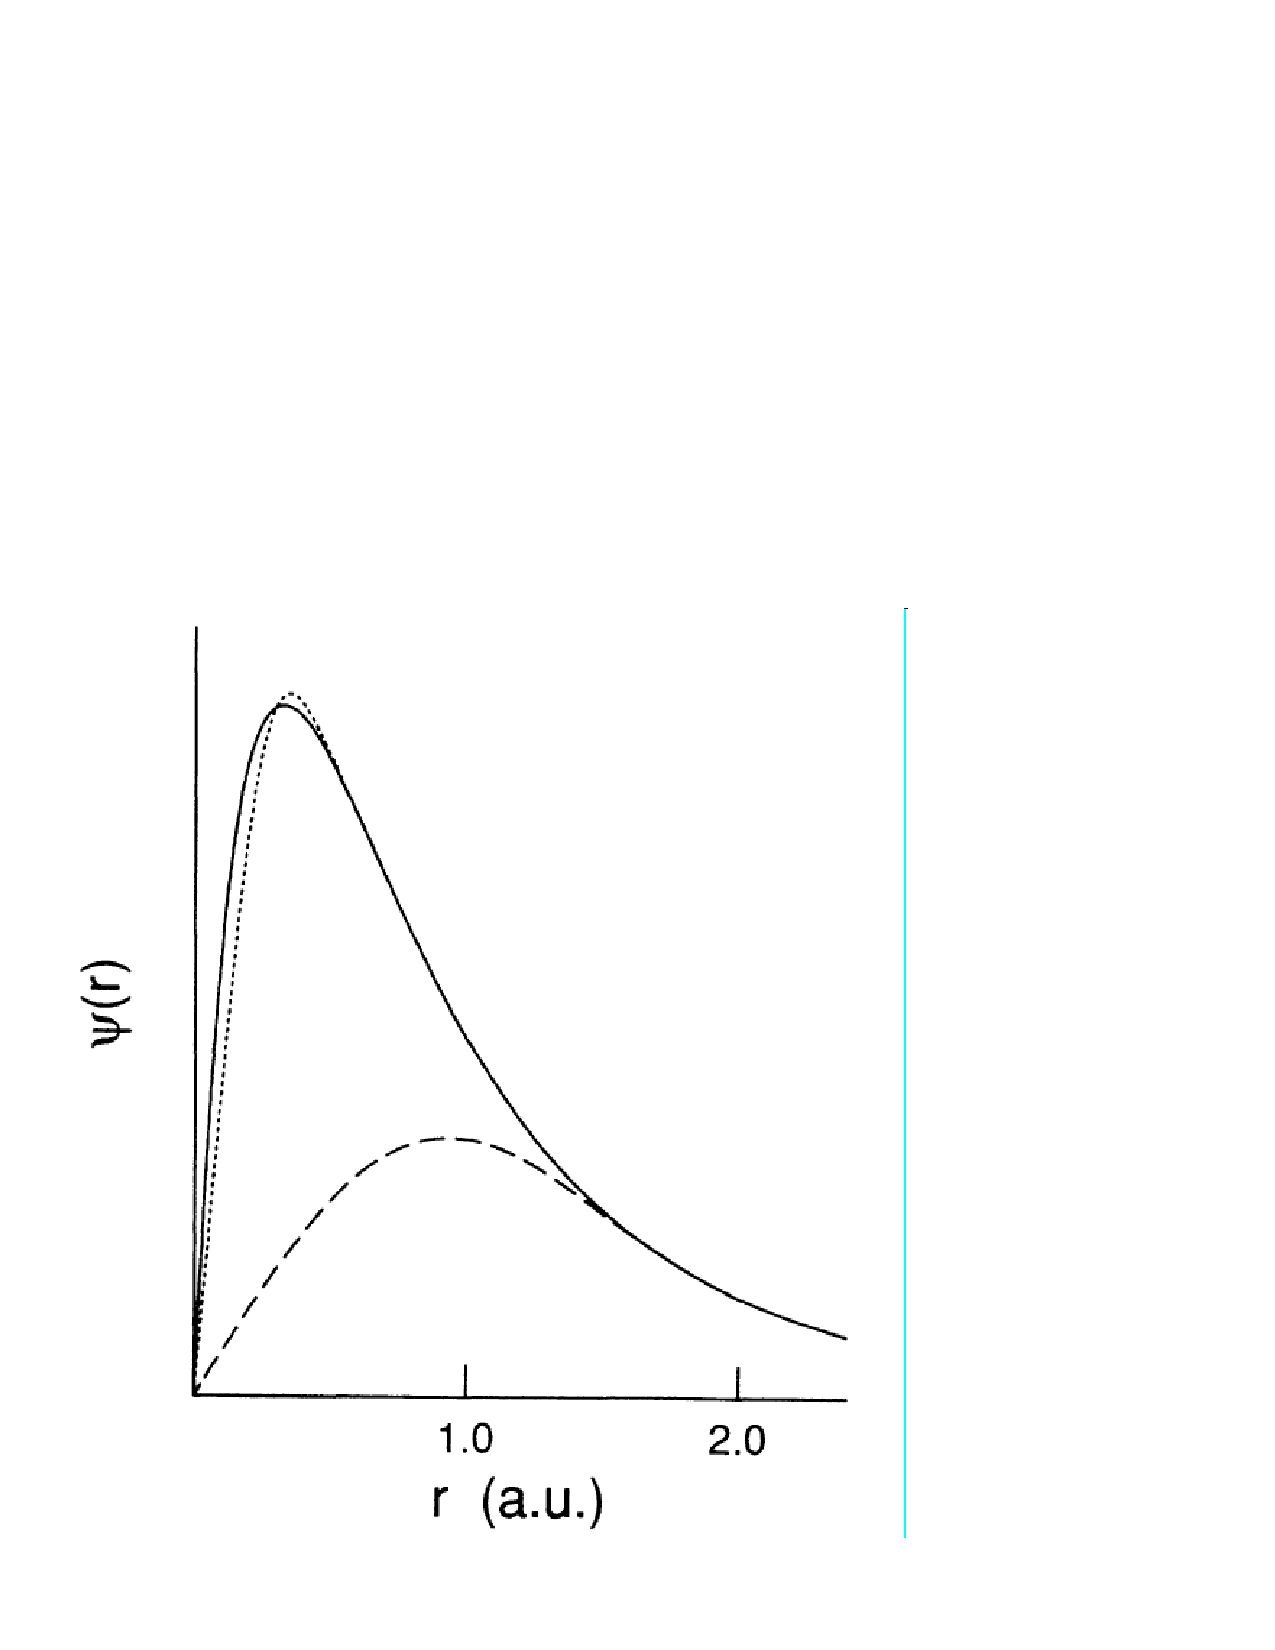
\includegraphics[height=1.35in,width=1.40in,viewport=30 55 415 500,clip]{Figures/Norm-US-wave.pdf}
\caption{\tiny \textrm{Oxygen 2} \textit{p} \textrm{radical wave function (solid), NC-pseudo-wave (dotted) and US-pseudo-wave (dashed).}}%(与文献\cite{EPJB33-47_2003}图1对比)
\label{Norm-US-wave}
\end{figure}
}

\frame
{
\frametitle{补偿电荷与多极矩}
根据电动力学定理:\\\textcolor{blue}{如果球\textrm{S}内的电荷密度分布$\rho(\vec r)$,在球外某点$\vec r$产生的势是由电荷密度的多极矩确定}:
\begin{figure}[h!]
\vspace*{-15pt}
\centering
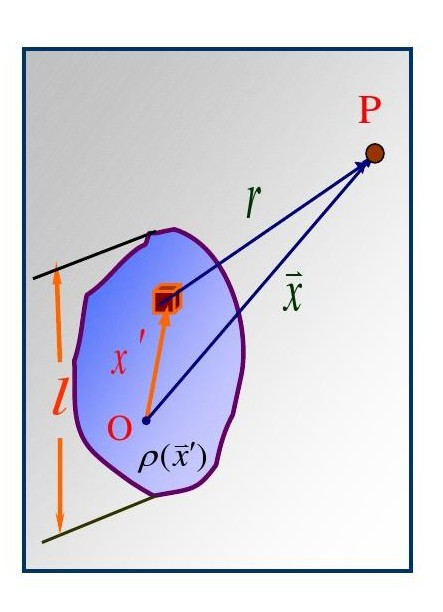
\includegraphics[height=1.25in,width=1.32in,viewport=1 22 507 575,clip]{Figures/potential_multipole.jpg}
%\caption{\tiny \textrm{From Muffin-tin Potential to Full Potential}}%(与文献\cite{EPJB33-47_2003}图1对比)
\label{Potential-multipole}
\end{figure}
\begin{displaymath}
	V(\vec r)=\sum_{l=0}^{\infty}\sum_{m=-l}^{l}\dfrac{4\pi}{2l+1}q_{lm}\dfrac{Y_{lm}(\hat{\vec r})}{r^{l+1}}
\end{displaymath}
其中多极矩$q_{lm}$由下式计算
\begin{displaymath}
	q_{lm}=\int_SY_{lm}^{\ast}(\hat{\vec r})r^l\rho(\vec r)\mathrm{d}^3r
\end{displaymath}
}

\frame
{
\frametitle{超软赝势的构造}
\textrm{Vanderbilt}建议构造赝波函数时放弃模守恒约束条件,只要求价电子赝波函数与真实电子波函数的径向部分在截断半径$r_{l}^c$外相同,由此得到的赝势显然非\textrm{Hermitian},但是通过构造\\\textcolor{blue}{\textrm{Hermitian}重叠算符}
\begin{displaymath}
	\mathbf{S}=\mathbf{1}+\sum_{i,j}Q_{ij}|\beta_j\rangle\langle\beta_i|
\end{displaymath}
以及\textcolor{blue}{\textrm{Hermitian}赝势算符}
\begin{displaymath}
	\tilde V^{\mathrm{NL}}=\sum_{i,j}\mathbf{D}_{i,j}|\beta_j\rangle\langle\beta_i|
\end{displaymath}
这里\textcolor{blue}{
\begin{displaymath}
	\mathbf{D}_{ij}=B_{ij}+\varepsilon_iQ_{ij}
\end{displaymath}}
模守恒约束下的标准本征值方程将变成广义本征值方程
\begin{displaymath}
	(T+V_{\mathrm{loc}}+\tilde V^{\mathrm{NL}}-\varepsilon\mathbf{S})|\phi\rangle=0
\end{displaymath}
}

\frame
{
\frametitle{超软赝势的特点}
\textrm{Vanderbilt}的超软赝势构造方案最大的优点是
\begin{itemize}
	\item \textcolor{purple}{解除模守恒约束}:~有助于增加赝波函数的截断半径,系统提高赝势的柔软程度
	\item \textcolor{purple}{引入多个参考能量$\varepsilon_l$}:~使得模守恒条件下只在特定参考能量$\varepsilon$处成立的对数导数连续条件,扩展到参考能量$\varepsilon_l$区间范围内,这大大提高了赝势的适用范围(可移植性)
\end{itemize}

相应的,超软赝势计算中,电子密度表达形式为
\begin{displaymath}
	n(r)=\sum_nf_n|\phi_n(r)|^2+\sum_{n,ij}f_n\langle\phi_n|\beta_j\rangle\langle\beta_i|\phi_n\rangle Q_{ij}(r)
\end{displaymath}
这里补偿电荷$Q_{ij}(r)$定义为
\begin{displaymath}
	Q_{ij}(r)=\phi_i^{\mathrm{AE}}(r)\phi_j^{\mathrm{AE}}(r)^{\ast}-\phi_i^{\mathrm{US}}(r)\phi_j^{\mathrm{US}}(r)^{\ast}
\end{displaymath}
}

\section{\rm{APW~}与\rm{LAPW~}方法}
\frame
{
\frametitle{\textrm{APW}方法}
\begin{figure}[h!]
\centering
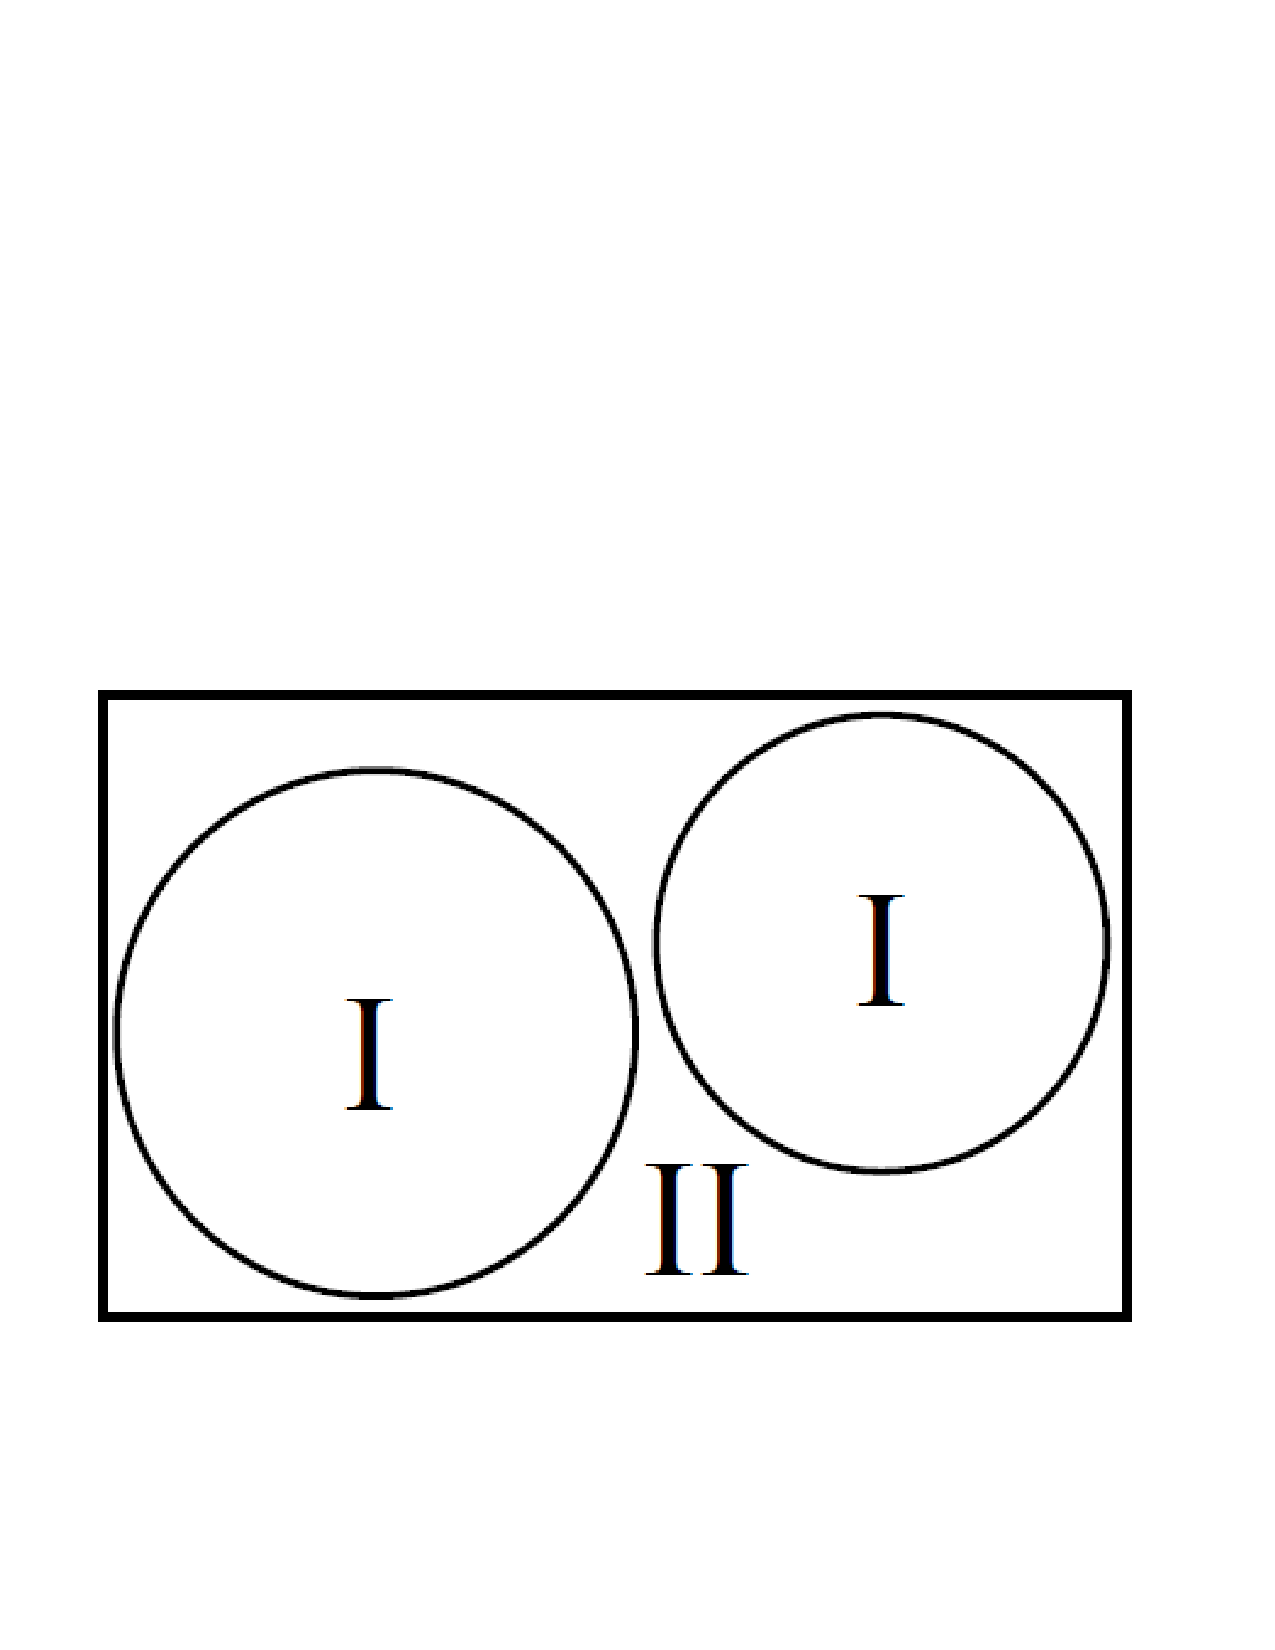
\includegraphics[height=1.10in,width=1.80in,viewport=40 150 545 465,clip]{Figures/Muffin_tin.pdf}
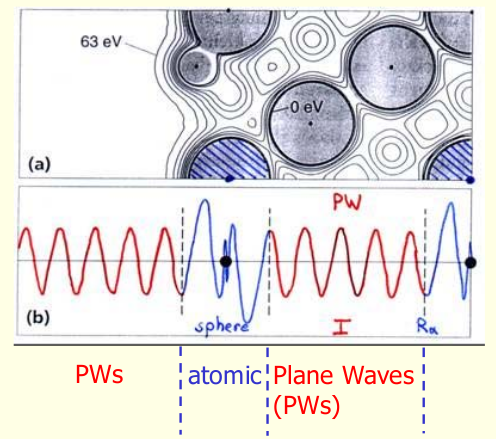
\includegraphics[height=1.10in,width=1.45in,viewport=1 20 485 435,clip]{Figures/APW.png}
\caption{\tiny \textrm{Partitioning of the unit cell into atomic spheres(I) and an interstitial region(II)}}%(与文献\cite{EPJB33-47_2003}图1对比)
\label{Muffin_tin-2}
\end{figure}
\begin{displaymath}
\hskip -28pt\footnotesize \varphi(\vec k_j,\vec r)=\left\{
  \begin{aligned}
    &\Omega^{-1/2}\exp[i\vec k_j\cdot\vec r],&|\vec r-\vec r_s|>R_{\mathrm{MT}}^s\\
    &\sum_{lm}A_{lm}^{\vec k_j}u_l(|\vec r-\vec r_s|,E)Y_{lm}(\widehat{\vec r-\vec r_s}),&|\vec r-\vec r_s|\leqslant R_{\mathrm{MT}}^s
  \end{aligned}
\right.
\end{displaymath}
}

\frame
{
	\frametitle{空间两部分函数在球面上的衔接}
	\textrm{Huygens}原理:~\textcolor{blue}{平面波可以在各个原子球中心用球谐函数展开}:
	\begin{displaymath}
		\mathrm{e}^{\mathrm{i}\vec k\cdot\vec r}=4\pi\sum_{l=0}^{\infty}\sum_{m=-l}^l\mathrm{i}^lj_l(|\vec k|r)Y_{lm}^{\ast}(\hat{\vec k})Y_{lm}(\hat{\vec r})
	\end{displaymath}
	其中$j_l(|\vec k|r)$是$l$-阶球\textrm{Bessel}函数,$\hat{\vec k}$和$\hat{\vec r}$分别是矢量$\vec k$和$\vec r$与直角坐标$z$-轴的夹角$\theta$和$\varphi$

	要求空间中不同区域函数在球面上连续,可调参数$A_{lm}^{\vec k}$可为下式确定
\begin{displaymath}
	A_{lm}^{\vec k}=4\pi\mathrm{e}^{\mathrm{i}\vec k\cdot\vec r_s}\mathrm{i}^lY_{lm}^{\ast}(\hat{\vec k})j_l(|\vec k|R_{MT}^s)/u_l(R_{MT}^s,E)
\end{displaymath}
\textrm{APW}的问题:\textcolor{blue}{球面参数$A_{lm}^{\vec k}$对能量$E$依赖,由此构造的久期方程\footnote{\fontsize{7.2pt}{6.2pt}\selectfont{久期方程\textrm{secular~equation},\textrm{secular}来自拉丁语\textrm{saeculum},本意为一代人、一个时期、一个时代、一个世界等意思。其名词在拉丁语中就作为世纪讲。汉译\textrm{secular}为久期,是取\textrm{long-term}的意思(实为慢,\textrm{slow~in~comparison~to~the~annual~motion}的意思),与期待\textrm{(expectation)}无关。}}非线性的}
}

\frame
{
\frametitle{\textrm{LAPW}方法}
%\small\textrm{APW}方法的困难,久期方程不能化成广义本征值方程的形式(久期方程对能量$E$是非线性的)为了克服这一困难,人们提出线性化方法,
\textrm{O.~K.~Andersen~}提出\textrm{LAPW}方法\upcite{Singh}:将$u_l(r,E)$在某一合适的$E_l$值附近对$E$的一阶微商{$\left.\dfrac{\textrm{d}u_l(r,E)}{\textrm{d}E}\right|_{E_l}\equiv\dot u_l(r,E_l)$}\\代入\textrm{APW}基函数中可得\textrm{LAPW}方法的基函数:
{\fontsize{7.5pt}{3.3pt}\selectfont
$$\hskip -14pt \varphi(\vec k_j,\vec r)=\left\{
  \begin{aligned}
    &\Omega^{-1/2}\exp[i\vec k_j\cdot\vec r],&|\vec r-\vec r_s|>R_{\mathrm{MT}}^s\\
    &\sum_{lm}[A^{\vec k_j}_{lm}u_l(|\vec r-\vec r_s|,E_l)+B^{\vec k_j}_{lm}\dot u_l(|\vec r-\vec r_s|,E_l)]Y_{lm}(\widehat{\vec r-\vec r_s}),&|\vec r-\vec r_s|\leqslant R_{\mathrm{MT}}^s
  \end{aligned}
\right.$$
%$$\Psi_{\vec k}(\vec r)=\int_{\Omega}\tilde G_{\vec k}(\vec r-\vec r\,^\prime;E)V(\vec r\,^\prime)\Psi_{\vec k}(\vec r\,^\prime)\textrm{d}\vec r\,^\prime$$
根据基函数在\textrm{MT}球面上连续到一阶,确定系数$A^{\vec k}_{lm}$,$B^{\vec k}_{lm}$的值。}
\begin{figure}[h!]
	\vskip -3pt
\centering
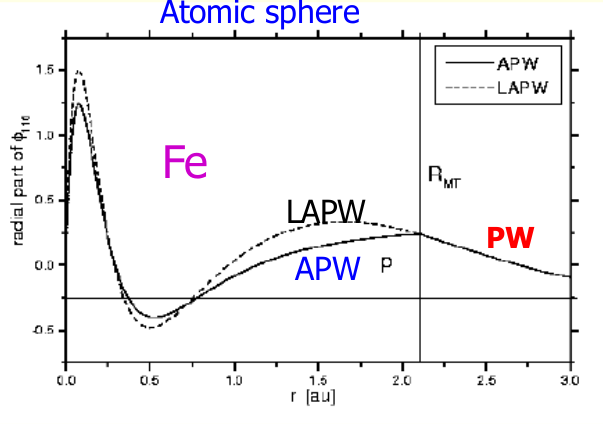
\includegraphics[height=1.10in,width=1.88in,viewport=1 20 585 435,clip]{Figures/WIEN2k-LAPW.png}
\caption{\tiny \textrm{Partitioning of the unit cell into atomic spheres(I) and an interstitial region(II)}}%(与文献\cite{EPJB33-47_2003}图1对比)
\label{Muffin_tin-3}
\end{figure}
}

\section{\rm{MTO~}与\rm{LMTO~}方法}
\frame
{
\frametitle{\textrm{MTO}方法}
\textrm{MTO (Muffin-tin Orbial)}方法是\textrm{Andersen}于\textrm{1971}年提出的局域缀加基函数方案\upcite{Andersen_Book}
%\textrm{MTO}的
\vskip 5pt
\textcolor{blue}{目的:~用最小基组方法解析电子结构}
\begin{itemize}
	\item \textcolor{red}{物理图像}:~和\textrm{APW}方法类似,要求基函数在\textrm{MT}球内、外分区域表示,并且在球面上连续
	\item \textcolor{red}{数学形式}:~基函数是最小优化基组
\end{itemize}
\begin{figure}[h!]
	\vspace{-5pt}
\centering
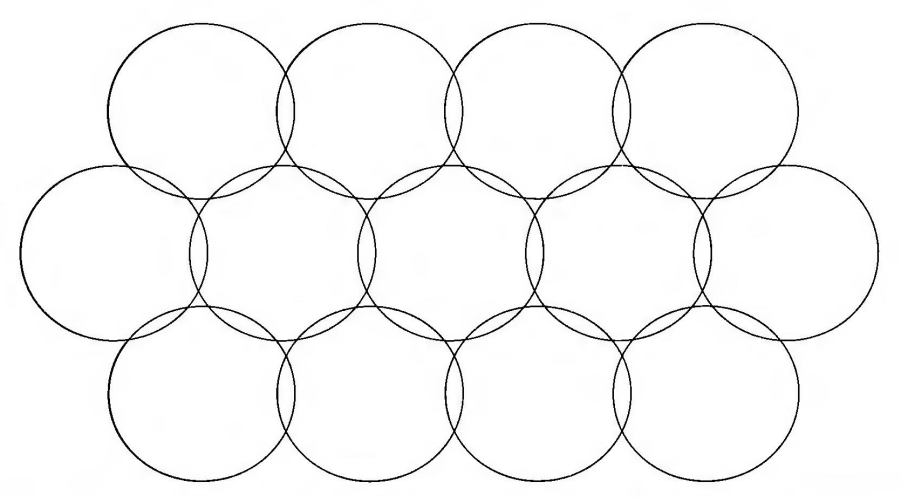
\includegraphics[height=1.20in,width=2.42in,viewport=5 0 1005 495,clip]{Figures/Atomic_sphere-appro.png}
\caption{\fontsize{6.2pt}{4.2pt}\selectfont\textrm{Atomic sphere approximation (ASA) in which the MT spheres are chosen to have the same volume as the Wigner-Seitz cell, which leads to overlapping spheres.}}
\label{Atomic_sphere-appro}
\end{figure}
}

\frame
{
	\frametitle{\textrm{MTO}方法的基函数}
\begin{figure}[h!]
	\vspace{-13pt}
\centering
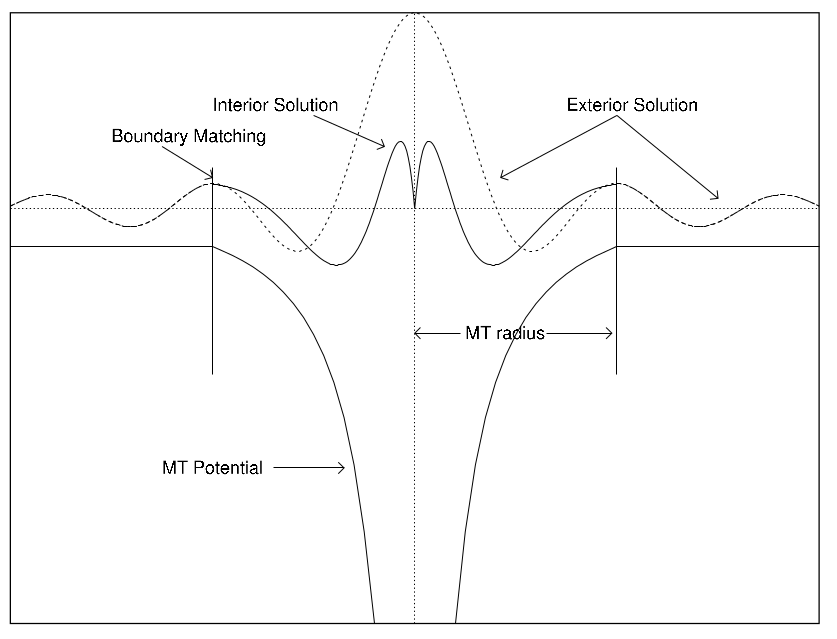
\includegraphics[height=1.25in,width=1.95in,viewport=0 0 845 635,clip]{Figures/MTO-envelope-1.png}
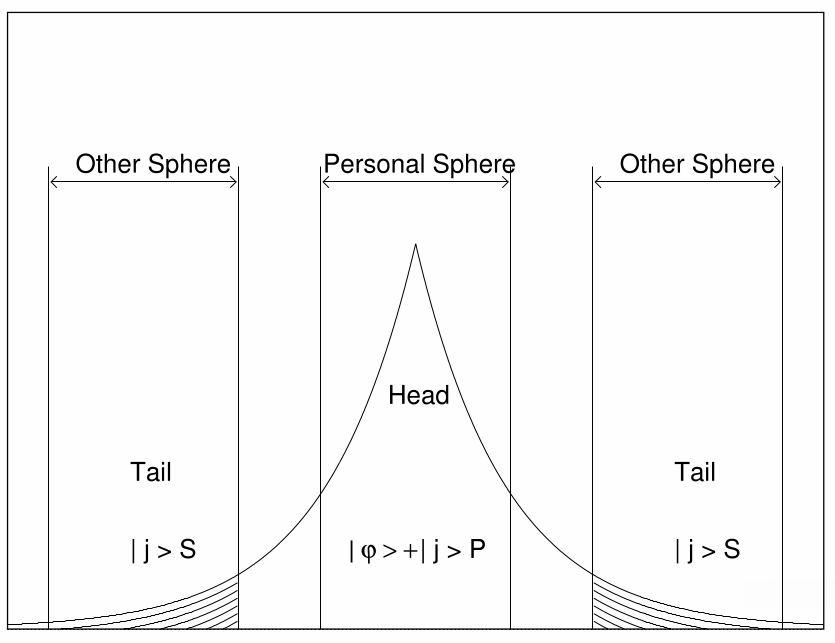
\includegraphics[height=1.25in,width=1.95in,viewport=0 0 885 635,clip]{Figures/MTO-envelope-2.png}
\caption{\tiny \textrm{The radial function of MTO expressed in different region.}}%(与文献\cite{EPJB33-47_2003}图1对比)
\label{MTO-envelope}
\end{figure}
当$q_0=0$时,构成最简单的\textrm{MTO}基函数
		\begin{displaymath}
			\hspace*{-12pt}\chi_L^{\mathrm{MTO}}(\varepsilon,0,\vec r)=\mathrm{i}^lY_L(\hat{\vec r})u_l(\varepsilon,S)\left\{
			\begin{aligned}
				&\dfrac{u_l(\varepsilon,r)}{u_l(\varepsilon,S)}-\dfrac{D_l(\varepsilon)+l+1}{2l+l}\left(\dfrac rS\right)^l&\, r\leqslant S\\
				&+\dfrac{l-D_l(\varepsilon)}{2l+1}\left(\dfrac Sr\right)^{l+1}&\, r>S
			\end{aligned}\right.
		\end{displaymath}
}

\frame
{
	\frametitle{\textrm{MTO}轨道的“尾部抵消”}
\begin{figure}[h!]
	\vspace*{-0.7in}
\centering
\includegraphics[height=2.55in,width=3.15in,viewport=0 0 845 635,clip]{Figures/MTO-Tail_cancellation.png}
\caption{\tiny \textrm{The wavefunction in the spere at the origin is the sum of the ``head function'' in that sphere plus the tails from neighboring spheres. The schematic illustration of the ``tail cancellation'' of the MTO.}}%(与文献\cite{EPJB33-47_2003}图1对比)
\label{MTO-tail-candellation}
\end{figure}
}

\frame
{
	\frametitle{\textrm{LMTO}方法}
	与\textrm{LAPW}方法类似,在给定能量$\varepsilon_v$和衰减常数$q_0$附近,\textrm{LMTO}的基函数球内部分用函数$\psi_l(\varepsilon_v,r)$及其对能量导数$\dot\psi(\varepsilon_v,r)$表示\\
\textcolor{blue}{\textrm{LMTO}与\textrm{MTO}基函数的区别}
	\begin{itemize}
		\item 球内部分的$\psi(\varepsilon,r)$是主要部分:~由$\psi(\varepsilon_v,r)$和$\dot\psi(\varepsilon_v,r)$线性组合
		\item 球内来自其它\textrm{MT}球的函数尾部贡献被$\dot\psi(\varepsilon_v,r)$的线性组合替代
	\end{itemize}
	由此根据物理直觉,可以把\textrm{LMTO}基函数的形式表示成
		\begin{displaymath}
			\hspace*{-12pt}\chi_L^{\mathrm{LMTO}}(\varepsilon,q_0,\vec r)=\mathrm{i}^lY_L(\hat{\vec r})\left\{
			\begin{aligned}
				&u_l(\varepsilon,r)-q_0\cot(\eta_l(\varepsilon))J_l(q_0r)&\, r\leqslant S\\
				&q_0N_l(q_0r)&\, r>S
			\end{aligned}\right.
		\end{displaymath}
		实际应用中,选定函数$J_l$和$N_l$与球\textrm{Bessel}函数$j_l$和\textrm{Neumann}函数$n_l$相似
}

\frame
{
	\frametitle{\textrm{LMTO~.vs.~LAPW}}
\begin{figure}[h!]
\centering
\vspace*{-0.15in}
\includegraphics[height=2.50in,width=3.30in,viewport=0 0 440 350,clip]{Figures/LMTO-vs-LAPW.png}
\caption{\fontsize{5.5pt}{4.2pt}\selectfont{\textrm{Schematic illustration of LMTO vs LAPW.}}}%(与文献\cite{EPJB33-47_2003}图1对比)
\label{LMTO-vs-LAPW}
\end{figure}
}

\section{\rm{PAW}方法}
\frame
{
	\frametitle{\textrm{PAW}方法概要}
\begin{itemize}
	\item 与芯层态正交的全部价电子构成的\textrm{Hilbert}空间%,价电子彼此的正交使得波函数在\textrm{Muffin-tin}球内振荡
	\item 作\textcolor{red}{线性空间变换},全电子波函数$|\Psi\rangle$与赝波函数$|\tilde\Psi\rangle$满足:
		$$|\Psi\rangle=\mathbf{\tau|}\tilde\Psi\rangle$$
%	$$\tau=\mathbf{1}+\sum_{\mathrm R}\hat\tau_{\mathrm R}$$
	\item 在原子核附近的$r_c$范围内,波函数用原子分波函数展开:
	$$|\Psi\rangle=|\tilde\Psi\rangle+\sum_i(|\phi_i\rangle-|\tilde\phi_i\rangle)\langle\tilde p_i|\tilde\Psi\rangle$$
	\item 在$r_c$外$|\tilde\Psi\rangle$与$|\Psi\rangle$变换前后保持不变,因此线性变换$\mathbf{\tau}$可表示为:
	$$\mathbf{\tau}=\mathbf{1}+\sum_i(|\phi_i\rangle-|\tilde\phi_i\rangle)\langle\tilde p_i|$$
\end{itemize}
其中$|\tilde p_i\rangle$是\textrm{MT}球内的投影函数\\
$i$表示原子位置$\vec R$、原子轨道($l,m$)和能级$\epsilon_k$的指标。
}

\frame
{
%	\frametitle{\textrm{PAW}原子数据集}
	\frametitle{\textrm{PAW}方法的基本思想}
\begin{figure}[h!]
\centering
\includegraphics[height=2.3in,width=4.0in,viewport=0 0 1280 745,clip]{Figures/PAW-baseset.png}
\caption{\tiny \textrm{The Augmentation of PAW.}}%(与文献\cite{EPJB33-47_2003}图1对比)
\label{PAW_baseset}
\end{figure}
}

\frame
{
\frametitle{\textrm{PAW}方法的基本思想}
	在赝波函数$|\tilde\Psi\rangle$表象下,算符期望值计算满足$$\langle A \rangle=\langle\Psi|\mathbf{A}|\Psi\rangle=\langle\tilde\Psi|\mathbf{\tau}^{\dag}\mathbf{A}\mathbf{\tau}|\tilde\Psi\rangle=\langle\tilde\Psi|\tilde{\mathrm{A}}|\tilde\Psi\rangle$$
\begin{itemize}
	\item 一般赝算符$\tilde A$表示为
		$$\tilde A=\mathbf{A}+\sum_i|\tilde p_i\rangle(\langle\phi_i|\mathbf{A}|\phi_i\rangle-\langle\tilde\phi_i|\mathbf{A}|\tilde\phi_i\rangle)\langle\tilde p_i|$$
	\item 赝重叠算符$\tilde O$表示为
		$$\tilde O=\mathbf{1}+\sum_i|\tilde p_i\rangle(\langle\phi_i|\phi_i\rangle-\langle\tilde\phi_i|\tilde\phi_i\rangle)\langle\tilde p_i|$$
\end{itemize}
}

\frame
{
\frametitle{\textrm{PAW}方法密度计算}
在\textrm{PAW}框架下,将密度算符$|\vec r\rangle\langle\vec r|$代入,可知密度表达式为
$$n(\vec r)=\tilde n(\vec r)+n^1(\vec r)-\tilde n^1(\vec r)$$
这里
$$\tilde n(\vec r)=\sum_nf_n\langle\tilde\Psi_n|\vec r\rangle\langle\vec r|\tilde\Psi_n\rangle$$ 
$$n^1(\vec r)=\sum_{n,(i,j)}f_n\langle\tilde\Psi_n|\tilde p_i\rangle\langle\phi_i|\vec r\rangle\langle\vec r|\phi_j\rangle\langle\tilde p_j|\tilde\Psi_n\rangle$$
$$\tilde n^1(\vec r)=\sum_{n,(i,j)}f_n\langle\tilde\Psi_n|\tilde p_i\rangle\langle\tilde\phi_i|\vec r\rangle\langle\vec r|\tilde\phi_j\rangle\langle\tilde p_j|\tilde\Psi_n\rangle$$
}

%\frame
%{
%	\frametitle{\textrm{PAW Augmentation}}
%\begin{figure}[h!]
%\centering
%\includegraphics[height=2.3in,width=4.0in,viewport=0 0 1100 745,clip]{Figures/PAW-projector.png}
%\caption{\tiny \textrm{The projector of PAW.}}%(与文献\cite{EPJB33-47_2003}图1对比)
%\label{PAW_projector}
%\end{figure}
%}

\frame
{
\frametitle{电荷密度的重新分解}
\textrm{PAW}方法提出后有很长一段时间没有能够得到广泛应用,直到\textrm{G. Kresse}等将\textrm{Bl\"ochl}的原始方案中电荷密度计算方案重新组合后,明确了\textrm{PAW}方法与\textrm{USPP}方法的内在联系。
\begin{itemize}
	\item 芯层电荷与核电荷构成离子实电荷:$n_{Zc}=n_Z+n_c$
\end{itemize}
\begin{figure}[h!]
\centering
\vspace{-10.5pt}
\includegraphics[height=1.5in,width=3.0in,viewport=0 0 380 190,clip]{Figures/Pseudo-potential_charge.png}
\caption{\tiny \textrm{The difference of the electron-density distributing from P.~Bl\"ochl  and from G.~Kresse.}}%(与文献\cite{EPJB33-47_2003}图1对比)
\label{PAW_Pseudo-Charge}
\end{figure}
}

\frame
{
	\frametitle{固体计算方法总结}
\begin{figure}[h!]
\centering
\vspace*{-0.25in}
%\hspace*{-0.80in}
\includegraphics[height=2.80in,width=4.10in,viewport=0 0 1150 850,clip]{Figures/Pseudo-Full_Potential-2.png}
%\caption{\tiny \textrm{Pseudopotential for metallic sodium, based on the empty core model and screened by the Thomas-Fermi dielectric function.}}%(与文献\cite{EPJB33-47_2003}图1对比)
\label{Pseudo-Full_Poential}
\end{figure}
}

\frame
{
	\frametitle{固体计算软件概览}
\begin{figure}[h!]
\centering
\vspace*{-0.05in}
%\hspace*{-0.80in}
\includegraphics[height=2.30in,width=4.00in,viewport=0 0 920 500,clip]{Figures/DFT-Software.jpg}
%\caption{\tiny \textrm{Pseudopotential for metallic sodium, based on the empty core model and screened by the Thomas-Fermi dielectric function.}}%(与文献\cite{EPJB33-47_2003}图1对比)
\label{Abinitio-Softwares}
\end{figure}
}

%------------------------------------------------------------------------Reference----------------------------------------------------------------------------------------------
		\frame[allowframebreaks]
{
\frametitle{主要参考文献}
\begin{thebibliography}{99}
{\tiny
	\bibitem{Huang-Han}黄昆\:原著、韩汝琦\:改编, {\textit{固体物理学}}\:高等教育出版社, 北京, 1988
	\bibitem{Xie-Lu}谢希德、陆栋\:主编, {\textit{固体能带理论}}\:复旦大学出版社, 上海, 1998
	\bibitem{Elect_Stru}\textrm{Richard. M. Martin. \textit{Electronic Structure: Basic Theory and Practical Methods} (Cambridge University Press, Cambridge, England, 2004)}
        \bibitem{Singh}\textrm{D. J. Singh. \textit{Plane Wave, PseudoPotential and the LAPW method} (Kluwer Academic, Boston,USA, 1994)}					%
	\bibitem{PRB41-7892_1990}\textrm{D. Vanderbilt. \textit{Phys. Rev.} B, \textbf{41} (1990), 7892} 
	\bibitem{Andersen_Book}\textrm{O. K. Andersen. \textit{Computational Methods in Band Theory} (Plenum, New York, USA, 1971)}
	\bibitem{LMTO_Book}\textrm{H. Skriver. \textit{The LMTO method} (Springer, New York, USA, 1984)}
	\bibitem{JPCM6-8245_1994}\textrm{G. Kresse and J. Hafner. J. Phys: \textit{Condens. Matter}, \textbf{6} (1994), 8245}
	\bibitem{PRB50-17953_1994}\textrm{P. E. Bl\"ochl. \textit{Phys. Rev.} B, \textbf{50} (1994), 17953}
	\bibitem{PRB59-1758_1999}\textrm{G. Kresse and D. Joubert \textit{Phys. Rev.} B, \textbf{59} (1999), 1758}
	\bibitem{Nemoshkalenko-Antonov}\textrm{V. V. Nemoshkalenko and V. N. Antonov. \textit{Computational Methods in Solid State Physics} (Gordon and Breach Science Publisher, Amsterdam, The Netherlands, 1998)}
}
\end{thebibliography}
%\nocite*{}
}
\section{计算示例:~\rm{VASP}}
\frame
{
	\frametitle{\textrm{VASP}软件简介}
	\textrm{VASP}软件是维也纳大学\textrm{(Universit\"at Wien)}~\textrm{G. Kresse}等开发的第一原理模拟软件包
	\begin{itemize}
		\item \textrm{VASP}采用\textrm{PAW~(Projector Augmented-Wave)}方法,平衡了赝势方法和全电子计算优点,兼顾了计算的精度和效率
		\item \textrm{VASP}在实空间优化投影函数\textrm{(Projector)},将主要的计算过程变换到实空间完成,大大节省了内存的开销%,保证了计算精度和效率
		\item \textrm{VASP}通过引入多样的优化算法,提高了矩阵对角化和电荷密度搜索的效率
		\item 在\textrm{VASP}的并行计算中,有效均衡了各节点处理\textrm{FFT}变换负载和通信,提升了软件的并行效率
	\end{itemize}
	相比于其他第一原理计算软件,\textrm{VASP}从物理思想与方法、优化算法和并行计算实现等多个方面都有更为出色的性能
}

\frame
{
	\frametitle{\textrm{VASP}的开发团队}
\begin{figure}[h!]
\centering
\vspace*{-0.25in}
\includegraphics[height=2.70in,width=4.05in,viewport=330 130 1280 770,clip]{Figures/VASP_team.png}
\caption{\tiny \textrm{The development team of VASP.}}%(与文献\cite{EPJB33-47_2003}图1对比)
\label{VASP_team}
\end{figure}
}

\frame
{
	\frametitle{\textrm{VASP}的\textrm{Kohn-Sham}方程求解流程}
\begin{figure}[h!]
	\vspace{-0.2in}
\centering
%\includegraphics[height=2.7in,width=4.0in,viewport=0 0 1300 960,clip]{Figures/VASP_procedure-full.png}
%\includegraphics[height=2.1in,width=1.6in,viewport=0 0 480 630,clip]{Figures/VASP_procedure.png}
%\includegraphics[height=2.1in,width=2.3in,viewport=0 0 740 600,clip]{Figures/Ab-initio-Ene.png}
\includegraphics[height=2.75in,width=2.5in,viewport=0 0 480 630,clip]{Figures/VASP_procedure.png}
\caption{\tiny \textrm{The Flow of calculation for the KS-ground states.}}%(与文献\cite{EPJB33-47_2003}图1对比)
\label{PAW_baiseset}
\end{figure} 
}

%\section{\rm{VASP}计算示例}
%\subsection{{\rm Si}的电子结构:~态密度与能带}\label{Sec:Si-band}
%\frame
%{
%	\frametitle{\textrm{Si}的结构:~\textrm{FCC}}
%%{\fontsize{7.2pt}{5.2pt}\selectfont{\textrm{Si}晶胞是金刚石结构,晶胞参数$a_0=5.47\mathrm{\AA}$由结构弛豫确定}}%为了得到\textrm{Si}的电子结构,必须要完成两组连续计算:~即通过静态计算得到迭代收敛的基态电子密度,随后用获得的电子密度,按特定的对称性方向,直接计算(无需自洽迭代)得到能带。
%\textrm{Si}晶胞是金刚石结构,晶胞参数$a_0=5.47\mathrm{\AA}$(由结构弛豫确定)
%\vskip 5pt
%\begin{figure}[h!]
%\centering
%\includegraphics[height=1.6in,viewport=0 0 370 150,clip]{Figures/Si_POSCAR.png}
%%\includegraphics[height=1.8in,width=4.in,viewport=30 210 570 440,clip]{PAW_projector.eps}
%\caption{\fontsize{6.2pt}{5.2pt}\selectfont{\textrm{Si}的原胞:~\textrm{POSCAR}文件.}}%(与文献\cite{EPJB33-47_2003}图1对比)
%\label{Si_POSCAR}
%\end{figure}
%}
%
\frame
{
	\frametitle{\textrm{Si}的初基原胞}
%\textrm{Si}晶胞是金刚石结构,晶胞参数$a_0=5.47\mathrm{\AA}$(由结构弛豫确定)
\vspace*{-13pt}
\begin{figure}[h!]
\centering
\includegraphics[height=1.78in]{Figures/VASP_example-Si_POSCAR-1-Fig.png}
\vskip 1pt
%\includegraphics[height=0.98in]{Figures/VASP_example-Si_POSCAR-1.png}
\includegraphics[height=0.98in,viewport=0 0 370 150,clip]{Figures/Si_POSCAR.png}
%\caption{\tiny \textrm{The structure of TiC.}}%(与文献\cite{EPJB33-47_2003}图1对比)
\label{Fig:VASP-Si_POSCAR}
\end{figure}
}

\frame
{
	\frametitle{\textrm{Si}的初始计算:~输入文件}
\vspace*{-5pt}
\begin{figure}[h!]
\centering
\includegraphics[height=0.62in]{Figures/VASP_example-Si_KPOINTS-G.png}
\vskip 4pt
\includegraphics[height=1.88in]{Figures/VASP_example-Si_INCAR-dyn.png}
%\caption{\tiny \textrm{The structure of TiC.}}%(与文献\cite{EPJB33-47_2003}图1对比)
\label{Fig:VASP-Si_KPOINT-INCAR}
\end{figure}
}

\frame
{
	\frametitle{\textrm{Si}的初始计算:~\textrm{POTCAR}}
\vspace*{-13pt}
\begin{figure}[h!]
\centering
\includegraphics[height=2.88in]{Figures/VASP_example-Si_POTCAR.png}
%\caption{\tiny \textrm{The structure of TiC.}}%(与文献\cite{EPJB33-47_2003}图1对比)
\label{Fig:VASP-Si_POTCAR}
\end{figure}
}

\frame
{
	\frametitle{\textrm{VASP}计算示范:~\textrm{Si}}
\vspace*{-10pt}
\begin{figure}[h!]
\centering
\includegraphics[width=3.0in]{Figures/VASP_example-Si_OUTCAR-1.png}
%\caption{\tiny \textrm{The structure of TiC.}}%(与文献\cite{EPJB33-47_2003}图1对比)
\label{Fig:VASP-Si_OUTCAR-part1}
\end{figure}
}

\frame
{
	\frametitle{\textrm{VASP}计算示范:~\textrm{Si}}
\vspace*{-10pt}
\begin{figure}[h!]
\centering
\includegraphics[width=3.5in]{Figures/VASP_example-Si_OUTCAR-2.png}
%\caption{\tiny \textrm{The structure of TiC.}}%(与文献\cite{EPJB33-47_2003}图1对比)
\label{Fig:VASP-Si_OUTCAR-part2}
\end{figure}
}

\frame
{
	\frametitle{\textrm{Si}的静态计算}
%静态计算是获得电子基态信息的重要步骤,在
静态计算:~确定基态电荷密度
\vskip 2.5pt
{\fontsize{8.5pt}{5.2pt}\selectfont{\textcolor{blue}{材料电子学性质计算的起点}}}
\vskip 3pt
{\fontsize{8.5pt}{5.2pt}\selectfont{静态计算完毕,可以从文件\textrm{OSZICAR}得到体系的基态能量,电荷密度则保存到文件\textrm{CHGCAR}中}}
%\vspace*{-10pt}
\begin{figure}[h!]
\centering
\includegraphics[width=2.5in]{Figures/VASP_cdSi_1.png}
%\caption{\tiny \textrm{The structure of TiC.}}%(与文献\cite{EPJB33-47_2003}图1对比)
\label{Fig:VASP-Si_DOS}
\end{figure}
}

%\subsection{Si的能带结构计算}
\frame
{
	\frametitle{能带计算与$\vec k$点选择}
%一般地,波矢$\vec k $的取值是三维空间(第一\textrm{Brillouin}区)中的矢量。在
	%表\ref{Tabble-kpath}给出的是\textrm{FCC}结构的第一\textrm{Brillouin}区的高对称性$\vec k$点列表。
\begin{minipage}{1.0\textwidth}
\begin{table}[!h]
\tabcolsep 0pt \vspace*{-12pt}
\fontsize{7.2pt}{5.2pt}\selectfont{
%\begin{center}
\centering
\caption{\fontsize{6.2pt}{5.2pt}\selectfont{\textrm{FCC}的第一\textrm{Brillouin}区中高对称性点的列表}}\label{Table-kpath}
\def\temptablewidth{0.95\textwidth}
\renewcommand\arraystretch{0.8} %表格宽度控制(普通表格宽度的两倍)
\rule{\temptablewidth}{1pt}
\begin{tabular*} {\temptablewidth}{@{\extracolsep{\fill}}c@{\extracolsep{\fill}}c@{\extracolsep{\fill}}c}
%-------------------------------------------------------------------------------------------------------------------------
	&\textrm{Reciprocal coordinates} &\textrm{Cartesian coordinates}\\
	\textrm{Points}	&\textrm{(unit of $b_1,b_2,b_3$)} &\textrm{unit of $2\pi/a$} \\\hline
	$\Gamma$ &0~~0~~0 &0~~0~~0 \\
	X &1/2~~0~~1/2 &0~~1~~0 \\
	W &3/4~~1/2~~1/4 &0~~1/2~~1 \\
	L &1/2~~1/2~~1/2 &1/2~~1/2~~1/2 \\
	$\Delta$ &1/4~~0~~1/4 &0~~1/2~~0 \\
	$\Lambda$ &1/ 4~~1/4~~1/4 &1/4~~1/4~~1/4 \\
\end{tabular*}
\rule{\temptablewidth}{1pt}
}
%\end{center}
\end{table}
\end{minipage}
\begin{figure}[h!]
	\vskip -8pt
\centering 
\includegraphics[height=1.7in,viewport=0 0 680 680,clip]{Figures/VASP_train-FCC-BZ.png}
%\includegraphics[height=1.8in,width=4.in,viewport=30 210 570 440,clip]{PAW_projector.eps}
\caption{\fontsize{6.2pt}{5.2pt}\selectfont{\textrm{Brillouin}区为\textrm{FCC}时的空间结构和$\vec k$-点路径关系.}}%(与文献\cite{EPJB33-47_2003}图1对比)
\label{VASP_train-FCC-BZ}
\end{figure}
	{\fontsize{7.5pt}{5.2pt}\selectfont{能带表示中的波矢$\vec k$选择:~沿不可约第一\textrm{Brillouin}区的高对称性点连线}}
%因此,为了绘制平滑的能带曲线,需要在\textrm{KPOINTS}文件中指定足够多的$\vec k$点,能带计算时,只需针对这些指定的$\vec k$点计算各轨道的能量本征值。%如图\ref{Si_KPOINTS}所示:
}

\frame
{
	\frametitle{\textrm{Si}能带计算}

%为了完成能带计算,主要是\textrm{CHGCAR}文件,其余文件改动极少。
%\subsubsection{\rm{INCAR}}%如图\ref{Si_Band-INCAR}所示。这里
%\subsubsection{\rm{KPOINTS}}
{\fontsize{7.5pt}{5.2pt}\selectfont{由\textrm{Brillouin}区$\vec k$点连线,确定\textrm{KPOINTS}文件的$\vec k$点分布:}}\\%如图所示\ref{VASP_train-FCC-BZ}。
{\fontsize{6.2pt}{5.2pt}\selectfont{沿$\vec k$点路线$\mathrm{W}-\mathrm{L}-\Gamma-\mathrm{X}-\mathrm{W}$共计80个$\vec k$点(20点/连线$\times$4组连线)}%的\textrm{KPOINTS}文件%,对应
\begin{figure}[h!]
	\vskip -5pt
\centering 
\includegraphics[width=3.6in,viewport=0 0 540 210,clip]{Figures/Si_KPOINTS.png}
%\includegraphics[height=1.8in,width=4.in,viewport=30 210 570 440,clip]{PAW_projector.eps}
\caption{\fontsize{6.2pt}{5.2pt}\selectfont{\textrm{Si}的能带计算时\textrm{KPOINTS}的设置.}}%(与文献\cite{EPJB33-47_2003}图1对比)
\label{Si_KPOINTS}
\end{figure}
%图\ref{Si_KPOINTS}给出的是\textrm{VASP}计算
}
\begin{figure}[h!] 
	\vskip -5pt
\centering
\includegraphics[height=0.5in,viewport=0 0 330 80,clip]{Figures/Si_Band-INCAR.png}
%\includegraphics[height=1.8in,width=4.in,viewport=30 210 570 440,clip]{PAW_projector.eps}
\caption{\fontsize{6.2pt}{5.2pt}\selectfont{\textrm{Si}的能带计算中的\textrm{INCAR}设置.}}%(与文献\cite{EPJB33-47_2003}图1对比)
\label{Si_Band-INCAR}
\end{figure}
{\fontsize{7.5pt}{5.2pt}\selectfont{静态计算完毕,根据能带计算需要,修改\textrm{INCAR}文件参数:~设置\textcolor{cyan}{\textit{ICHARG}}=11,电荷密度来自静态计算\textrm{CHGCAR},在计算中保持不变}}
}

\frame
{
	\frametitle{\textrm{Si}能带}
%图\ref{Si_Band-DOS}给出绘制的能带图,可见按照当前的$\vec k$点路径选择,。
\begin{figure}[h!]
	\vskip -8pt
\centering
\includegraphics[width=3.5in,viewport=0 10 920 610,clip]{Figures/Si_Band-DOS.png}
%\includegraphics[height=1.8in,width=4.in,viewport=30 210 570 440,clip]{PAW_projector.eps}
\caption{\fontsize{6.2pt}{5.2pt}\selectfont{\textrm{Si}的能带和相应的态密度图,从能带图看出\textrm{Si}是间接带隙半导体.}}%(与文献\cite{EPJB33-47_2003}图1对比)
\label{Si_Band-DOS}
\end{figure}
{\fontsize{6.2pt}{5.2pt}\selectfont{\textrm{Si}是%间接带隙
半导体,带隙$E_g=0.61\textrm{eV}$%是$\Gamma$点和$X$点之间的带隙值,同时也是图中所有$\vec k$点之间最小的能量差。
~(该值仅为实验测得带隙的$1/2$,因\textrm{DFT}先天不足,低估带隙)}}
%不过除了对带隙的低估,\textrm{DFT}计算的色散关系(能量在倒空间分布关系)是完全正确的,比如\textrm{Fermi}面附近有四个价带,四个导带,能量$\varepsilon_{\vec k}^n$随$\vec k$空间的变化逐渐改变,因此\textrm{DFT}理论的计算定性是完全正确的。实际上,其他物理量(比如波函数和电子密度),也和能量本征值有类似的倒空间分布关系。表明这样的$\vec k$点采样是合理的,能够表现物理量在不可约\textrm{Brillouin}区的定量变化。
}

%\frame
%{
%	\frametitle{\textrm{Si}的能带}
%%\vspace*{5pt}
%\begin{figure}[h!]
%\centering
%\includegraphics[width=4.0in]{Figures/VASP_cdSi_2.png}
%%\caption{\tiny \textrm{The structure of TiC.}}%(与文献\cite{EPJB33-47_2003}图1对比)
%\label{Fig:VASP-Si_Band}
%\end{figure}
%}
%
\frame
{
	\frametitle{\textrm{Si}的能带可视化:~\textrm{p4vasp}}
%\vspace*{5pt}
\begin{figure}[h!]
\centering
\includegraphics[width=4.0in]{Figures/VASP_cdSi_3.png}
%\caption{\tiny \textrm{The structure of TiC.}}%(与文献\cite{EPJB33-47_2003}图1对比)
\label{Fig:VASP-Si_p4vasp}
\end{figure}
}

%\subsubsection{\rm{能带中的本征值}}
\frame
{
	\frametitle{\textrm{Si}能带与本征值}
%因为能带计算是非自洽迭代计算,计算出来能量本征值$\varepsilon_{\vec k}^n$写入\textrm{EIGENVAL}文件中,用于绘制能带图。如图\ref{Si_Band-EIGENVAL}所示
	{\fontsize{7.2pt}{5.2pt}\selectfont{由\textrm{OUTCAR}可知\textrm{Fermi}能级为5.6980\textrm{eV}}}%)设为0~\textrm{eV},可以得到$\vec k$点和能量本征值关系的数据文件\textrm{Si-band.dat},内容如图\ref{Si_Band-data}所示
\begin{figure}[h!]
	\vskip -3pt
\centering
\includegraphics[width=4.0in,viewport=0 0 640 375,clip]{Figures/Si_Band-EIGENVAL.png}
%\includegraphics[height=1.8in,width=4.in,viewport=30 210 570 440,clip]{PAW_projector.eps}
\caption{\fontsize{6.2pt}{5.2pt}\selectfont{\textrm{VASP}计算\textrm{Si}的能量本征值文件\textrm{EIGENVAL}(部分).}}%(与文献\cite{EPJB33-47_2003}图1对比)
\label{Si_Band-EIGENVAL}
\end{figure}
%文件\textrm{EIGENVAL}中第一行是倒晶格中的$\vec k$点位置,随后8行是对应的8个能带的能量本征值:~其中前4个(\textrm{No.}~1-4)能级表示价带,是0\textrm{K}下的占据态。从\textrm{EIGENVAL}文件中提取出各$\vec k$点的能量本征值$\varepsilon_{\vec k}^n$,并将\textrm{Fermi}能级设置为0~(可以用本讲义提供的脚本\textcolor{blue}{\textrm{vasp\_to\_image.py}}实现)。运行该脚本,将\textrm{Fermi}能级(

%\begin{figure}[h!]
%\centering
%\includegraphics[height=1.2in,viewport=0 0 540 140,clip]{Si_Band-data.png}
%%\includegraphics[height=1.8in,width=4.in,viewport=30 210 570 440,clip]{PAW_projector.eps}
%\caption{\small \textrm{用于绘制\textrm{Si}能带结构的数据.}}%(与文献\cite{EPJB33-47_2003}图1对比)
%\label{Si_Band-data}
%\end{figure}
}

\section{材料模拟基础:~建模——以\rm{Materials~Studio}为例}
\frame
{
	\frametitle{\textrm{MS}的架构}
\begin{figure}[h!]
\centering
\vspace*{-0.10in}
\includegraphics[height=2.20in,width=4.15in,viewport=0 0 1275 667,clip]{Figures/MS-main_Struct.png}
\caption{\tiny \textrm{The main structure of Materials studio.}}%(与文献\cite{EPJB33-47_2003}图1对比)
\label{MS-main-structure}
\end{figure}
}

%\subsection{\rm{Materials Studio}的界面框架}
\frame
{
	\frametitle{\textrm{MS}的界面框架}
\begin{figure}[h!]
\centering
\vspace*{-0.31in}
\includegraphics[height=2.45in,width=4.10in,viewport=0 0 1340 800,clip]{Figures/MS-Frame.png}
\includegraphics[height=0.45in,width=4.15in,viewport=0 0 1400 147,clip]{Figures/MS-Frame_calculators.png}
\caption{\tiny \textrm{The frame of Materials studio.}}%(与文献\cite{EPJB33-47_2003}图1对比)
\label{MS-Frame}
\end{figure}
}

%\subsection{\rm{Materials Studio:~Building}}
%\frame
%{
%	\frametitle{\textrm{MS:~Building Modules}}
%\begin{figure}[h!]
%\centering
%%\vspace*{-0.10in}
%\includegraphics[height=1.90in,width=4.10in,viewport=0 0 1259 586,clip]{Figures/MS-Building_tools.png}
%\caption{\tiny \textrm{The Building tools in Materials studio.}}%(与文献\cite{EPJB33-47_2003}图1对比)
%\label{MS-Building-tools}
%\end{figure}
%}

%\subsection{\rm{Materials Studio:~Calculator}}
%\frame
%{
%	\frametitle{\textrm{MS:~Calculator}}
%\begin{figure}[h!]
%\centering
%\vspace*{-0.15in}
%\includegraphics[height=2.75in,width=3.80in,viewport=0 0 969 728,clip]{Figures/MS-Caluculator-compare-2.png}
%\caption{\tiny \textrm{Comparing of Calculators in Materials studio.}}%(与文献\cite{EPJB33-47_2003}图1对比)
%\label{MS-Calculator-compare-2}
%\end{figure}
%}
%
%\frame
%{
%	\frametitle{\textrm{MS:~Calculator}}
%\begin{figure}[h!]
%\centering
%%\vspace*{-0.10in}
%\includegraphics[height=1.50in,width=4.10in,viewport=0 0 1517 602,clip]{Figures/MS-Caluculator-compare-1.png}
%\caption{\tiny \textrm{Calculators in Materials studio:~parameters.}}%(与文献\cite{EPJB33-47_2003}图1对比)
%\label{MS-Calculator-compare-1}
%\end{figure}
%}
%
%\frame
%{
%	\frametitle{\textrm{MS:~XC-functionals}}
%\begin{figure}[h!]
%\centering
%\vspace*{-0.10in}
%\includegraphics[height=2.50in,width=4.10in,viewport=0 0 1261 752,clip]{Figures/MS-xc_functional-compare.png}
%\caption{\tiny \textrm{XC-functionals in Materials studio.}}%(与文献\cite{EPJB33-47_2003}图1对比)
%\label{MS-xc_functional-compare}
%\end{figure}
%}
%
\frame
{
	\frametitle{\textrm{MS}的界面框架:~\textrm{Indigo}}
\begin{figure}[h!]
\centering
\vspace*{-0.28in}
\includegraphics[height=2.85in,width=4.15in,viewport=0 0 1140 800,clip]{Figures/MS-Frame_example.png}
\caption{\tiny \textrm{The frame of Materials studio:~Example Indigo.}}%(与文献\cite{EPJB33-47_2003}图1对比)
\label{MS-Frame_example}
\end{figure}
}

%\subsection{\rm{Materials Studio:~Quick Start}}
\frame
{
	\frametitle{\textrm{MS:~Quick Start-01}}
\begin{figure}[h!]
\centering
\vspace*{-0.25in}
\includegraphics[height=2.70in,width=4.10in,viewport=0 0 1134 740,clip]{Figures/MS-New_Project-01.png}
\caption{\tiny \textrm{Quick Start for Materials studio:~Step-01.}}%(与文献\cite{EPJB33-47_2003}图1对比)
\label{MS-Quick_Start-01}
\end{figure}
}

\frame
{
	\frametitle{\textrm{MS:~Quick Start-02}}
\begin{figure}[h!]
\centering
\vspace*{-0.10in}
\includegraphics[height=2.70in,width=4.00in,viewport=0 0 1045 776,clip]{Figures/MS-New_Project-02.png}
\caption{\tiny \textrm{Quick Start for Materials studio:~Step-02.}}%(与文献\cite{EPJB33-47_2003}图1对比)
\label{MS-Quick_Start-02}
\end{figure}
}

\frame
{
	\frametitle{\textrm{MS:~Quick Start-03}}
\begin{figure}[h!]
\centering
\vspace*{-0.10in}
\includegraphics[height=2.68in,width=4.00in,viewport=0 0 1090 760,clip]{Figures/MS-New_Project-03.png}
\caption{\tiny \textrm{Quick Start for Materials studio:~Step-03.}}%(与文献\cite{EPJB33-47_2003}图1对比)
\label{MS-Quick_Start-03}
\end{figure}
}

%\subsection{\rm{Materials Studio:~Modelling}}
\frame
{
	\frametitle{\textrm{MS:~Quick Start-Modelling-01}}
\begin{figure}[h!]
\centering
\vspace*{-0.10in}
\includegraphics[height=2.60in,width=4.00in,viewport=0 0 1090 710,clip]{Figures/MS-New_Project-04.png}
\caption{\tiny \textrm{Quick Start for Materials studio:~Modelling-01.}}%(与文献\cite{EPJB33-47_2003}图1对比)
\label{MS-Quick_Start-Modelling-01}
\end{figure}
}

\frame
{
	\frametitle{\textrm{MS:~Quick Start-Modelling-02}}
\begin{figure}[h!]
\centering
\vspace*{-0.10in}
\includegraphics[height=2.68in,width=4.00in,viewport=0 0 1090 760,clip]{Figures/MS-New_Project-05.png}
\caption{\tiny \textrm{Quick Start for Materials studio:~Modelling-02.}}%(与文献\cite{EPJB33-47_2003}图1对比)
\label{MS-Quick_Start-Modelling-02}
\end{figure}
}

\frame
{
	\frametitle{\textrm{MS:~Modelling Crystal-01}}
\begin{figure}[h!]
\centering
\vspace*{-0.10in}
\includegraphics[height=2.68in,width=4.00in,viewport=0 0 1090 760,clip]{Figures/MS-New_Project-06.png}
\caption{\tiny \textrm{Modelling crystal by Materials studio.}}%(与文献\cite{EPJB33-47_2003}图1对比)
\label{MS-Modelling-Crystal-01}
\end{figure}
}

\frame
{
	\frametitle{\textrm{MS:~Modelling Crystal-02}}
\begin{figure}[h!]
\centering
\vspace*{-0.15in}
\includegraphics[height=2.75in,width=4.00in,viewport=0 0 1090 814,clip]{Figures/MS-New_Project-07.png}
\caption{\tiny \textrm{Modelling crystal by Materials studio:~Parameters.}}%(与文献\cite{EPJB33-47_2003}图1对比)
\label{MS-Modelling-Crystal-02}
\end{figure}
}

\frame
{
	\frametitle{\textrm{MS:~Modelling Crystal-03}}
\begin{figure}[h!]
\centering
\vspace*{-0.15in}
\includegraphics[height=2.75in,width=3.70in,viewport=0 0 818 616,clip]{Figures/MS-New_Project-08.png}
\caption{\tiny \textrm{Modelling crystal by Materials studio:~Lattice-parameters.}}%(与文献\cite{EPJB33-47_2003}图1对比)
\label{MS-Modelling-Crystal-03}
\end{figure}
}

\frame
{
	\frametitle{\textrm{MS:~Modelling Crystal-04}}
\begin{figure}[h!]
\centering
\vspace*{-0.10in}
\includegraphics[height=2.70in,width=4.00in,viewport=0 0 1090 759,clip]{Figures/MS-New_Project-09.png}
\caption{\tiny \textrm{Modelling crystal by Materials studio:~Elements.}}%(与文献\cite{EPJB33-47_2003}图1对比)
\label{MS-Modelling-Crystal-04}
\end{figure}
}

\frame
{
	\frametitle{\textrm{MS:~Modelling Crystal example:~Si}}
\begin{figure}[h!]
\centering
\vspace*{-0.10in}
\includegraphics[height=2.70in,width=2.30in,viewport=0 0 546 747,clip]{Figures/MS-New_Project-10-Si_example.png}
\caption{\tiny \textrm{Modelling crystal by Materials studio:~Si.}}%(与文献\cite{EPJB33-47_2003}图1对比)
\label{MS-Modelling-Crystal-05}
\end{figure}
}

\frame
{
	\frametitle{\textrm{MS:~Modelling Crystal example:~Si}}
\begin{figure}[h!]
\centering
\vspace*{-0.10in}
\includegraphics[height=2.65in,width=4.00in,viewport=0 0 1090 698,clip]{Figures/MS-New_Project-11-Si_crystal.png}
\caption{\tiny \textrm{Modelling crystal by Materials studio:~Si.}}%(与文献\cite{EPJB33-47_2003}图1对比)
\label{MS-Modelling-Crystal-06}
\end{figure}
}

%\subsection{\rm{Materials Studio:~Calculation}}
\frame
{
	\frametitle{\textrm{MS:~CASTEP Calculation example:~Si}}
\begin{figure}[h!]
\centering
\vspace*{-0.10in}
\includegraphics[height=2.62in,width=4.00in,viewport=0 0 1210 740,clip]{Figures/MS-CASTEP-01-Si.png}
\caption{\tiny \textrm{CASTEP Calculation by Materials studio:~Si.}}%(与文献\cite{EPJB33-47_2003}图1对比)
\label{MS-CASTEP-Calculation-01}
\end{figure}
}

\frame
{
	\frametitle{\textrm{MS:~CASTEP Calculation example:~Si}}
\begin{figure}[h!]
\centering
%\vspace*{-0.10in}
\includegraphics[height=2.05in,width=1.95in,viewport=0 0 756 787,clip]{Figures/MS-CASTEP-02-Si-parameter-1.png}
\includegraphics[height=2.05in,width=1.95in,viewport=0 0 775 798,clip]{Figures/MS-CASTEP-02-Si-parameter-2.png}
\caption{\tiny \textrm{CASTEP Calculation by Materials studio:~Parameter.}}%(与文献\cite{EPJB33-47_2003}图1对比)
\label{MS-CASTEP-Calculation-02}
\end{figure}
}

\frame
{
	\frametitle{\textrm{MS:~CASTEP Calculation example:~Si}}
\begin{figure}[h!]
\centering
\vspace*{-0.10in}
\includegraphics[height=2.15in,width=1.95in,viewport=0 -50 650 700,clip]{Figures/MS-CASTEP-13-Si-Calculat-Electron-step.png}
\includegraphics[height=2.15in,width=1.95in,viewport=0 0 636 774,clip]{Figures/MS-CASTEP-13-Si-Calculat-Electron-detail.png}
\caption{\tiny \textrm{CASTEP Calculation by Materials studio:~Electron-step.}}%(与文献\cite{EPJB33-47_2003}图1对比)
\label{MS-CASTEP-Calculation-electron}
\end{figure}
}

\frame
{
	\frametitle{\textrm{MS:~CASTEP Calculation example:~Si}}
\begin{figure}[h!]
\centering
%\vspace*{-0.10in}
\includegraphics[height=1.15in,width=3.30in,viewport=0 0 1070 452,clip]{Figures/MS-CASTEP-03-Si-input-1.png}
\includegraphics[height=1.15in,width=4.00in,viewport=0 0 1070 355,clip]{Figures/MS-CASTEP-03-Si-input-2.png}
\caption{\tiny \textrm{CASTEP Calculation.}}%(与文献\cite{EPJB33-47_2003}图1对比)
\label{MS-CASTEP-Calculation-03}
\end{figure}
}

\frame
{
	\frametitle{\textrm{MS:~CASTEP Calculation example:~Si}}
\begin{figure}[h!]
\centering
\vspace*{-0.10in}
\includegraphics[height=2.65in,width=2.63in,viewport=0 0 643 698,clip]{Figures/MS-CASTEP-04-Si-sever.png}
\caption{\tiny \textrm{CASTEP Calculation by Materials studio:~Connect to localhost.}}%(与文献\cite{EPJB33-47_2003}图1对比)
\label{MS-CASTEP-Calculation-sever}
\end{figure}
}

\frame
{
	\frametitle{\textrm{MS:~CASTEP Calculation example:~Si}}
\begin{figure}[h!]
\centering
\vspace*{-0.10in}
\includegraphics[height=2.60in,width=4.00in,viewport=0 0 1210 740,clip]{Figures/MS-CASTEP-05-Si-Calculat.png}
\caption{\tiny \textrm{CASTEP Calculation by Materials studio:~Run.}}%(与文献\cite{EPJB33-47_2003}图1对比)
\label{MS-CASTEP-Calculation-Run}
\end{figure}
}

\frame
{
	\frametitle{\textrm{MS:~CASTEP Calculation example:~Si}}
\begin{figure}[h!]
\centering
%\vspace*{-0.10in}
\includegraphics[height=1.50in,width=4.00in,viewport=0 0 1070 469,clip]{Figures/MS-CASTEP-06-Si-Calculat-finish.png}
\caption{\tiny \textrm{CASTEP Calculation by Materials studio:~Complete.}}%(与文献\cite{EPJB33-47_2003}图1对比)
\label{MS-CASTEP-Calculation-Complete}
\end{figure}
}

\frame
{
	\frametitle{\textrm{MS:~CASTEP Calculation example:~Si}}
\begin{figure}[h!]
\centering
\vspace*{-0.10in}
\includegraphics[height=2.66in,width=4.00in,viewport=0 0 1150 801,clip]{Figures/MS-CASTEP-07-Si-Calculat-data.png}
\caption{\tiny \textrm{CASTEP Calculation by Materials studio:~Finish.}}%(与文献\cite{EPJB33-47_2003}图1对比)
\label{MS-CASTEP-Calculation-data}
\end{figure}
}

\frame
{
	\frametitle{\textrm{MS:~CASTEP Calculation example:~Si}}
\begin{figure}[h!]
\centering
\vspace*{-0.10in}
\includegraphics[height=2.60in,width=4.00in,viewport=0 0 1039 790,clip]{Figures/MS-CASTEP-08-Si-Calculat-SCF.png}
\caption{\tiny \textrm{CASTEP Calculation by Materials studio:~SCF.}}%(与文献\cite{EPJB33-47_2003}图1对比)
\label{MS-CASTEP-Calculation-SCF}
\end{figure}
}

\frame
{
	\frametitle{\textrm{MS:~CASTEP Analysis example:~Si}}
\begin{figure}[h!]
\centering
\vspace*{-0.10in}
\includegraphics[height=2.60in,width=4.00in,viewport=0 0 1210 742,clip]{Figures/MS-CASTEP-09-Si-Analysis.png}
\caption{\tiny \textrm{CASTEP Analysis by Materials studio.}}%(与文献\cite{EPJB33-47_2003}图1对比)
\label{MS-CASTEP-Analysis}
\end{figure}
}

\frame
{
	\frametitle{\textrm{MS:~CASTEP Analysis example:~Si}}
\begin{figure}[h!]
\centering
\vspace*{-0.10in}
\includegraphics[height=2.66in,width=2.30in,viewport=0 0 567 813,clip]{Figures/MS-CASTEP-10-Si-Analysis-parameter.png}
\caption{\tiny \textrm{CASTEP Analysis by Materials studio:~Parameter.}}%(与文献\cite{EPJB33-47_2003}图1对比)
\label{MS-CASTEP-Analysis-parameter}
\end{figure}
}

\frame
{
	\frametitle{\textrm{MS:~CASTEP Analysis example:~Si}}
\begin{figure}[h!]
\centering
\vspace*{-0.10in}
\includegraphics[height=2.60in,width=4.00in,viewport=0 0 1210 742,clip]{Figures/MS-CASTEP-11-Si-Analysis-charge.png}
\caption{\tiny \textrm{CASTEP Analysis by Materials studio:~Charge.}}%(与文献\cite{EPJB33-47_2003}图1对比)
\label{MS-CASTEP-Analysis-Charge}
\end{figure}
}

\frame
{
	\frametitle{\textrm{MS:~CASTEP Analysis example:~Si}}
\begin{figure}[h!]
\centering
\vspace*{-0.10in}
\includegraphics[height=2.60in,width=4.00in,viewport=0 0 1210 742,clip]{Figures/MS-CASTEP-11-Si-Analysis-display.png}
\caption{\tiny \textrm{CASTEP Analysis by Materials studio:~Display-style.}}%(与文献\cite{EPJB33-47_2003}图1对比)
\label{MS-CASTEP-Analysis-display}
\end{figure}
}

\frame
{
	\frametitle{\textrm{MS:~CASTEP Analysis example:~Si}}
\begin{figure}[h!]
\centering
%\vspace*{-0.10in}
\includegraphics[height=2.00in,width=1.95in,viewport=0 0 810 820,clip]{Figures/MS-CASTEP-12-Si-Analysis-display-parameter-1.png}
\includegraphics[height=2.00in,width=1.95in,viewport=0 0 802 822,clip]{Figures/MS-CASTEP-12-Si-Analysis-display-parameter-2.png}
\caption{\tiny \textrm{CASTEP Analysis by Materials studio:~Display-parameter.}}%(与文献\cite{EPJB33-47_2003}图1对比)
\label{MS-CASTEP-Analysis-display-parameter}
\end{figure}
}

\appendix
\section{经典数值优化算法概要}
\frame
{
	\frametitle{\textrm{Fixed Point}}
	求解方程
	\begin{displaymath}
		f(\mathbf{x})=\mathbf{x}
	\end{displaymath}
	$\mathbf{x}$是函数$f(\mathbf{x})$的\textcolor{red}{不动点}
	
	对这类问题的求解,可以利用迭代关系
	\begin{displaymath}
		\mathbf{x}_{i+1}=f(\mathbf{x}_i)\qquad (i=1,2,3,\cdots)
	\end{displaymath}
	这称为\textcolor{blue}{不动点迭代法}

	{\fontsize{6.2pt}{4.2pt}\selectfont{例如求解方程
	\begin{displaymath}
%		\begin{aligned}
			\lg(10+x)~=~x%\\
			\Longrightarrow	\textcolor{blue}{x\approx 1.04309063}
%		\end{aligned}
		\end{displaymath}}}
\begin{minipage}[b]{0.35\textwidth}
		{\fontsize{3.2pt}{1.2pt}\selectfont{
	\begin{displaymath}
	\vspace{-0.11in}
		\begin{aligned}
			x_0&=1 %~\Longrightarrow 
			\\\lg(10+1)&=1.041392685\\
x_1 &=1.041392685 %~\Longrightarrow 
\\\lg(10+1.041392685)&=1.0430238558\\
x_2 &=1.043023856 %~\Longrightarrow 
\\\lg(10+1.043023856)&=1.0430880104\\
x_3 &=1.043088010 %~\Longrightarrow 
\\\lg(10+1.043088010)&=1.0443090533\\
x_4 &=1.043090533 %~\Longrightarrow 
\\\lg(10+1.043090533)&=1.04430906326\\
x_4 &=1.0430906326 %~\Longrightarrow 
\\\lg(10+1.0430906326)&=1.04430906365\\
x_5 &=1.0430906365 %~\Longrightarrow 
\\\lg(10+1.0430906365)&=1.04430906366\\
x_6 &=1.0430906366 %~\Longrightarrow 
\\\lg(10+1.0430906366)&=1.04430906366
		\end{aligned}
	\end{displaymath}}}
\end{minipage}
\hfill
\begin{minipage}[b]{0.62\textwidth}
\begin{figure}[h!]
	\vspace{-0.21in}
\centering
\includegraphics[height=1.3in,width=2.0in,viewport=0 0 2500 1600,clip]{Figures/solve_lg10.png}
%\caption{\tiny \textrm{The comparison of parallel scaling for ABINIT vs VASP.}}%(与文献\cite{EPJB33-47_2003}图1对比)
\label{solution-log_10}
\end{figure}
\end{minipage}
}

\frame
{
	\frametitle{非线性方程的\rm{Newton~}法求根}
	\textcolor{blue}{不管哪一种数值算法,其设计原理都是将复杂转化为简单的重复,或者说,通过简单的重复生成复杂}:\\
	\textcolor{red}{在算法设计和算法实现过程中,重复就是力量}\\
迭代算法设计:~\textcolor{purple}{“速度”\textrm{vs}“稳定”}
\begin{figure}[h!]
\centering
\animategraphics[autoplay, loop, height=2.0in]{1}{Figures/OP_Newton_}{0}{17}
\label{Equation_Newon}
\end{figure}
}

\frame
{
	\frametitle{迭代优化基本思想}
	对于给定函数$f$,在极值点,函数的梯度满足
	\begin{displaymath}
		\nabla f=0
	\end{displaymath}
	可将函数极值问题转化成方程求根问题
\begin{figure}[h!]
\centering
\includegraphics[height=1.68in,width=1.95in,viewport=30 0 450 360,clip]{Figures/OP_mini-1.png}
\hskip 0.05in
\includegraphics[height=1.68in,width=1.95in,viewport=150 20 560 390,clip]{Figures/OP_mini-2.png}
\label{OP_mini}
\end{figure}
}

\frame
{
	\frametitle{\textrm{Method of steepest descent}}
	对于函数$f(\mathbf{x}_0)$当前位置$\mathbf{x}_0$的负梯度方向$\mathbf{g}_0$满足
	\begin{displaymath}
		\mathbf{g}_0=-\nabla f(\mathbf{x}_0)
	\end{displaymath}
	用$\mathbf{g}_0$方向作为搜索方向,
	\begin{displaymath}
		\mathbf{x}=\mathbf{x}_0+\lambda\mathbf{g}_0,\qquad \lambda>0
	\end{displaymath}
	因为负的梯度方向为当前位置的最快下降方向,所以被称为“\textcolor{blue}{最陡下降法}”\\
	对函数$f$最小化参数$\lambda$,可确定下一步$\mathbf{x}_1$,可有
	\begin{displaymath}
		\dfrac{\mathrm{d}}{\mathrm{d}\lambda}f(\mathbf{x}_0+\lambda\mathbf{g})_0=\mathbf{g}_0\cdot\nabla f(\mathbf{x}_1)=\mathbf{g}_0\cdot\mathbf{g}_1=0
	\end{displaymath}
	因此\textcolor{red}{最速下降法最近邻两步的梯度彼此相互垂直}\\
	\textcolor{purple}{最陡下降法的收敛:~\\靠近极小值时收敛速度减慢,越接近目标,步长越小,前进越慢}
}

\frame
{
	\frametitle{\textrm{Newton-Raphson Method}}
	\textrm{Newton Method}是一种在实数和复数域上近似解方程的方法。\\
	思想:~\textcolor{blue}{用函数的\textrm{Taylor}级数的前几项来寻找方程$f(x)=0$的根}\\
	由\textrm{Newton}迭代公式有
	\begin{displaymath}
		x_{n+1}=x_n-\dfrac{f(x_n)}{f^{\prime}(x_n)}
	\end{displaymath}
	用\textrm{Taylor}级数在$a$附近展开$f(x)$
	\begin{displaymath}
		f(x)=\sum_{n=0}^{\infty}\dfrac{f^{(n)}(a)}{n!}(x-a)^n
	\end{displaymath}
	如果只取其前两项逼近$f(x)$,可有
	\begin{displaymath}
		f(x)=f(a)+f^{(1)}(a)(x-a)
	\end{displaymath}
	不难看出$x=a-\frac{f(a)}{f^{(1)}(a)}$时,有$f(x)=0$
}

\frame
{
	\frametitle{\textrm{Newton-Raphson Method}}
	对于函数求极值问题(函数的导数为零),就转换成
	\begin{displaymath}
		x_{n+1}=x_{n}-\dfrac{f^{(1)}(x_n)}{f^{(2)}(x_n)}
	\end{displaymath}
	对高维函数,一阶导数是梯度,二阶导数是\textcolor{blue}{\textrm{Hessian}矩阵}\\$\mathbf{H}f(\mathbf{x})=[\frac{\partial^2f}{\partial x_i\partial x_j}]_{n\times n}$,有
	\begin{displaymath}
		x_{n+1}=x_n-\alpha[\mathbf{H}f(x_n)]^{-1}\nabla f(x_n)\quad n\geqslant0
	\end{displaymath}
	这里$\alpha$是可调参数%,$\mathbf{H}$是\textrm{Hessian}矩阵

	\begin{itemize}
		\item 最陡下降法是用一个平面去拟合当前位置的局部曲面
		\item \textrm{Newton}法是用一个二次曲面拟合当前位置的局部曲面
	\end{itemize}
通常情况下,二次曲面的拟合会比平面更好,所以牛顿法选择的路径会更符合真实的最优下降路径(收敛更快)

\textcolor{magenta}{\textrm{Newton}法的缺点:~\textrm{Hessian}矩阵求逆的计算成本和复杂度较高}
}

\frame
{
	\frametitle{\textrm{Quasi-Newton Method}}
	\textrm{Newton}法收敛速度快,但计算过程中需计算\textrm{Hessian}矩阵(而且无法保证正定),因此有了\textrm{Quasi-Newton}方法\\
	思想:~\textcolor{blue}{构造可以近似\textrm{Hessian}矩阵(或逆)的正定对称阵}
		{\fontsize{7.2pt}{4.2pt}\selectfont{
	\begin{displaymath}
		f(\mathbf{x})\approx f(\mathbf{x}_{k+1})+\nabla f(\mathbf{x}_{k+1})(\mathbf{x}-\mathbf{x}_{k+1})+\dfrac12(\mathbf{x}-\mathbf{x}_{k+1})\nabla^2f(\mathbf{x}_{k+1})(\mathbf{x}-\mathbf{x}_{k+1})
	\end{displaymath}
	两边作用梯度算符$\nabla$
	\begin{displaymath}
		\nabla f(\mathbf{x})\approx\nabla f(\mathbf{x}_{k+1})+\mathbf{H}_{k+1}(\mathbf{x}-\mathbf{x}_{k+1})
	\end{displaymath}
	当$\mathbf{x}=\mathbf{x}_k$有
	\begin{displaymath}
		\mathbf{g}_{k+1}-\mathbf{g}_k\approx\mathbf{H}_{k+1}(\mathbf{x}-\mathbf{x}_k)
	\end{displaymath}
令
\begin{displaymath}
	\mathbf{s}_k=\mathbf{x}_{k+1}-\mathbf{x}_k\quad\mathbf{y}_k=\mathbf{g}_{k+1}-\mathbf{g}_k
\end{displaymath}
有
\begin{displaymath}
	\mathbf{y}_k\approx\mathbf{H}_{k+1}\cdot\mathbf{s}_k\quad\mbox{或}\quad\mathbf{s}_k\approx\mathbf{H}_{k+1}^{-1}\mathbf{y}_{k}
\end{displaymath}}}
{\fontsize{9.2pt}{4.2pt}\selectfont{\textcolor{purple}{\textrm{Quasi-Newton}法:~靠近极小值时收敛速快;~初值选择不好,易不收敛}}}
}

\frame
{
	\frametitle{共轭梯度的``轭''}
\begin{figure}[h!]
\centering
\includegraphics[height=2.5in,width=4.0in,viewport=0 0 1050 680,clip]{Figures/Yoke_1.png}
\label{Horse_Yoke}
%\caption{\tiny \textrm{Schematic illustration of minimization of a function in two dimensions. The steps 1,2,3,$\cdots$ denote the steepest descent steps and the point $2^{\ast}$ denote the conjugate gradient path that reaches the exact solution after two steps if the functional is quadratic.}}%(与文献\cite{EPJB33-47_2003}图1对比)
\end{figure}
}

\frame
{
	\frametitle{共轭的含义}
\begin{minipage}{0.63\textwidth}
\begin{figure}[h!]
\vskip -23pt
\centering
\includegraphics[height=1.6in,width=2.2in,viewport=0 0 600 490,clip]{Figures/Bi-Yoke_1.jpg}
\vskip 2pt
\includegraphics[height=1.5in,width=2.2in,viewport=0 0 750 530,clip]{Figures/Conjugate_Pi-bond.png}
\label{Conjugate_1}
%\caption{\tiny \textrm{Schematic illustration of minimization of a function in two dimensions. The steps 1,2,3,$\cdots$ denote the steepest descent steps and the point $2^{\ast}$ denote the conjugate gradient path that reaches the exact solution after two steps if the functional is quadratic.}}%(与文献\cite{EPJB33-47_2003}图1对比)
\end{figure}
\end{minipage}
\begin{minipage}{0.35\textwidth}
\begin{figure}[h!]
\centering
\includegraphics[height=2.2in,width=1.5in,viewport=0 0 250 390,clip]{Figures/Conjugate_complex.jpg}
\label{Conjugate_2}
%\caption{\tiny \textrm{Schematic illustration of minimization of a function in two dimensions. The steps 1,2,3,$\cdots$ denote the steepest descent steps and the point $2^{\ast}$ denote the conjugate gradient path that reaches the exact solution after two steps if the functional is quadratic.}}%(与文献\cite{EPJB33-47_2003}图1对比)
\end{figure}
\end{minipage}
}

\frame
{
	\frametitle{\textrm{Conjugate gradient}}
	假设函数在接近极值附件,近似有\textcolor{magenta}{二次函数}的形式
	\begin{displaymath}
		f(\mathbf{x})=f_0+\frac12\mathbf{x}\cdot\mathbf{H}{\mathbf{x}}+\cdots
	\end{displaymath}
	其中$\mathbf{H}$是\textcolor{blue}{\textrm{Hessian}矩阵}%,定义为
%	\begin{displaymath}
%		H_{ij}=\dfrac{\partial^2f(\mathbf{x})}{\partial x_i\partial x_j}
%	\end{displaymath}
	当$f$的偏导连续,则$\mathbf{H}$是对称矩阵,并且一般要求$\mathbf{H}$是正定的。相应的梯度表示为
	\begin{displaymath}
		\mathbf{g}=\nabla f(\mathbf{x})=-\dfrac{\partial f}{\partial\mathbf{x}}=-\mathbf{H}\cdot\mathbf{x}
	\end{displaymath}
	\vskip 20pt
	设从点$\mathbf{x}_i$出发沿方向$\mathbf{h}_i$(\textcolor{blue}{不再限于梯度$\mathbf{g}_i$方向}),前进到点$\mathbf{x}_{i+1}$,根据最小化要求
	\begin{displaymath}
		\mathbf{h}_i\cdot\nabla f(\mathbf{x}_{i+1})=0
	\end{displaymath}
	为确定$\mathbf{x_{i+1}}$点的继续前进方向$\mathbf{h}_{i+1}$,设$\mathbf{x}_{i+1}$可由$\mathbf{x}_i+\lambda\mathbf{h}_{i+1}$得到,因此$\mathbf{x}_{i+1}$的梯度
	\begin{displaymath}
		\mathbf{g}_{i+1}=\nabla f(\mathbf{x}_{i+1})=-\mathbf{H}\mathbf{x}_{i+1}=-\mathbf{H}(\mathbf{x}_{i}+\lambda\mathbf{h}_{i+1})
	\end{displaymath}
}

\frame
{
	\frametitle{\textrm{Conjugate gradient}}
	与方向$\mathbf{h}_i$相比,梯度的改变为
	\begin{displaymath}
		\Delta\mathbf{g}=-\lambda\mathbf{H}\mathbf{h}_{i+1}
	\end{displaymath}

	根据最小化要求,梯度的改变与$\mathbf{h}_i$方向正交
	\begin{displaymath}
		\mathbf{h}_i\cdot\mathbf{H}\cdot\mathbf{h}_{i+1}=0
	\end{displaymath}
	共轭梯度法算法:对于给定函数
	\begin{itemize}
		\item 已知初值$\mathbf{x}_0$和梯度$\mathbf{g}_0$,取初始方向$\mathbf{h_0}=\mathbf{g}_0$(\textcolor{blue}{最陡下降})
		\item 根据递推关系确定
			\begin{displaymath}
				\begin{aligned}
					\mathbf{g}_{i_+1}=&\mathbf{g}_{i_+1}-\lambda_i\mathbf{H}\mathbf{h}_{i}\qquad \lambda_i=\dfrac{\mathbf{g}_i\cdot\mathbf{g}_i}{\mathbf{g}_i\cdot\mathbf{H}\mathbf{h}_i}\\	
					\mathbf{h}_{i_+1}=&\mathbf{g}_{i_+1}+\gamma_i\mathbf{h}_{i}\qquad \gamma_i=-\dfrac{\mathbf{g}_{i+1}\cdot\mathbf{H}\mathbf{h}_i}{\mathbf{h}_i\cdot\mathbf{H}\mathbf{h}_i}\\	
					\mathbf{x}_{i_+1}=&\mathbf{x}_{i}+\lambda_i\mathbf{h}_{i}
				\end{aligned}
			\end{displaymath}
	\end{itemize}
	\textcolor{purple}{共轭梯度法的收敛:~步收敛性,稳定性高,不需要任何外来参数}
}

\frame
{
	\frametitle{最陡下降与共轭梯度}
\begin{figure}[h!]
\centering
\includegraphics[height=2.0in,width=3.5in,viewport=0 0 950 590,clip]{Figures/OP_descent_CG.png}
\label{decent_CG}
\caption{\tiny \textrm{Schematic illustration of minimization of a function in two dimensions. The steps 1,2,3,~$\cdots$ denote the steepest descent steps and the point - \!- \!- \!- \!- \!- denote the conjugate gradient path that reaches the exact solution after two steps if the functional is quadratic.}}%(与文献\cite{EPJB33-47_2003}图1对比)
\end{figure}
}

\subsection{矩阵的迭代对角化}
\frame
{
	\frametitle{矩阵的迭代对角化}
	\begin{itemize}
		\item 矩阵的直接对角化计算复杂复 $O(N^3)$
		\item 矩阵的迭代对角化计算复杂度 $O(N_0^2\times N\ln N)\quad N_0\ll N$
	\end{itemize}
	\textcolor{blue}{迭代求本征值的思想是\textrm{Jacobian~}于\textrm{1846~}年提出的}\\
	其基本思想是
	\begin{displaymath}
		(H-\varepsilon^n)|\psi^n\rangle=|R[\psi^n]\rangle
	\end{displaymath}
	这里$n$是迭代步数,$|\psi^n\rangle$和$\varepsilon^n$分别是本征态和本征值,$|R[\psi^n]\rangle$是残差矢量
	\vskip 10pt
	{\fontsize{7.2pt}{1.2pt}\selectfont{
	在电子态计算过程中,选择适当的基函数,可以使\textrm{Schr\"odinger~}方程的矩阵接近对角阵\\因此可有
	\begin{displaymath}
		\begin{aligned}
			|\psi^{n+1}\rangle=&\mathbf{D}^{-1}(\mathbf{H}-\varepsilon)|\psi^n\rangle+|\psi^n\rangle=\delta|\psi^{n+1}\rangle+|\psi^n\rangle\\
			\mathbf{D}\delta\psi^{n+1}=&R[\psi^n]\quad \mbox{或}\quad \delta\psi^{n+1}=\mathbf{D}^{-1}R[\psi^n]\equiv\mathbf{K}R[\psi^n]
		\end{aligned}
	\end{displaymath}
	这里$\mathbf{D}$是非奇异矩阵,与$\mathbf{H}$矩阵有关\\
	$\mathbf{K}=\mathbf{D}^{-1}$,也叫''预处理矩阵'',可根据需要选取多种形式
	\begin{itemize}
		\item 要求$\mathbf{D}$比原始的$\mathbf{H}-\varepsilon$更易求逆阵
		\item 要求$\mathbf{D}$使得修正项$\delta\psi^{n+1}$能够使$\psi^n$尽可能更接近正确的本征矢
	\end{itemize}
}}
}

\frame
{
	\frametitle{矩阵迭代对角化的基本思想}
\begin{figure}[h!]
\centering
\includegraphics[height=2.5in,width=3.5in,viewport=0 0 850 590,clip]{Figures/Coordinate_transformation.png}
\label{decent_CG}
\caption{\tiny \textrm{Schematic illustration of searching for the eigenvalue of a vector.}}%(与文献\cite{EPJB33-47_2003}图1对比)
\end{figure}
}

